\chapter{Regularization and the Interpretation of CCA Weights and Loadings}\label{chap:als}
\minitoc
% chktex-file 44 
% chktex-file 3
This chapter expands on my work previously showcased at the OHBM conference and draws connections to a tutorial paper I co-authored, where I contributed a number of simulations\citep{mihalik2022canonical}.

\section{Introduction}\label{sec:introduction}

This chapter explores the role of regularization in improving the performance and interpretation of Canonical
Correlation Analysis (CCA) using simulated and real data from the Human Connectome Project (HCP) and Alzheimer's Disease Neuroimaging Initiative (ADNI) datasets.

The application of Canonical Correlation Analysis (CCA) methods to practical problems often involves two key aspects: predicting latent variables associated with different views, and understanding the nature of the relationship between these views.
This dichotomy in goals bears resemblance to the distinction between machine learning and probabilistic or statistical approaches to the CCA problem.
Machine learning approaches prioritize (out-of-sample) prediction of latent variables for downstream tasks, while statistical approaches seek to infer the data generation process from latent variables to the observed data.
Notably, the probabilistic approach to CCA focusses on the forward model from latent variables to observed data, while the machine learning approach focusses on the inverse model from observed data to latent variables.
As a result the probabilistic CCA is parameterized by the \textit{loadings}, while the machine learning approach is parameterized by \textit{weights}.
We would ideally like to have the best possible prediction of the latent variables, while also being able to interpret the model and understand the relationship between the views.

In addition, CCA models often exhibit shortcomings when dealing with high-dimensional data.
This challenge is particularly acute in brain-behavior studies.
In these studies, neuroimaging modalities typically have a much higher dimensionality than the available sample size.
In this context, CCA models are prone to overfitting, leading to spurious correlations and poor generalization.
Regularization, having been extensively studied and well-understood in the contexts of Linear Regression and Inverse Problems, introduces a deliberate bias to guide models towards more generalizable solutions.
This principle, when applied to CCA, offers a promising avenue for addressing its challenges, ensuring that the model does not overfit to the noise in the data but captures the true underlying patterns.
Furthermore, regularization can help us improve the interpretability of the results most clearly by encouraging sparsity.

In this chapter, we reexamine the relationship between machine learning and probabilistic CCA approaches using simulated data. 
We demonstrate that these approaches are more aligned than previously thought. 
While sparse regularization of CCA weights can lead to sparse estimates of generative model loadings in some conditions, it doesn't always ensure sparse loadings, especially under anisotropic noise. 
Furthermore, regularization can enhance performance in low SNR scenarios, but using the PLS objective can introduce bias, emphasizing dominant principal components and overshadowing subtler correlations.

With this perspective in mind, we propose a flexible regularized alternating least squares (FRALS) framework for CCA which allows us to incorporate any regularized least squares solver to efficiently implement a wide range of regularization functions, but in particular allows us to efficiently implement the elastic net with controllable L2 and L1 penalties so that we can control the bias towards the largest principal components while still encouraging sparsity in the weights.
This is in contrast to much of the previous work on sparse Brain-Behavior analysis which has used a PLS objective with lasso constraints (SPLS), which inherits a bias towards the largest principal components from PLS.

We apply FRALS with ElasticNet regularization to the Human Connectome Project (HCP) dataset, and show that it outperforms other CCA models in terms of out-of-sample canonical correlation.
We also show that the identified mode of variation is distinct from previous work which identified latent variables with loadings related to cognitive tests and negatively related to cigarette, tobacco or alcohol\citep{smith2015positive}.
FRALS has stronger correlations with the Line Orientation test, which measures visuospatial abilities, and the parietal lobe, which is known to be involved in visuospatial processing.
This further demonstrates the importance of matching the model to the data generation process with the appropriate regularization.

\section{Background}\label{sec:background}

To understand how to interpret the weights of CCA models and therefore how to regularize the CCA problem, we first review probabilistic and generative perspectives on CCA. Then we review previous work on regularized CCA with a focus on ridge (L2), lasso (L1), and elastic net (L1 + L2) regularization.

\subsection{Generative Perspectives on CCA}\label{subsec:generative-perspectives-on-cca}
Understanding the data generation process in Canonical Correlation Analysis (CCA) and Partial Least Squares (PLS) is pivotal for many reasons.
It influences the choice of appropriate models, evaluation metrics, and sheds light on the underlying structure and dependencies between views.
Probabilistic formulations provide a principled framework to understand this process, helping us gauge the assumptions we make and the limitations these impose.

\subsubsection{A probabilistic latent variable perspective on CCA}\label{subsubsec:a-probabilistic-latent-variable-perspective-on-cca}

Consider the graphical model depicted in Figure~\ref{fig:mentalhealthselfsupervised}.
It comprises two distinct views: a neuroimaging modality and a behavioral modality.
Both views are assumed to originate from a common latent variable, representing the severity of a mental health condition.
The neuroimaging modality is generated via a linear model with added noise, while the behavioral modality similarly arises from a linear model with noise.
Consequently, the brain and behavioral modalities exhibit correlation since they both derive from the same latent variable.
In a statistical sense, they are conditionally independent, given the latent variable.

\begin{figure}
    \centering
    \tikz{
        % nodes
        \node[latent, align=center, minimum size=2cm] (Z) {Severity\\z};
        %
        \node[obs, below left=of Z, minimum size=2cm] (x1) {Brain       $x\sps{1}$};%
        \node[obs, below right=of Z, minimum size=2cm] (x2) {Behaviour  $x\sps{2}$};%
        % edges
        \edge{Z} {x1}
        \edge{Z} {x2}}
    \caption[Latent Variable Model of Mental Health]{\textit{\textbf{Latent Variable Model of Mental Health:}} From this perspective the neuroimaging modality and behavioural data are both considered to have been generated with distributions conditioned on the severity of a mental health condition}\label{fig:mentalhealthselfsupervised}
\end{figure}

The distributions of the two views are given by:

\begin{align}
    z& \sim \mathcal{N}(0, I)\\
    x\sps{i} & \sim \mathcal{N}(W\sps{i} z + \mu\sps{i}, \Psi\sps{i})
\end{align}

Where \(z\) represents the latent variable (disease severity), \(x\sps{i}\) represents the $i^{\text{th}}$ view, \(W\sps{i}\) represents the model loadings, \(\mu\sps{i}\) represents the mean, and \(\Psi\sps{i}\) represents the noise covariance matrix for the $i^{\text{th}}$ view. 
Notice that if it were not for the view-specific noise, the two views would be perfectly correlated subject to a linear transformation.

\citep{bach2005probabilistic} showed that the maximum likelihood solution for this model is equivalent to the solution of the CCA problem in the sense that the loadings are the same as the CCA weights multiplied by the sample covariance:

\begin{align}\label{eq:probabilistic-cca}
    \hat{W}\sps{i} = \hat{\Sigma_{ii}} \hat{U}\sps{i} R
\end{align}

Where $R$ is an arbitrary rotation matrix and $\hat{U}\sps{i}$ is the matrix of CCA weights for the $i$th view.
This implies that for invertible covariance matrices, we can access the `true' CCA weights by multiplying the loadings by the inverse of the covariance matrix:

\begin{align}
    \hat{U}\sps{i} = \hat{\Sigma_{ii}}^{-1} \hat{W}\sps{i}
\end{align}

Notice that for Identity covariance matrices, the CCA weights are the same as the loadings.
Otherwise, there is a linear transformation between the two.
For singular covariance matrices, the CCA weights are not uniquely defined.

Moreover, the mean of the posterior distribution of the latent variables is proportional to the mean of the CCA scores\citep{klami2013bayesian}.
Group Factor Analysis (GFA) is a closely related model that assumes diagonal covariance in $\Psi\sps{i}$:

\begin{align}
    z& \sim \mathcal{N}(0, I)\\
    x\sps{i} & \sim \mathcal{N}(W\sps{i} z, \sigma\sps{i}I)
\end{align}

An interesting feature of the GFA model is that as the noise level approaches zero, the marginal distribution of the views is the same as the probabilistic PCA model for each view~\citep{tipping1999probabilistic}.
This suggests that for small noise levels, we should in fact be able to recover much of the mutual information between the views by using PCA on each view separately.
For this reason, we will use and recommend PCA as a baseline in our later experiments.
Because the diagonal covariance assumption makes inference computationally cheaper, this line of work has been able to extend to incorporate sparsity on the loadings\citep{virtanen2011bayesian} as well as missing data \citep{ferreira2022hierarchical}.

By marginalizing out the latent variables of the generative CCA and GFA models, we can write down the joint distribution of the two views:

\begin{align}
    \begin{bmatrix} X\sps{1} \\ X\sps{2} \end{bmatrix} \sim \mathcal{N} \left( \begin{bmatrix} \mu\sps{1} \\ \mu\sps{2} \end{bmatrix}, \begin{bmatrix} W\sps{1}W\spstop{1} + \Psi_1 & W\sps{1}W\spstop{2} \\ W\sps{2}W\spstop{1} & W\sps{2}W\spstop{2} + \Psi_2 \end{bmatrix} \right)
\end{align}

While these generative models are well-grounded in biological processes by the latent variable perspective, they are not applied as much as classical CCA in practice primarily because they are computationally expensive and require a careful choice of priors.
By selecting parameters for the generative model (rather than fitting them from data), we can generate data with known properties and in particular we can generate data with sparse loadings.
However this approach does not in general allow us to generate data with sparse weights, however, as the CCA weights are determined by the covariance matrices of the views.

\subsubsection{A Joint Covariance Matrix Perspective}\label{subsubsec:a-joint-covariance-matrix-perspective}

To generate data with sparse weights, we instead construct the joint covariance matrix\citep{mai2019iterative,chen2013sparse} of the two views as follows:

\begin{align}\label{eq:covariance}
    \begin{bmatrix} X\sps{1} \\ X\sps{2} \end{bmatrix} \sim \mathcal{N} \left( \begin{bmatrix} 0 \\ 0 \end{bmatrix}, \begin{bmatrix} \Sigma_{11} & \Sigma_{12} \\ \Sigma_{21} & \Sigma_{22} \end{bmatrix} \right)
\end{align}

Where $\Sigma_{11}$ and $\Sigma_{22}$ are the within-view covariance matrices and $\Sigma_{12}$ and $\Sigma_{21}$ are the between-view covariance matrices.

This has the advantage of allowing us to control the within-view covariance and therefore test the methods under specific conditions.
The process was first described by Chen~\citep{chen2013sparse} and further explained by~\citep{suo2017sparse}.

We can control the true signal by setting the active variables and correlations in the between-view covariance matrices $\Sigma_{12}$ and $\Sigma_{21}$.
Specifically we construct the between-view covariance matrices as follows:

\begin{align}
    \Sigma_{12}=\sum_{k=1}^{K}\rho_k\Sigma_{11}u\sps{1}_{k}u\spstop{2}_k\Sigma_{22}
\end{align}

Where $\rho_k$ is the $k^{\text{th}}$ canonical correlation and $u\sps{i}_k$ is the $k^{\text{th}}$ column of the matrix of weights $U\sps{i}$.

We can still access the true loadings of the implied latent variable model by using the relationship in~\ref{eq:probabilistic-cca} and multiplying the weights $u\sps{i}$ by the within-view covariance matrix $\Sigma_{ii}$.

\subsubsection{Summary of Data Generation Methods}

We summarise the joint covariance matrices of each of the data generation methods we have described in table~\ref{table:data-generation-methods}.
This

\begin{table}[h]
    \centering
    \caption{Summary of Data Generation Methods}
    \begin{tabular}{|l|c|c|}
        \hline
        Method & Within-view Covariance $\Sigma_{ii}$ & Covariance $\Sigma_{12}$  \\
        \hline
        Probabilistic CCA &
        $W\sps{i}W\spstop{i} + \Psi_i$ & $W\sps{1}W\spstop{2}$ \\
        Probabilistic CCA (Diagonal) &
        $W\sps{1}W\spstop{1} + \sigma\sps{1} I$ & $W\sps{1}W\spstop{2}$ \\
        Joint Covariance &
        $\Sigma_{ii}$ & $\sum_{k=1}^{K}\rho_k\Sigma_{11}u\sps{1}_{k}u\sps{2\top}_k\Sigma_{22}$ \\
        \hline
    \end{tabular}\label{table:data-generation-methods}
\end{table}

These models give rise to different properties in the data, which we summarise in table~\ref{table:data-generation-methods-properties}.

\begin{table}[h]
    \centering
    \caption{Summary of Data Generation Methods}
    \begin{tabular}{|c|c|c|c|c|}
        \hline
        \textbf{Method} & \textbf{$\Sigma_{ii}$} & \textbf{Sparse Weights}& \textbf{Sparse
        Loadings} & \text{True Correlation} \\
        \hline
        Probabilistic CCA & Implied& No& Controlled&Implied\\
        GFA & Implied& No& Controlled&Implied\\
        Joint Covariance& Controlled  & Controlled& No&Controlled\\
        \hline
    \end{tabular}\label{table:data-generation-methods-properties}
\end{table}

Now that we have a clear understanding of data generation methods, we shift our focus to the importance of regularization in handling high-dimensional and structured data.

\subsection{Regularization for High-Dimensional and Structured Data}

Like Linear Regression, Canonical Correlation Analysis does not have a unique solution when the number of features exceeds the number of observations in either view.
More generally, as the number of features increases, the number of parameters in the model increases, and the model becomes more prone to overfitting particularly when the signal-to-noise ratio is low.
Furthermore, when features are correlated, the estimates of the parameters become unstable.
Most obviously, if two features are perfectly correlated, the model is not identifiable (has no unique solution) because we can swap the weights between the two features without changing the model.
Regularization is a powerful tool for addressing these problems, and has been widely used in Linear Regression and Inverse Problems.
Moreover, regularization can help us improve the interpretability of the results by encouraging sparsity in the weights and/or loadings.

\subsubsection{Shrinkage Regularization}

Shrinkage regularization is an effective method for improving the performance of linear models in high-dimensional settings.
Shrinkage methods bias models towards lower variance solutions by shrinking the model parameters (weights) towards zero.
Shrinkage regularization works on the premise that, generally, larger principal components are more likely to represent meaningful data patterns rather than noise.

\paragraph{PLS as Shrinkage Regularization}

PLS can be interpreted as a form of shrinkage regularization applied to CCA. We can explain this by considering an analogy between CCA and Linear Regression (indeed Linear Regression is a special case of CCA where \(X^{(2)}\) has one feature).

In Linear Regression, the ridge regression solution is given by:
\begin{align}
    \hat{\beta}_{\text{ridge}} = ((1-c)\Sigma_{X,X} + c I)^{-1} \Sigma_{X,y}
\end{align}
Where \(c\) is the regularization parameter between 0 and 1\footnote{It is more common to see $(\Sigma_{X,X} + c I)^{-1} \Sigma_{X,y}$ but these are equivalent up to a scalar factor and this form helps us later on}.
The ridge penalty acts in two important ways:
\begin{itemize}
    \item It shrinks the weights towards zero.
    \item It biases the solution to high covariance directions rather than high correlation directions.
\end{itemize}

As $c$ becomes large, $\lim_{c \to \infty} (\Sigma_{X,X} + c I)^{-1} = (c I)^{-1}$
, so that $\hat{\beta}_{\text{ridge}}=\frac{\Sigma_{X,y}}{c}$, which is precisely the covariance of the features of $X$ with $Y$ scaled by $c$ (and shrunk towards zero for $c \geq 1$).
Notice that the ridge regression solution is no longer sensitive to the correlation of features in $X$.
Additionally, notice that for sufficiently large $c$, $(\Sigma_{X,X} + c I)$ is invertible even if $\Sigma_{X,X}$ is not invertible, so that ridge regression can be well defined even when the number of features exceeds the number of observations.

Now consider the CCA problem.
Firstly, recall that PLS and CCA are equivalent up to a scaling when the covariance matrices are identity matrices, a similar relationship to the relationship between Linear and Ridge Regression.
Consider the well-known form of CCA given in equation~\ref{eq:cca}\citep{mihalik2022canonical} (formed by reparameterizing \(u\sps{i}=(\Sigma_{ii})^{-\frac{1}{2}}u\sps{i}\)):

\begin{align}\label{eq:cca}
     & u_{\text{opt}}=\underset{u}{\mathrm{argmax}}\{ u\spstop{1}(\Sigma_{11}+ c I)^{-\frac{1}{2}}\Sigma_{12}(\Sigma_{22}+c I)^{-\frac{1}{2}}u\sps{2} \} \\
     & \text{subject to:} \notag \\
     & u\spstop{1}u\sps{1}=1, u\spstop{2}u\sps{2}=1 \notag
\end{align}

As we increase $c$, $\lim_{c \to \infty} (\Sigma_{ii}+ c I)^{-\frac{1}{2}}= (c I)^{-1}$ so that the objective approaches:

\begin{align}
     & u_{\text{opt}}=\underset{u}{\mathrm{argmax}}\{ u\spstop{1}(c I)^{-1}\Sigma_{12}(c I)^{-1}u\sps{2} \} \\
        & \text{subject to:} \notag \\
        & u\spstop{1}u\sps{1}=1, u\spstop{2}u\sps{1}=1 \notag
\end{align}

Which is precisely the PLS objective and constraints with an arbitrary scaling of the covariance matrix $\Sigma_{12}$ by $\frac{1}{c^2}$.
For this reason, we can consider PLS as a shrinkage method for CCA equivalent to adding a very large ridge regularization.
This has two important consequences.
Fortunately, it is well defined even when the number of features exceeds the number of observations so we can always apply PLS to high-dimensional data.
Unfortunately, it biases the solution towards the largest principal components.
PLS is evidently not a nuanced as a tool for regularization because it offers no control over the degree of regularization applied.
Just as one would rarely resort to maximally regularized ridge regression except in extremely low sample sizes, one should be cautious about using PLS to identifying mutually correlated latent variables.

\paragraph{Ridge Regularization}

For this reason,~\cite{vinod1976canonical} proposed the `Canonical Ridge' which combined the PLS and CCA constraints in a single constrained optimization:

\begin{align}
     & u\sps{1}_{\text{opt}} = \underset{u\sps{1}}{\mathrm{argmax}} \{ u\spstop{1} \hat{\Sigma_{12}} u\sps{2} \} \\
     & \text{subject to:} \notag \\
     & (1 - c_1) u\spstop{1} \hat{\Sigma_{11}} u\sps{1} + c_1 u\spstop{1} u\sps{1} = 1 \notag \\
     & (1 - \tau_2) u\spstop{2} \hat{\Sigma_{22}} u\sps{2} + \tau_2 u\spstop{2} u\sps{2} = 1 \notag
\end{align}

Where $c_1$ and $\tau_2$ are the ridge regularization parameters for the first and second views respectively.

\paragraph{PCA-CCA} PCA can be used as a regularization method for CCA by using only the first \( k \) principal components of each view as the input to CCA.
This reduces the dimensionality of the data and can help to avoid overfitting.
However, it also risks overlooking subtle but crucial relationships between variables, as it focuses on leading principal components.

While PCA-CCA and rCCA are effective for finding signal in the presence of noise, they do not produce sparse
solutions and so do not clearly lend themselves to interpretation.

\paragraph{Visual Comparison of Shrinkage Techniques}

The distinct effects of Ridge and PCA on the eigenvalues of the effective covariance matrices can be clearly visualized.
As shown in Figure~\ref{fig:shrinkage}, Ridge regularization uniformly reduces the magnitude of all principal components towards zero, with a proportionally greater effect on the smaller components.
On the other hand, PCA-CCA, by focusing on leading principal components, only shrinks the smallest ones.

\begin{figure}
    \centering
    \includesvg[width=0.8\textwidth]{figures/regularization/shrinkage/shrinkage.svg}
    \caption{Comparison of the effect of OLS, Ridge, and PCA-CCA regularization on the eigenvalues of the covariance matrix.}\label{fig:shrinkage}
\end{figure}

The visualization underscores the intrinsic nature of each regularization method:
\begin{itemize}
    \item \textbf{Unregularized}: Presents the unaltered spectrum, making it susceptible to noise but preserving potential subtle patterns.
    \item \textbf{Ridge}: Applies consistent shrinkage across all components, reducing noise but possibly attenuating genuine signal.
    \item \textbf{PCA}: Focuses on dominant patterns by shrinking smaller components, potentially missing subtle connections but offering a cleaner representation of strong associations.
\end{itemize}
The choice between these shrinkage techniques should in general be based on the nature of the data.
We now transition to another essential regularization technique: sparse regularization.
While shrinkage aims to prevent overfitting by pulling weight estimates towards zero to reduce variance, sparse regularization aims to set weights to zero with the added benefit of enhancing model interpretability.

\subsubsection{Sparse Regularization}

Sparse regularization is a powerful tool for improving the performance and interpretability of linear models.
Sparse regularization encourages the model to use only a subset of the features, which can help to avoid overfitting and improve the interpretability of the model.
Sparse regularization works on the premise that only a subset of the features are relevant to the model.
Sparsity is typically achieved by adding either an L1 penalty or constraint\footnote{The L0 norm of the weight vector is the number of non-zero elements in the vector and is arguably a closer match to the goal, but the L0 norm is (a) not a proper norm in the mathematical sense and (b) not convex and so is difficult to optimize.}.
The L1 penalty is defined as:

\begin{align}
    \|u\|_1 = \sum_i |u_i|
\end{align}

Intuitively, this is the sum of the absolute values of the elements of the vector.
Now, with a foundational understanding of sparse regularization, we review a number of approaches to adding sparsity to the CCA problem.

\paragraph{Sparse PLS: Penalized Matrix Decomposition}
Penalized Matrix Decomposition (PMD) \citep{witten2009penalized} provides an approximate solution to the sparse CCA problem by altering the constraints of the classical CCA formulation.
Specifically, PMD replaces the constraints \(u\spstop{i} \hat{\Sigma_{ii}} u\sps{i} = 1\) with \(u\spstop{i} u\sps{i}= 1\) and additionally imposes.
The optimization problem for PMD is then given by:

\begin{align}
    & u^{opt}=\underset{u}{\mathrm{argmax}}\{ u\spstop{1} \hat{\Sigma_{12}} u\sps{2} \} \\
    & \text{subject to:} \notag \\
    & u\spstop{1} u\sps{1} = 1 , u\spstop{2} u\sps{2} = 1 \notag \\
    & \|u\sps{1}\|_1 \leq c_1 , \|u\sps{2}\|_1 \leq c_2 \notag
\end{align}

Despite its influence, this method effectively performs Sparse PLS (SPLS) rather than Sparse CCA as in the original work.
For this reason, we refer to this method as SPLS in the rest of this thesis.
There are a number of other sparse CCA methods that employ a similar assumption to SPLS\citep{parkhomenko2009sparse, waaijenborg2008quantifying}.

While SPLS is an extremely efficient method (it can be solved by iteratively multiplying $u\sps{1}$ by $\hat{\Sigma_{12}}$ and soft thresholding), it is clear that it is not always a good approximation to the sparse CCA problem.

A number of approaches to Sparse CCA instead adopt a penalized least squares approach.

\paragraph{Sparse CCA: Least Squares Approaches}

It is well known that the CCA problem can be formulated as a constrained least squares problem with the intuition that
for unit norm \(X\sps{1} u\sps{1}\) and \(X\sps{2} u\sps{2}\), correlation is maximized when the squared distance
between \(X\sps{1} u\sps{1}\) and \(X\sps{2} u\sps{2}\) is minimized. \citep{golub1995canonical} proved the
convergence of a simple algorithm which alternates between solving the least squares problem for \(u\sps{1}\) and
\(u\sps{2}\) while keeping the other fixed.

With this intuition, \citep{wilms2015sparse} and \citep{mai2019iterative} separately proposed iterative penalized least
squares methods for sparse CCA.

\begin{align}
    \label{eq:mai}
    u^{opt} &= \underset{u}{\mathrm{argmin}} \left\{ \|X\sps{1}u\sps{1} - X\sps{2}u\sps{2}\|_2^2 + P(u) \right\} \\
    &\text{subject to:} \notag \\
    &u\spstop{1} \hat{\Sigma_{11}} u\sps{1}=1 \notag \\
    &u\spstop{2} \hat{\Sigma_{22}} u\sps{2}=1 \notag
\end{align}

Where \(P(u)\) is a penalty function.
The penalty term can be any function that penalizes the norm of the vector \(u\).
\citep{mai2019iterative} proved that solving the subproblems where one of $u\sps{i}$ is fixed is easy for one-homogenous $P$ where
\( P((\mu + 1)\theta) = (\mu + 1)P(\theta) \) which notably includes the lasso penalty.
This means a sparse CCA based
on alternating lasso regressions can be solved relatively efficiently using existing solvers.
However, the one homogenous penalty in practice limits the flexibility of the method.
For example, the elastic net penalty is not one-homogenous and therefore cannot be used with this method.\citep{
    kanatsoulis2018structured} proposed solving equation~\ref{eq:mai} for more general classes of $P$ using the
alternating direction method of multipliers (ADMM) \citep{boyd2011distributed}.

The method most similar to ours is the sparse CCA by \citep{fu2017scalable}.
They use a classical CCA formulation, sometimes called the MAXVAR formulation, which views the problem as a constrained least squares with an auxiliary representation $T$\citep{carroll1968generalization,kettenring1971canonical}.


\begin{align}\label{eq:fu}
    \underset{U, T}{\mathrm{argmin}}\left\{\sum_i \|X\sps{i} U\sps{i} - T\|_F^2\right\}\\
    \text{subject to: }T^\top T = I\\
\end{align}

In this formulation, \(U\sps{i}\) represents the weights for the $i^{\text{th}}$ view, and \(T\) denotes the latent variable matrix. The premise is that when \(T\) closely mirrors \(X\sps{i} U\sps{i}\) across all \(i\), the scores correlate.
Notably, this method is adaptable to multiple views.
The authors employed proximal gradient descent for regularization, specifically suited for penalties like the lasso.
Having discussed the benefits of both shrinkage (e.g., PCA-CCA, Ridge CCA, PLS) and sparsity (SPLS, Sparse CCA) in handling high-dimensional, noisy data, a natural progression is to integrate these advantages.
Specifically, the challenge lies in fusing shrinkage and sparsity within the CCA framework, enhancing the interpretability and performance of Brain-Behaviour association models.
The solution?
A method that employs readily available regularized regression solvers, allowing for flexible and tunable regularization in CCA.
This leads us to introduce the Flexible Regularized Alternating Least Squares (FRALS).

\section{Methods}

In this section, we outline the methodologies employed in our study for Canonical Correlation Analysis (CCA) and related techniques.
We first introduce the Flexible Regularized Alternating Least Squares (FRALS)—a versatile solution to the regularized CCA problem that incorporates various regularization functions, notably the elastic net penalty\cite{zou2005regularization}.
We then outline our experimental design, which assesses the performance of FRALS and other CCA variants on both simulated and real datasets, aiming to understand weight and loading interpretations and the effects of regularization on model performance and clarity.
Lastly, we specify the parameters and sources of the datasets used.

\subsection{Flexible Regularized Alternating Least Squares (FRALS)}\label{subsec:flexible-regularized-alternating-least
-squares-(frals)}

Consider the formulation in equation~\ref{eq:fu} for a single latent variable \(t\) with regularization $\lambda_i P_i$ on the weights \(u\sps{i}\).

\begin{align}
    \underset{u}{\mathrm{argmin}}\left\{\sum_i \|X\sps{i} u\sps{i} - t\|_2^2 + \textcolor{red}{\lambda_i P_i(u\sps{i})} \right\}\\
    \text{subject to: }t^\top t = 1\\
\end{align}

We can break this down into three subproblems.
The first subproblem for the auxiliary variable \(t\):

\begin{align}
    \underset{t}{\mathrm{argmin}}\left\{\sum_i \|X\sps{i} u\sps{i} - t\|_2^2\right\}\\
    \text{subject to: }t^\top t = 1\\
\end{align}

is a standard least squares problem, and can be solved in closed form by taking the average of $X\sps{i} u\sps{i}$ and normalizing.
Recall from section~\ref{subsec:generative-perspectives-on-cca} that this makes $t$ an estimate of the latent variables.

The second two subproblems are for the weights \(u\sps{i}\):

\begin{align}
    \underset{u\sps{i}}{\mathrm{argmin}}\left\{\sum_i \|X\sps{i} u\sps{i} - t\|_2^2 + \textcolor{red}{\lambda_i P_i(u\sps{i})} \right\}\\
\end{align}

Since the first subproblem is a regularized least squares problem, we can solve it using \textit{any regularized least squares solver}.
This gives our framework the flexibility for users to choose any regularization function with an appropriate solver including those optimised for neuroimaging data\citep{Nilearn_contributors_Nilearn} or specialised hardware including GPU acceleration\footnote{In principle, one could even plug in a neural network by replacing $X\sps{i} u\sps{i}$ with a neural network $f(X\sps{i})$.}.
In this work, we make use of the well-tested Elastic Net solver in the \texttt{scikit-learn} package \citep{pedregosa2011scikit} where $P_i=\alpha_i \times \text{l1\_ratio} \|u\sps{i}\|_1 + \alpha_i \times (1-\text{l1\_ratio}) \|u\sps{i}\|^2_2$ so that we can tune the shrinkage and sparsity of the weights independently.

\subsection{The predictive framework for CCA}

To evaluate the performance of CCA models, we employ a standard predictive framework.
We split the data into training and test sets using a 80:20 split, and use the training set to fit the model.
We then use the test set to evaluate the model's performance.
Where relevant, pre-processing is performed on the training set and the same pre-processing is applied to the test set.
This is important to avoid data leakage, where information from the test set is used to fit the model.

\subsubsection{Model Selection}

For the models that require hyperparameter tuning, we use a grid search to find the best hyperparameters.
Specifically, we use 5-fold cross-validation to evaluate the performance of a model with a given set of hyperparameters on 5 different splits of the training data with non-overlapping validation sets.
We optimise for the hyperparameters that give the best average out of sample correlation.

\subsubsection{Model Comparisons}
We employ several CCA variants for this experiment, including Canonical Correlation Analysis (CCA), Partial Least Squares (PLS), and more.

\begin{table}[h]
\centering
\caption{Employed CCA Variants}
\begin{tabular}{|l|l|l|l|}
\hline
\textbf{Model} & \textbf{Abbreviation} & \textbf{Hyperparameters} & \textbf{Range} \\
\hline
Canonical Correlation Analysis & CCA & - &  \\
\hline
Regularized CCA & RCCA & \(c_1, c_2\) &  \\
\hline
Partial Least Squares & PLS & - &  \\
\hline
Sparse PLS & SPLS & \(\tau_1, \tau_2\) &  \\
\hline
FRALS - Elastic & Elastic & \(\alpha_1, \alpha_2, \text{l1}_1, \text{l1}_2\) &  \\
\hline
Principal Component Analysis & PCA & - & \\
\hline
\end{tabular}\label{table:cca-variants}
\end{table}

\subsection{Data}

\subsubsection{Simulated Data}

We assessed model performance and the impact of regularization on the CCA loadings and weights using simulated data with distinct properties including sparse weights and/or loadings.
For both low-dimensional (10 features per view) and high-dimensional (100 features per view) experiments, we used 50 training and 50 test samples in each of 10 independent random draws from the data generation process.
We summarize the parameters of the simulated data in table~\ref{table:simulated-data-parameters}.

\paragraph{Joint Covariance and Sparse Weights:} Using the joint covariance method from section~\ref{subsubsec:a-joint-covariance-matrix-perspective}, we generated data with half the true weights set to zero.
The two cases considered were:

\begin{itemize}
    \item Covariance matrices as identity matrices, where true weights equate to true loadings.
    \item Non-identity covariance matrices, leading to true weights differing from true loadings and generally not being sparse.
\end{itemize}

As discussed earlier, we can define the true loadings as the true weights multiplied by the true population within-view covariance matrix.

\paragraph{Latent Variables and Sparse Loadings:} Data with sparse loadings was generated using Probabilistic CCA and GFA models from section~\ref{subsubsec:a-probabilistic-latent-variable-perspective-on-cca}(recall that the former has random covariance matrices while the latter has identity covariance matrices).
This time, we set half of the true loadings to be zero.
For the GFA model, the covariance matrices can be inverted, so the true weights are also the true loadings.
The GFA model uses invertible covariance matrices, so we can equate true weights to true loadings.
The Probabilistic CCA model, with generally non-invertible covariance matrices, so we instead estimate the true weights via the pseudo-inverse\footnote{Defined as $A^+ = (A^\top A)^{-1} A^\top$, it inverts the closest matrix to $A$ in a least squares sense}.
The signal-to-noise ratio was adjusted to match the correlations of the Joint Covariance method, with the signal's eigenvalue sum being double that of the noise.

\begin{table}
\centering
\caption{Simulated Data Parameters}
\begin{tabular}{| l | l |}
\hline
\textbf{Parameter} & \textbf{Value} \\
\hline
Number of samples (\textit{n}) & 50 train 50 test \\
Number of features in View 1 (\textit{p}) & 10 (low) 100 (high) \\
Number of features in View 2 (\textit{q}) & 10 (low) 100 (high) \\
True Latent dimensions & 1 \\
Sparsity in View 1 & 0.5 \\
Sparsity in View 2 & 0.5 \\
\hline
\end{tabular}\label{table:simulated-data-parameters}
\end{table}

\subsubsection{Real Data}

The real datasets employed in our experiments comprise the HCP and ADNI data.
These datasets provide insights into brain functionality and behavior from different perspectives.
We chose the HCP and the ADNI datasets based on 2 recent landmark studies and the tutorial paper this chapter is loosely related to \citep{mihalik2022canonical}.

\paragraph{The Human Connectome Project (HCP)} offers publicly available resting-state functional MRI (rs-fMRI) and non-imaging measures like demographics, psychometrics, and other behavioral measures.
Specifically, we sourced data from 1003 subjects out of the 1200-subject data release of the HCP (\url{https://www.humanconnectome.org/study/hcp-young-adult/data-releases}). This dataset is constructed using brain connectivity features of the thoroughly processed rs-fMRI data.
This processing results in 19,900 brain variables for every subject.
Additionally, there are 145 non-imaging measures employed.
Notably, nine confounding variables were regressed out from both data modalities.
Each variable was standardized for zero mean and unit variance.
More details can be found in \citep{smith2015positive, mihalik2022canonical}.
We summarize the parameters of the HCP data in table~\ref{table:hcp-parameters}.

\begin{table}
\centering
\caption{HCP Data Parameters}
\begin{tabular}{| l | l |}
\hline
\textbf{Parameter} & \textbf{Value} \\
\hline
Number of samples (\textit{n}) & 1001 \\
Number of features in View 1 (\textit{p}) & 19900 \\
Number of features in View 2 (\textit{q}) & 145 \\
\hline
\end{tabular}\label{table:hcp-parameters}
\end{table}



\paragraph{The ADNI} database is found at \url{adni.loni.usc.edu}.
Launched in 2003, ADNI's main objective is to assess the combination of serial MRI, PET, biological markers, and clinical and neuropsychological assessment in tracking the progression of MCI and early Alzheimer’s disease.
For our experiments, we used a subset of 592 unique subjects from the ADNI. The MRI scans underwent a series of processing stages, yielding a grey matter probability map.
The Mini-Mental State Examination (MMSE) scores were employed to investigate the association with the grey matter maps.
The MMSE is a widely used test for assessing cognitive impairment.
The MMSE scores range from 0 to 30, with lower scores indicating more severe cognitive impairment.
We summarize the parameters of the ADNI data in table~\ref{table:adni-parameters}.

\begin{table}
\centering
\caption{ADNI Data Parameters}
\begin{tabular}{| l | l |}
\hline
\textbf{Parameter} & \textbf{Value} \\
\hline
Number of samples (\textit{n}) & 592 \\
Number of features in View 1 (\textit{p}) & 168130 \\
Number of features in View 2 (\textit{q}) & Varied (MMSE scores) \\
\hline
\end{tabular}\label{table:adni-parameters}
\end{table}

\section{Results}

In this section, we present the results of our experiments.
We begin with the results of the simulated data experiments, followed by the results of the HCP and ADNI data.

\subsection{Simulated Data}

Throughout this section, For clarity, blue signifies true zero weights and loadings, while orange indicates estimated true non-zero weights and loadings.
The absolute values of the weights and loadings are plotted to compare with average values across 5 random data generation samples.
Note that in certain data generation methods, either the weights or loadings are non-sparse.
ridge
\subsubsection{Low-Dimensional Data}

\paragraph{Joint Covariance and Sparse Weights:} Elastic regularization effectively sets true zero weights close to zero and accurately retrieves true weights (Figure~\ref{fig:joint-identity-weights-loadings}). CCA is comparable in the identity covariance scenario and nearly as proficient in the random covariance situation.
When covariance isn't identity, loading estimation is less precise than weight estimation (Figure~\ref{fig:joint-identity-weights-loadings}b).
Figure~\ref{fig:joint-identity-weights-loadings}a highlights the disparity between PLS and RCCA compared to CCA.
Although equivalent in a population setting (due to identical view covariances), the models diverge in a sample setting because of non-identical sample covariance matrices, underscoring the distinction between population and sample settings and the interpretation complexities in the latter.

\begin{figure}
\centering
\begin{subfigure}{0.49\linewidth}
\centering
\includesvg[width=\linewidth]{figures/regularization/simulated/low/Combined_Weights_Loadings_with_Error_Bars_Identity_Covariance_joint}
\caption{Identity Covariance Matrices}
\end{subfigure}
%
\begin{subfigure}{0.49\linewidth}
\centering
\includesvg[width=\linewidth]{figures/regularization/simulated/low/Combined_Weights_Loadings_with_Error_Bars_Random_Covariance_joint}
\caption{Random Covariance Matrices}
\end{subfigure}
\caption{Weights and Loadings for Joint Covariance Data Generation.}\label{fig:joint-identity-weights-loadings}
\end{figure}

\begin{figure}
\centering
\begin{subfigure}{0.49\linewidth}
\centering
\includesvg[width=\linewidth]{figures/regularization/simulated/low/Train_Test_Scores_Identity_Covariance_joint.svg}
\caption{Identity Covariance Matrices}
\end{subfigure}
%
\begin{subfigure}{0.49\linewidth}
\centering
\includesvg[width=\linewidth]{figures/regularization/simulated/low/Train_Test_Scores_Random_Covariance_joint.svg}
\caption{Random Covariance Matrices}
\end{subfigure}
\caption{Test Scores for Joint Covariance Data Generation.}\label{fig:joint-scores}
\end{figure}

\paragraph{GFA and Sparse Loadings:} A striking observation, though theoretically consistent, from Figure~\ref{fig:latent-variable-weights-loadings}a is that PCA almost perfectly recovers the true weights and loadings for the GFA model.
Admittedly we have chosen a reasonably high signal-to-noise ratio for this experiment, but this nonetheless demonstrates that PCA can be a useful baseline for multiview data under an isotropic noise model.
's impressive accuracy in recovering true weights and loadings for the GFA model, especially considering the chosen high signal-to-noise ratio.
This highlights PCA's potential as a baseline for multiview data with isotropic noise.
The same figure also shows SPLS often estimates weights as excessively sparse, yet all models yield similar loading estimates.
Despite this, all of the models recover similar estimates of the loadings.

\paragraph{Probabilistic CCA and Sparse Loadings:} Figure~\ref{fig:latent-variable-weights-loadings}b indicates that with anisotropic noise covariance, PCA no longer captures the true loadings.
Moreover, Elastic regularization and SPLS don't enhance CCA and PLS performances, respectively, due to the mismatch between non-sparse true weights and the data generation process.

\begin{figure}
\centering
\begin{subfigure}{0.49\linewidth}
\centering
\includesvg[width=\linewidth]{figures/regularization/simulated/low/Combined_Weights_Loadings_with_Error_Bars_Identity_Covariance_latent_variable}
\caption{GFA}
\end{subfigure}
%
\begin{subfigure}{0.49\linewidth}
\centering
\includesvg[width=\linewidth]{figures/regularization/simulated/low/Combined_Weights_Loadings_with_Error_Bars_Random_Covariance_latent_variable}
\caption{Probabilistic CCA}
\end{subfigure}
\caption{Weights and Loadings for Latent Variable Data Generation Models.}\label{fig:latent-variable-weights-loadings}
\end{figure}

\begin{figure}
\centering
\begin{subfigure}{0.49\linewidth}
\centering
\includesvg[width=\linewidth]{figures/regularization/simulated/low/Train_Test_Scores_Identity_Covariance_latent_variable.svg}
\caption{GFA}
\end{subfigure}
%
\begin{subfigure}{0.49\linewidth}
\centering
\includesvg[width=\linewidth]{figures/regularization/simulated/low/Train_Test_Scores_Random_Covariance_latent_variable.svg}
\caption{Probabilistic CCA}
\end{subfigure}
\caption{Test Scores for Latent Variable Data Generation Models.}\label{fig:latent-variable-scores}
\end{figure}

\subsubsection{High-Dimensional Data}
In this section we consider only the latent variable models in order to ensure we have sufficient signal-to-noise ratio to compare the models as we are deliberately undersampled.
Figure~\ref{fig:joint-identity-weights-loadings-high}a once again shows that PCA is a useful baseline for multiview data under an isotropic noise model, even in the high-dimensional setting.
Additionally, CCA cannot recover any signal when it is overparameterized.
Ridge CCA and PLS perform similarly, perhaps because the only identifiable signal is the PLS signal (since the CCA signal is not identifiable).
SPLS has an impressive precision but low recall with respect to non-zero weights.
Figure~\ref{fig:joint-identity-weights-loadings-high}b illustrates clearly that both RCCA and ElasticNet with their tunable L2 regularization both outperform PLS and SPLS with fixed and maximal L2 regularization.
It appears that in high dimensions correlated noise is a significant problem for PLS (and therefore SPLS) when used as regularised CCA models, even though the models are identifiable.

\begin{figure}
\centering
\begin{subfigure}{0.49\linewidth}
\centering
\includesvg[width=\linewidth]{figures/regularization/simulated/high/Combined_Weights_Loadings_with_Error_Bars_Identity_Covariance_latent_variable}
\caption{Identity Covariance Latent Variable}
\end{subfigure}
%
\begin{subfigure}{0.49\linewidth}
\centering
\includesvg[width=\linewidth]{figures/regularization/simulated/high/Combined_Weights_Loadings_with_Error_Bars_Random_Covariance_latent_variable}
\caption{Random Covariance Latent Variable}
\end{subfigure}
\caption{Weights and Loadings for High-Dimensional Latent Variable Data Generation Models.}\label{fig:latent-variable-weights-loadings-high}
\end{figure}

\begin{figure}
\centering
\begin{subfigure}{0.49\linewidth}
\centering
\includesvg[width=\linewidth]{figures/regularization/simulated/high/Train_Test_Scores_Identity_Covariance_latent_variable.svg}
\caption{}
\end{subfigure}
%
\begin{subfigure}{0.49\linewidth}
\centering
\includesvg[width=\linewidth]{figures/regularization/simulated/high/Train_Test_Scores_Random_Covariance_latent_variable.svg}
\caption{}
\end{subfigure}
\caption{Test Scores for Latent Variable Data Generation Models.}\label{fig:latent-variable-scores-high}
\end{figure}

\subsection{Regularized CCA with the Human Connectome Project (HCP) Data}

Next, we applied our models to the HCP data. Since the HCP data is high-dimensional, we drop CCA from the analysis.

\subsubsection{Out of Sample Correlation}

The ElasticNet regularized model outperformed the other models by achieving the highest out-of-sample canonical correlations (Figure~\ref{fig:performance}).

\begin{figure}
\centering
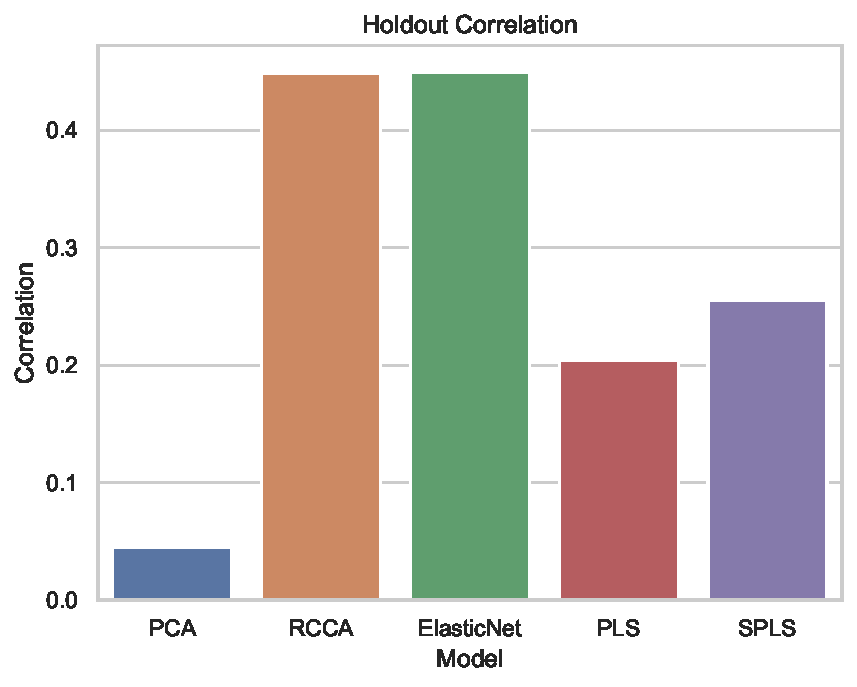
\includegraphics[width=0.5\linewidth]{figures/regularization/hcp/holdout_correlations.pdf}
\caption{Out-of-sample canonical correlations for each model.}\label{fig:performance}
\end{figure}

\subsubsection{Behaviour Weights and Loadings}

In this section, we plot the top 8 positive and negative non-imaging weights and loadings for each model.
This is to illustrate some of the effects we have observed in the previous section.
PCA finds a mode of variation in the behavioural data that is positively correlated with psychiatric and life function tests and negatively correlated with a number of emotion and personality tests.
The RCCA and ElasticNet models find a mode of variation in the behavioural data that is negatively correlated with the Line Orientation test and to a lesser extent smoking and positively correlated with a number of other cognitive tests.
The PLS model finds a mode of variation in the behavioural data that is somewhat similar to the `good-bad' mode in \cite{smith2015positive} with a positive correlation with agreeableness, vocabulary tests, and feelings about ones life and a strong negative correlation with smoking, rule-breaking, and antisocial personality traits.
The SPLS mode is similar but selects out the rule-breaking and antisocial personality traits in favour of the vocabulary tests and smoking.

\begin{figure}
\centering
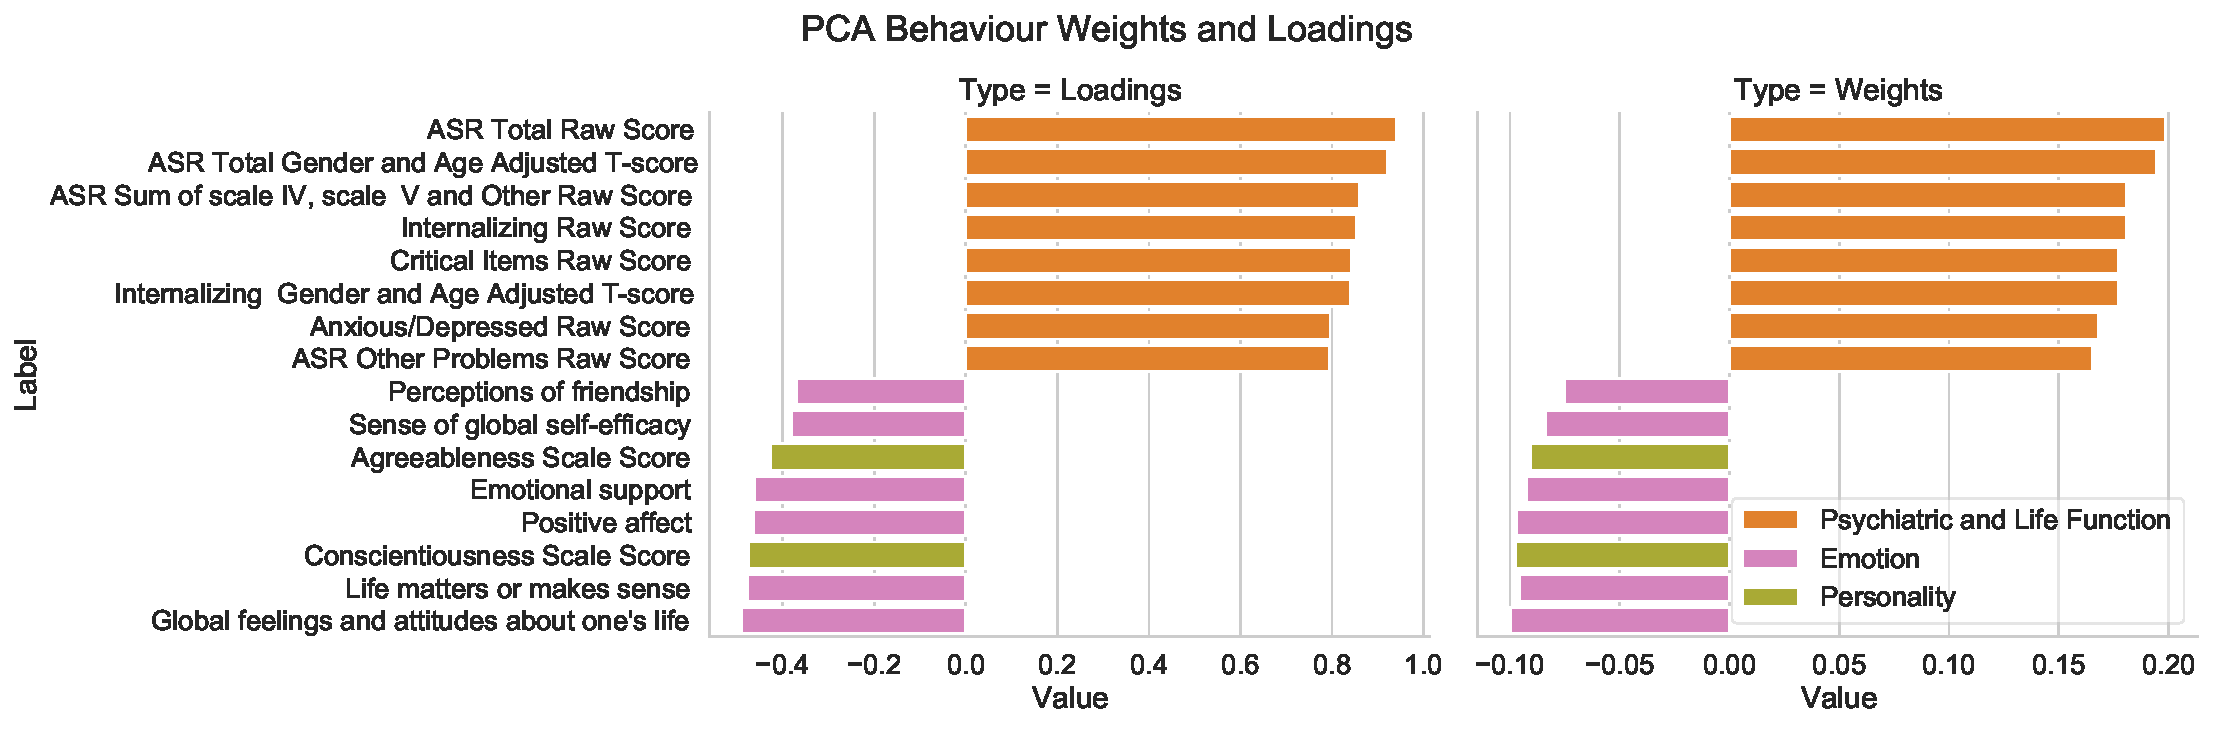
\includegraphics[width=0.8\linewidth]{figures/regularization/hcp/PCA behaviour weights and loadings.pdf}
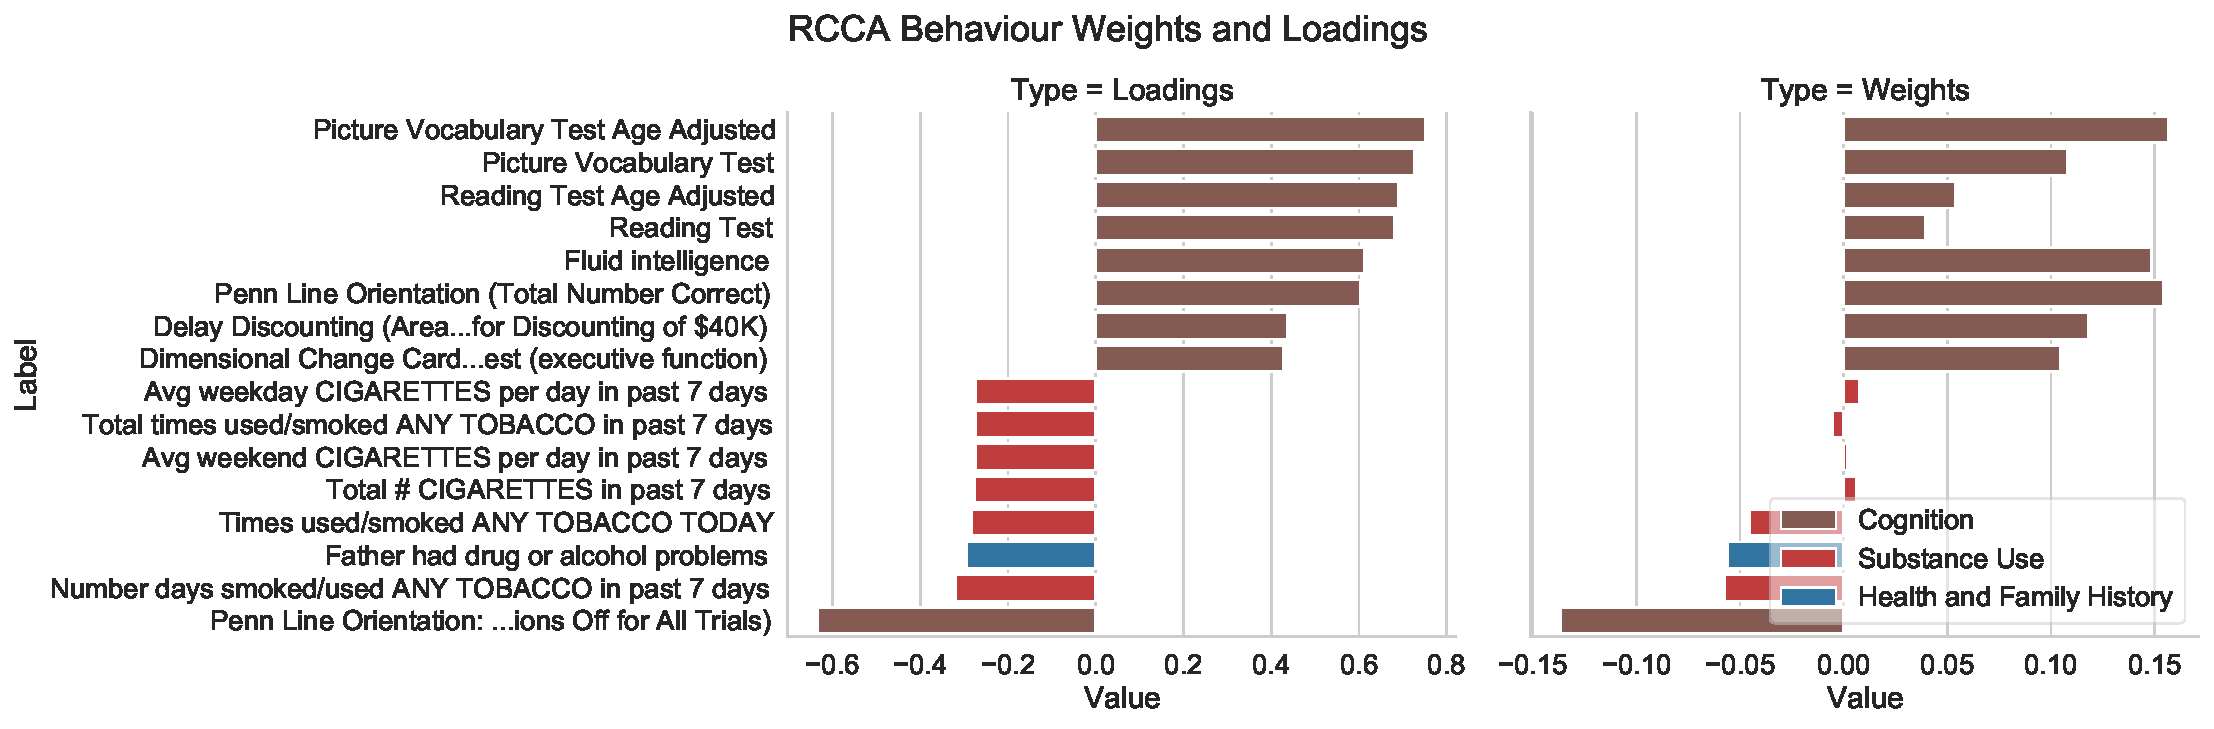
\includegraphics[width=0.8\linewidth]{figures/regularization/hcp/RCCA behaviour weights and loadings.pdf}
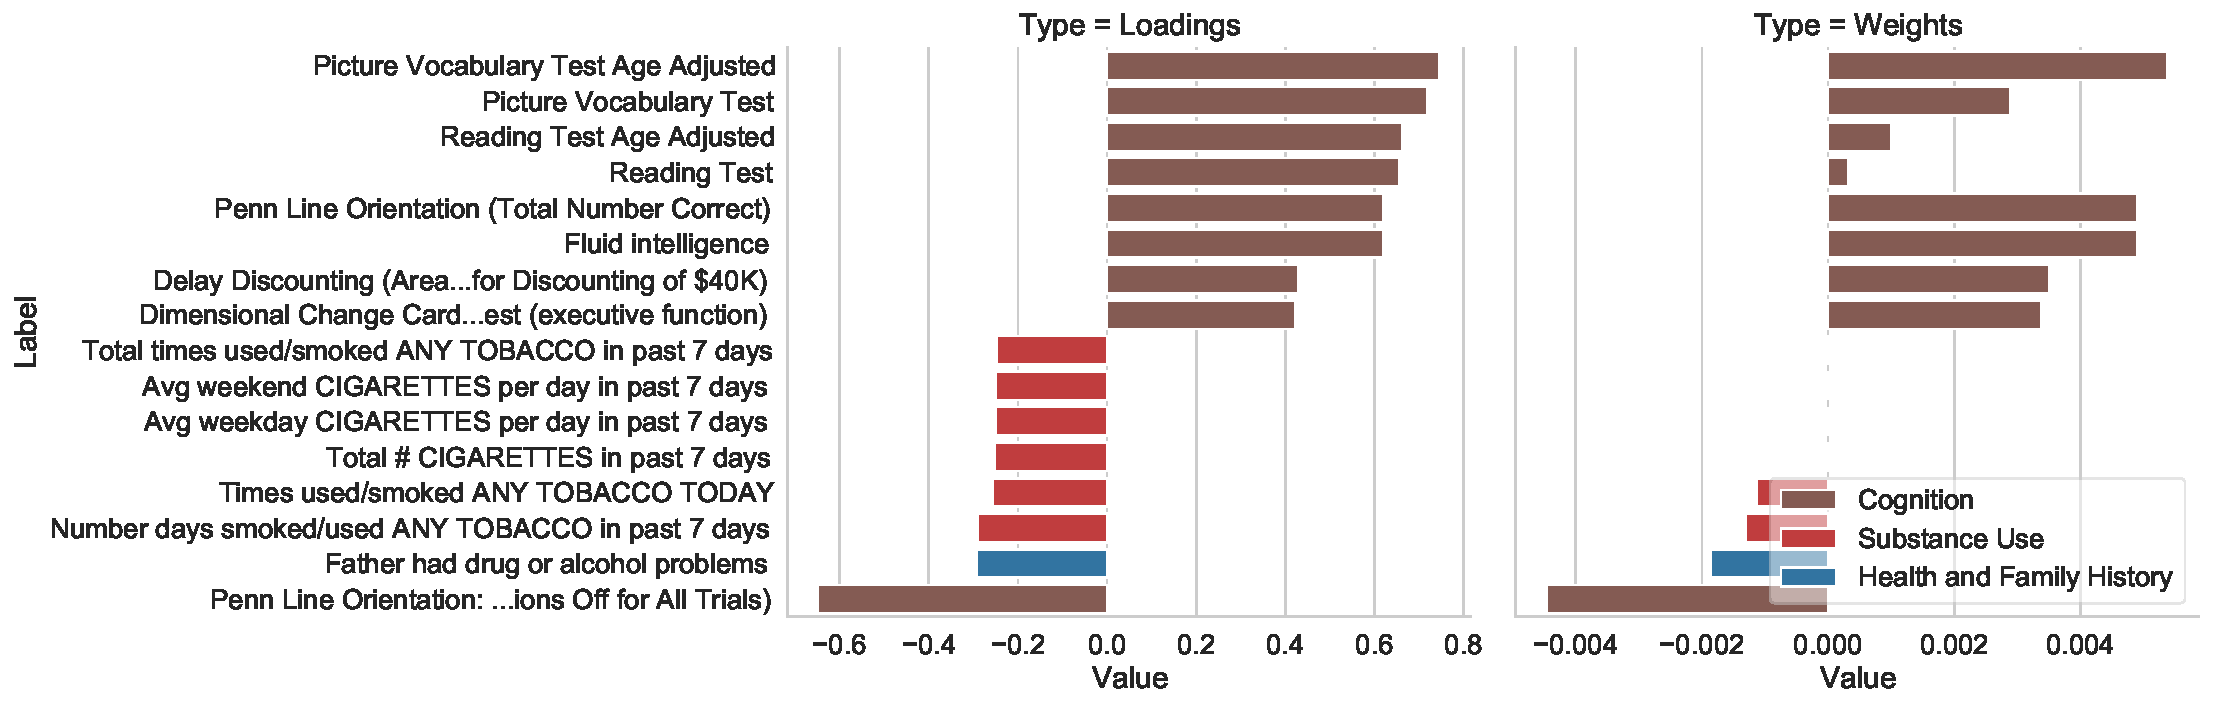
\includegraphics[width=0.8\linewidth]{figures/regularization/hcp/ElasticNet behaviour weights and loadings.pdf}
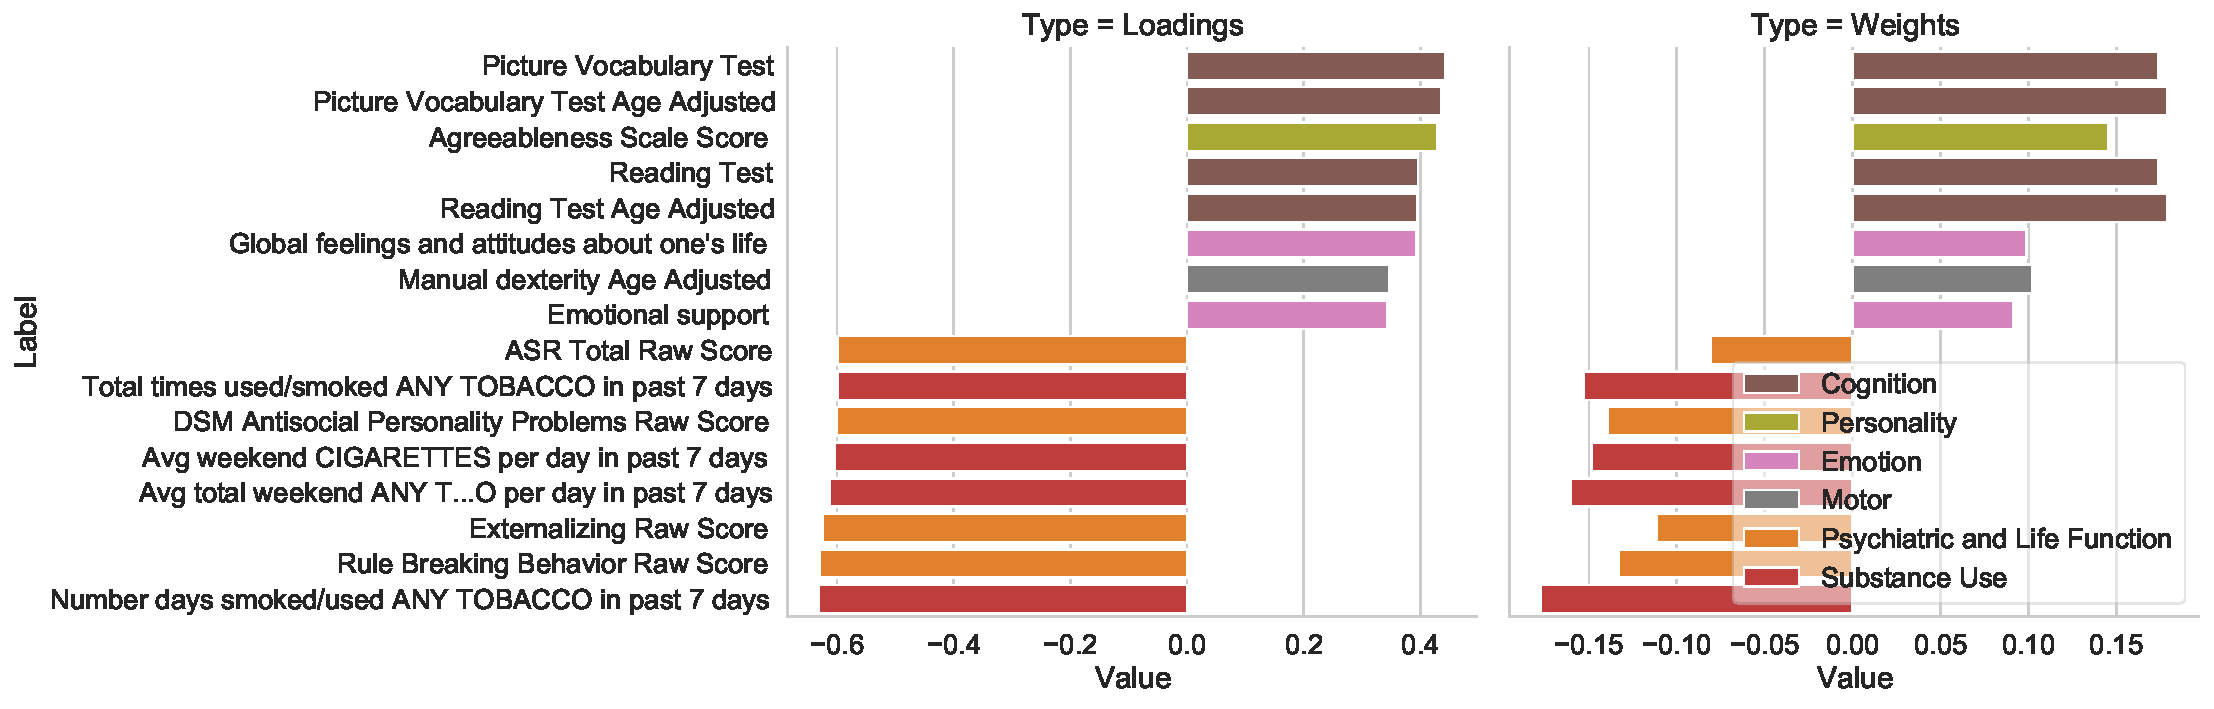
\includegraphics[width=0.8\linewidth]{figures/regularization/hcp/PLS behaviour weights and loadings.pdf}
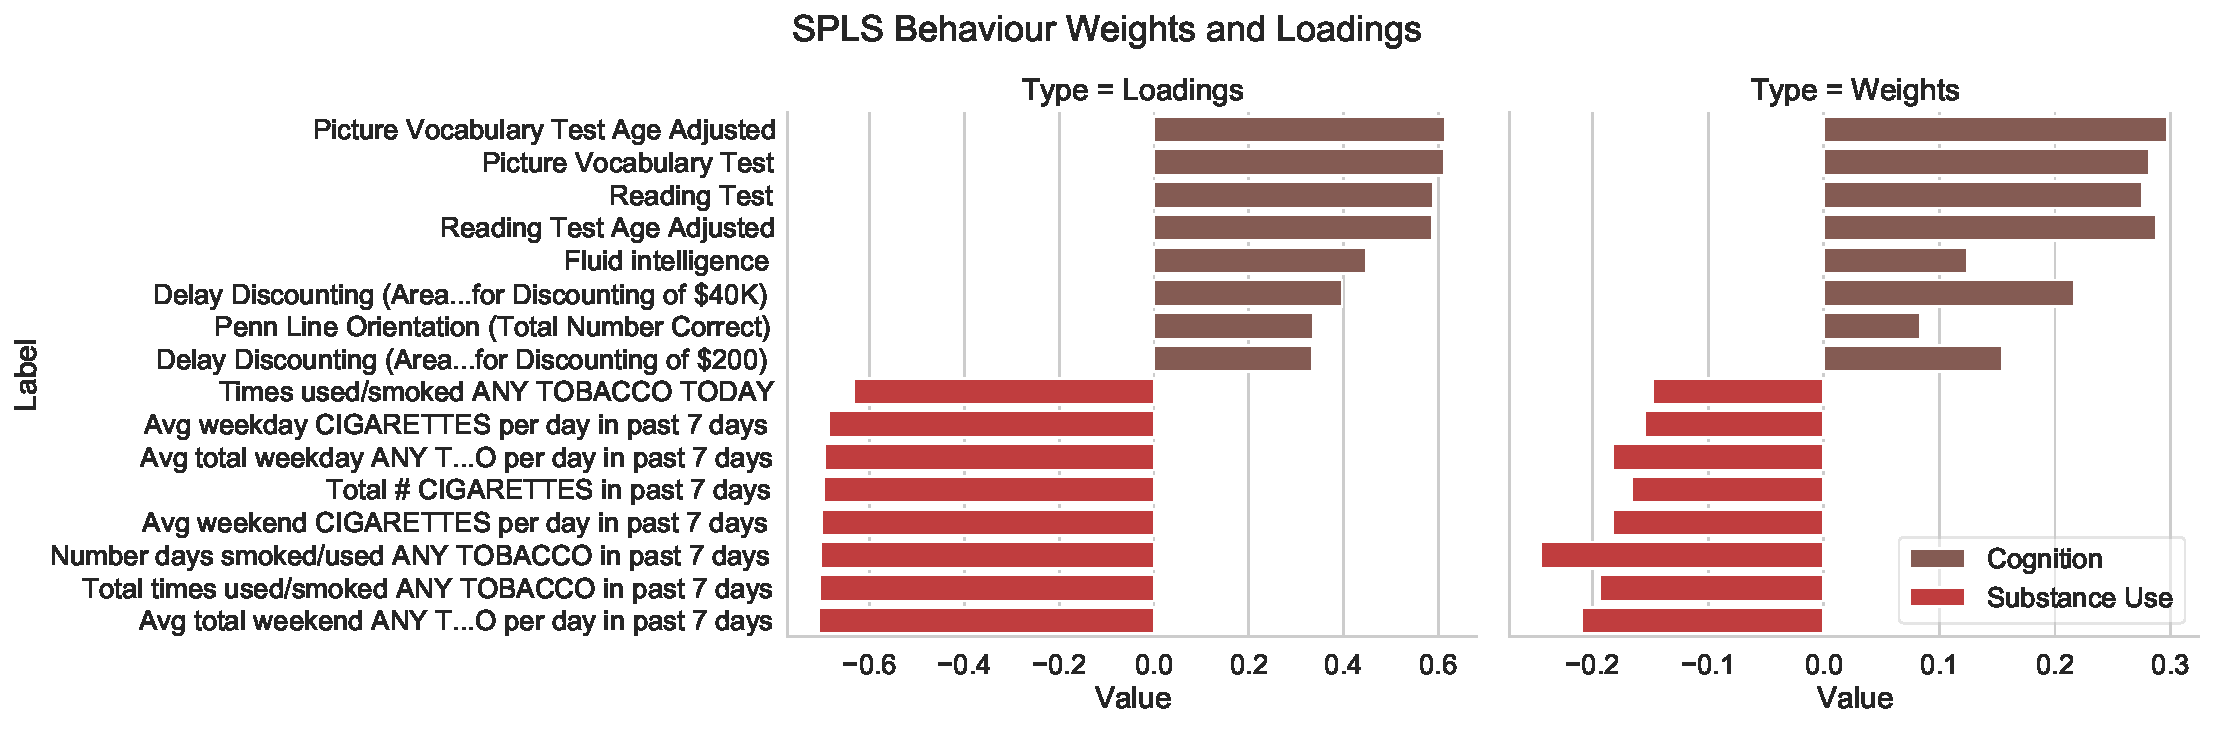
\includegraphics[width=0.8\linewidth]{figures/regularization/hcp/SPLS behaviour weights and loadings.pdf}
\caption{Top 8 positive and negative non-imaging loadings for each model}\label{fig:behaviour}
\end{figure}

\subsubsection{Connectivity Weights}
\begin{figure}
\centering
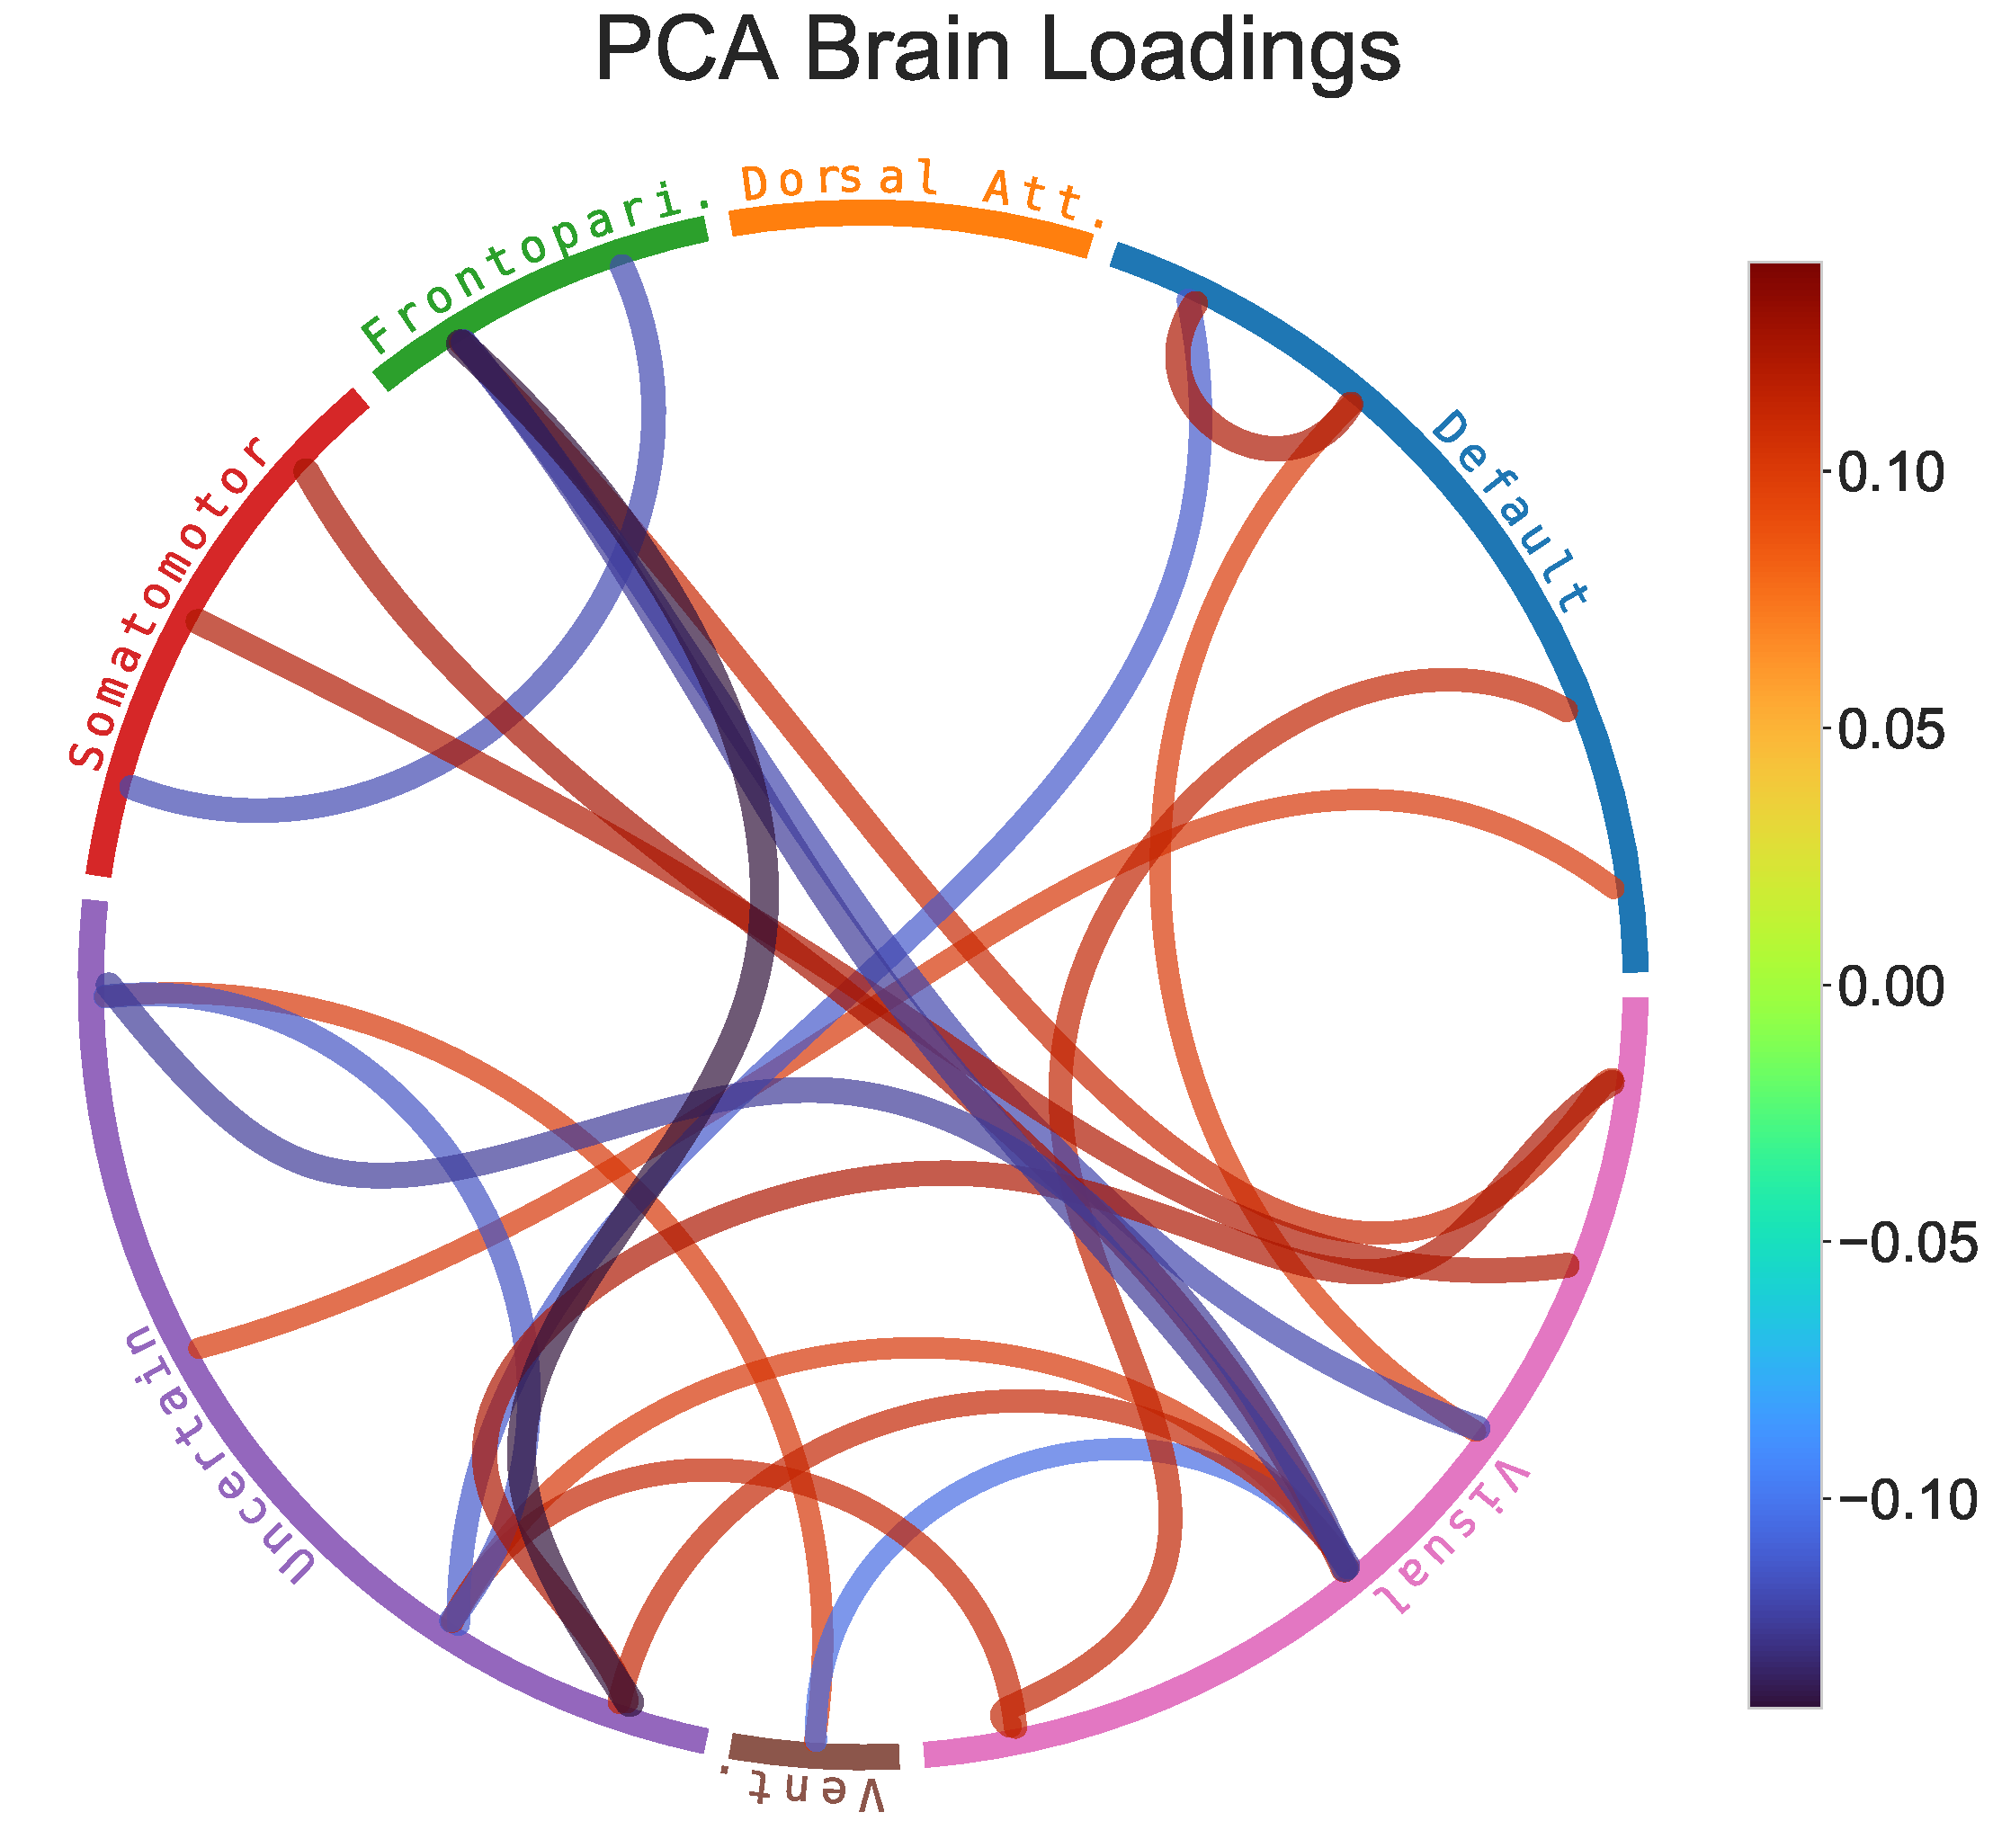
\includegraphics[width=0.49\linewidth]{figures/regularization/hcp/PCA brain weights.pdf}
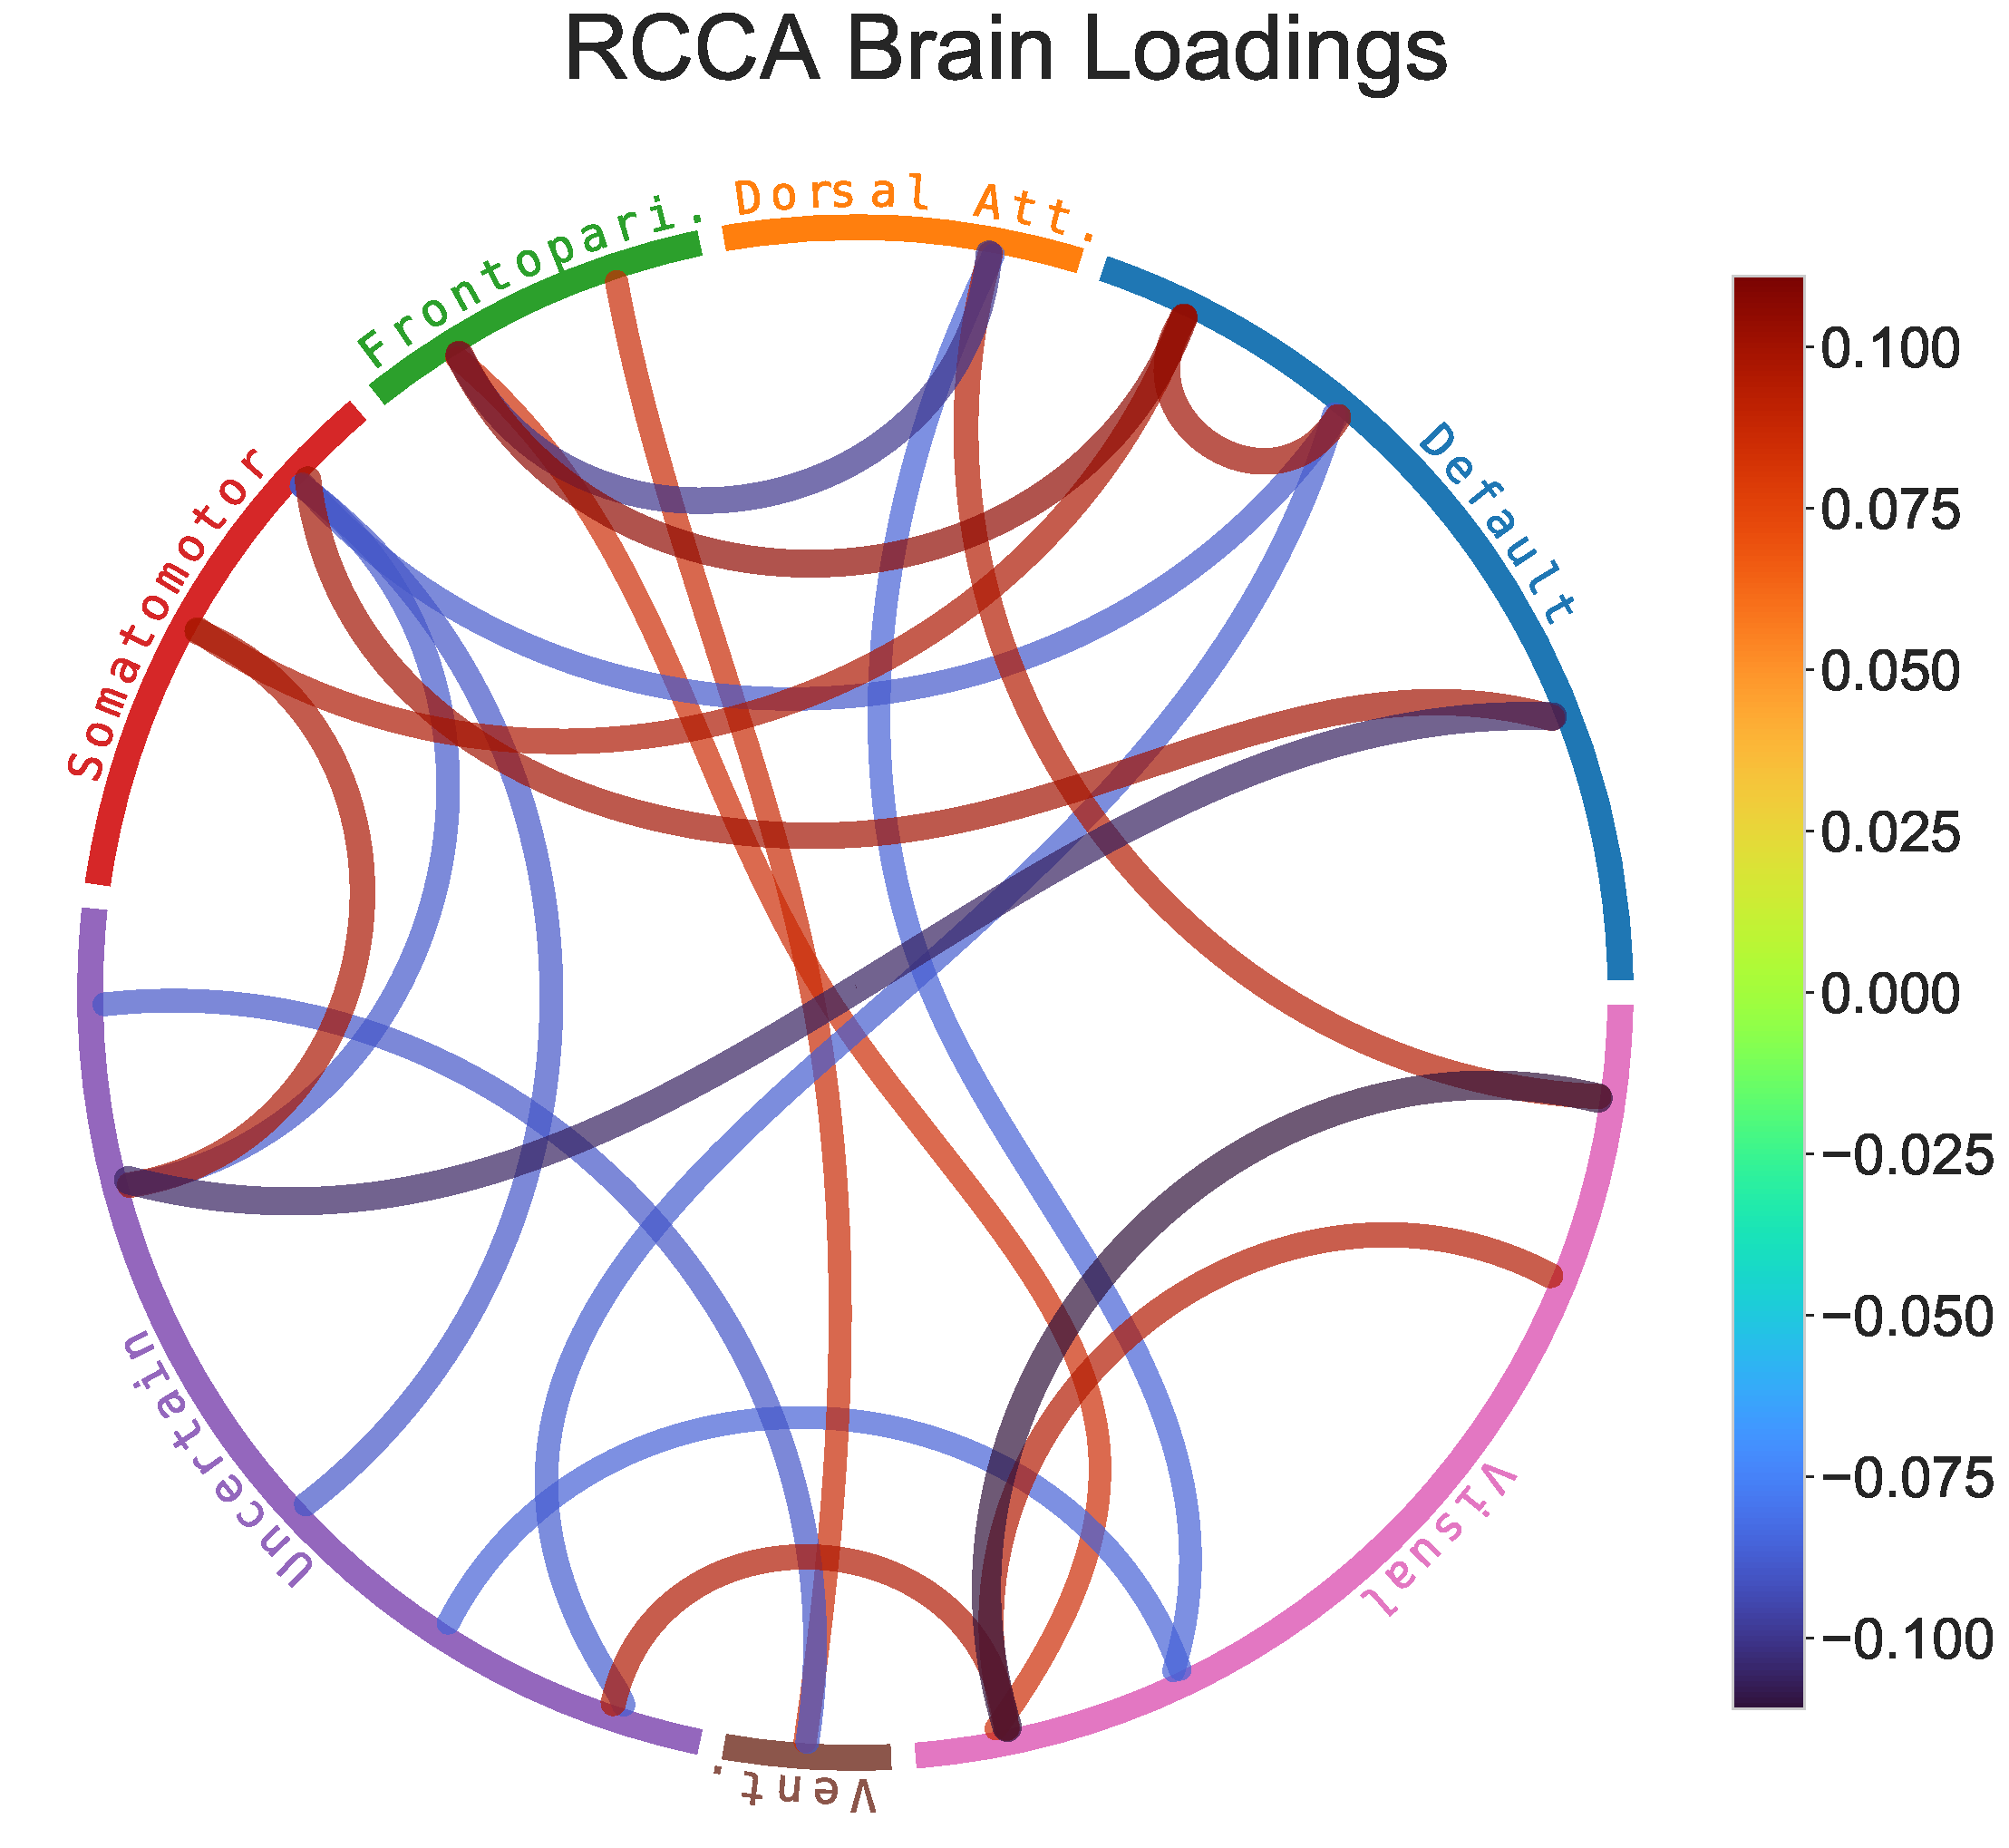
\includegraphics[width=0.49\linewidth]{figures/regularization/hcp/RCCA brain weights.pdf}
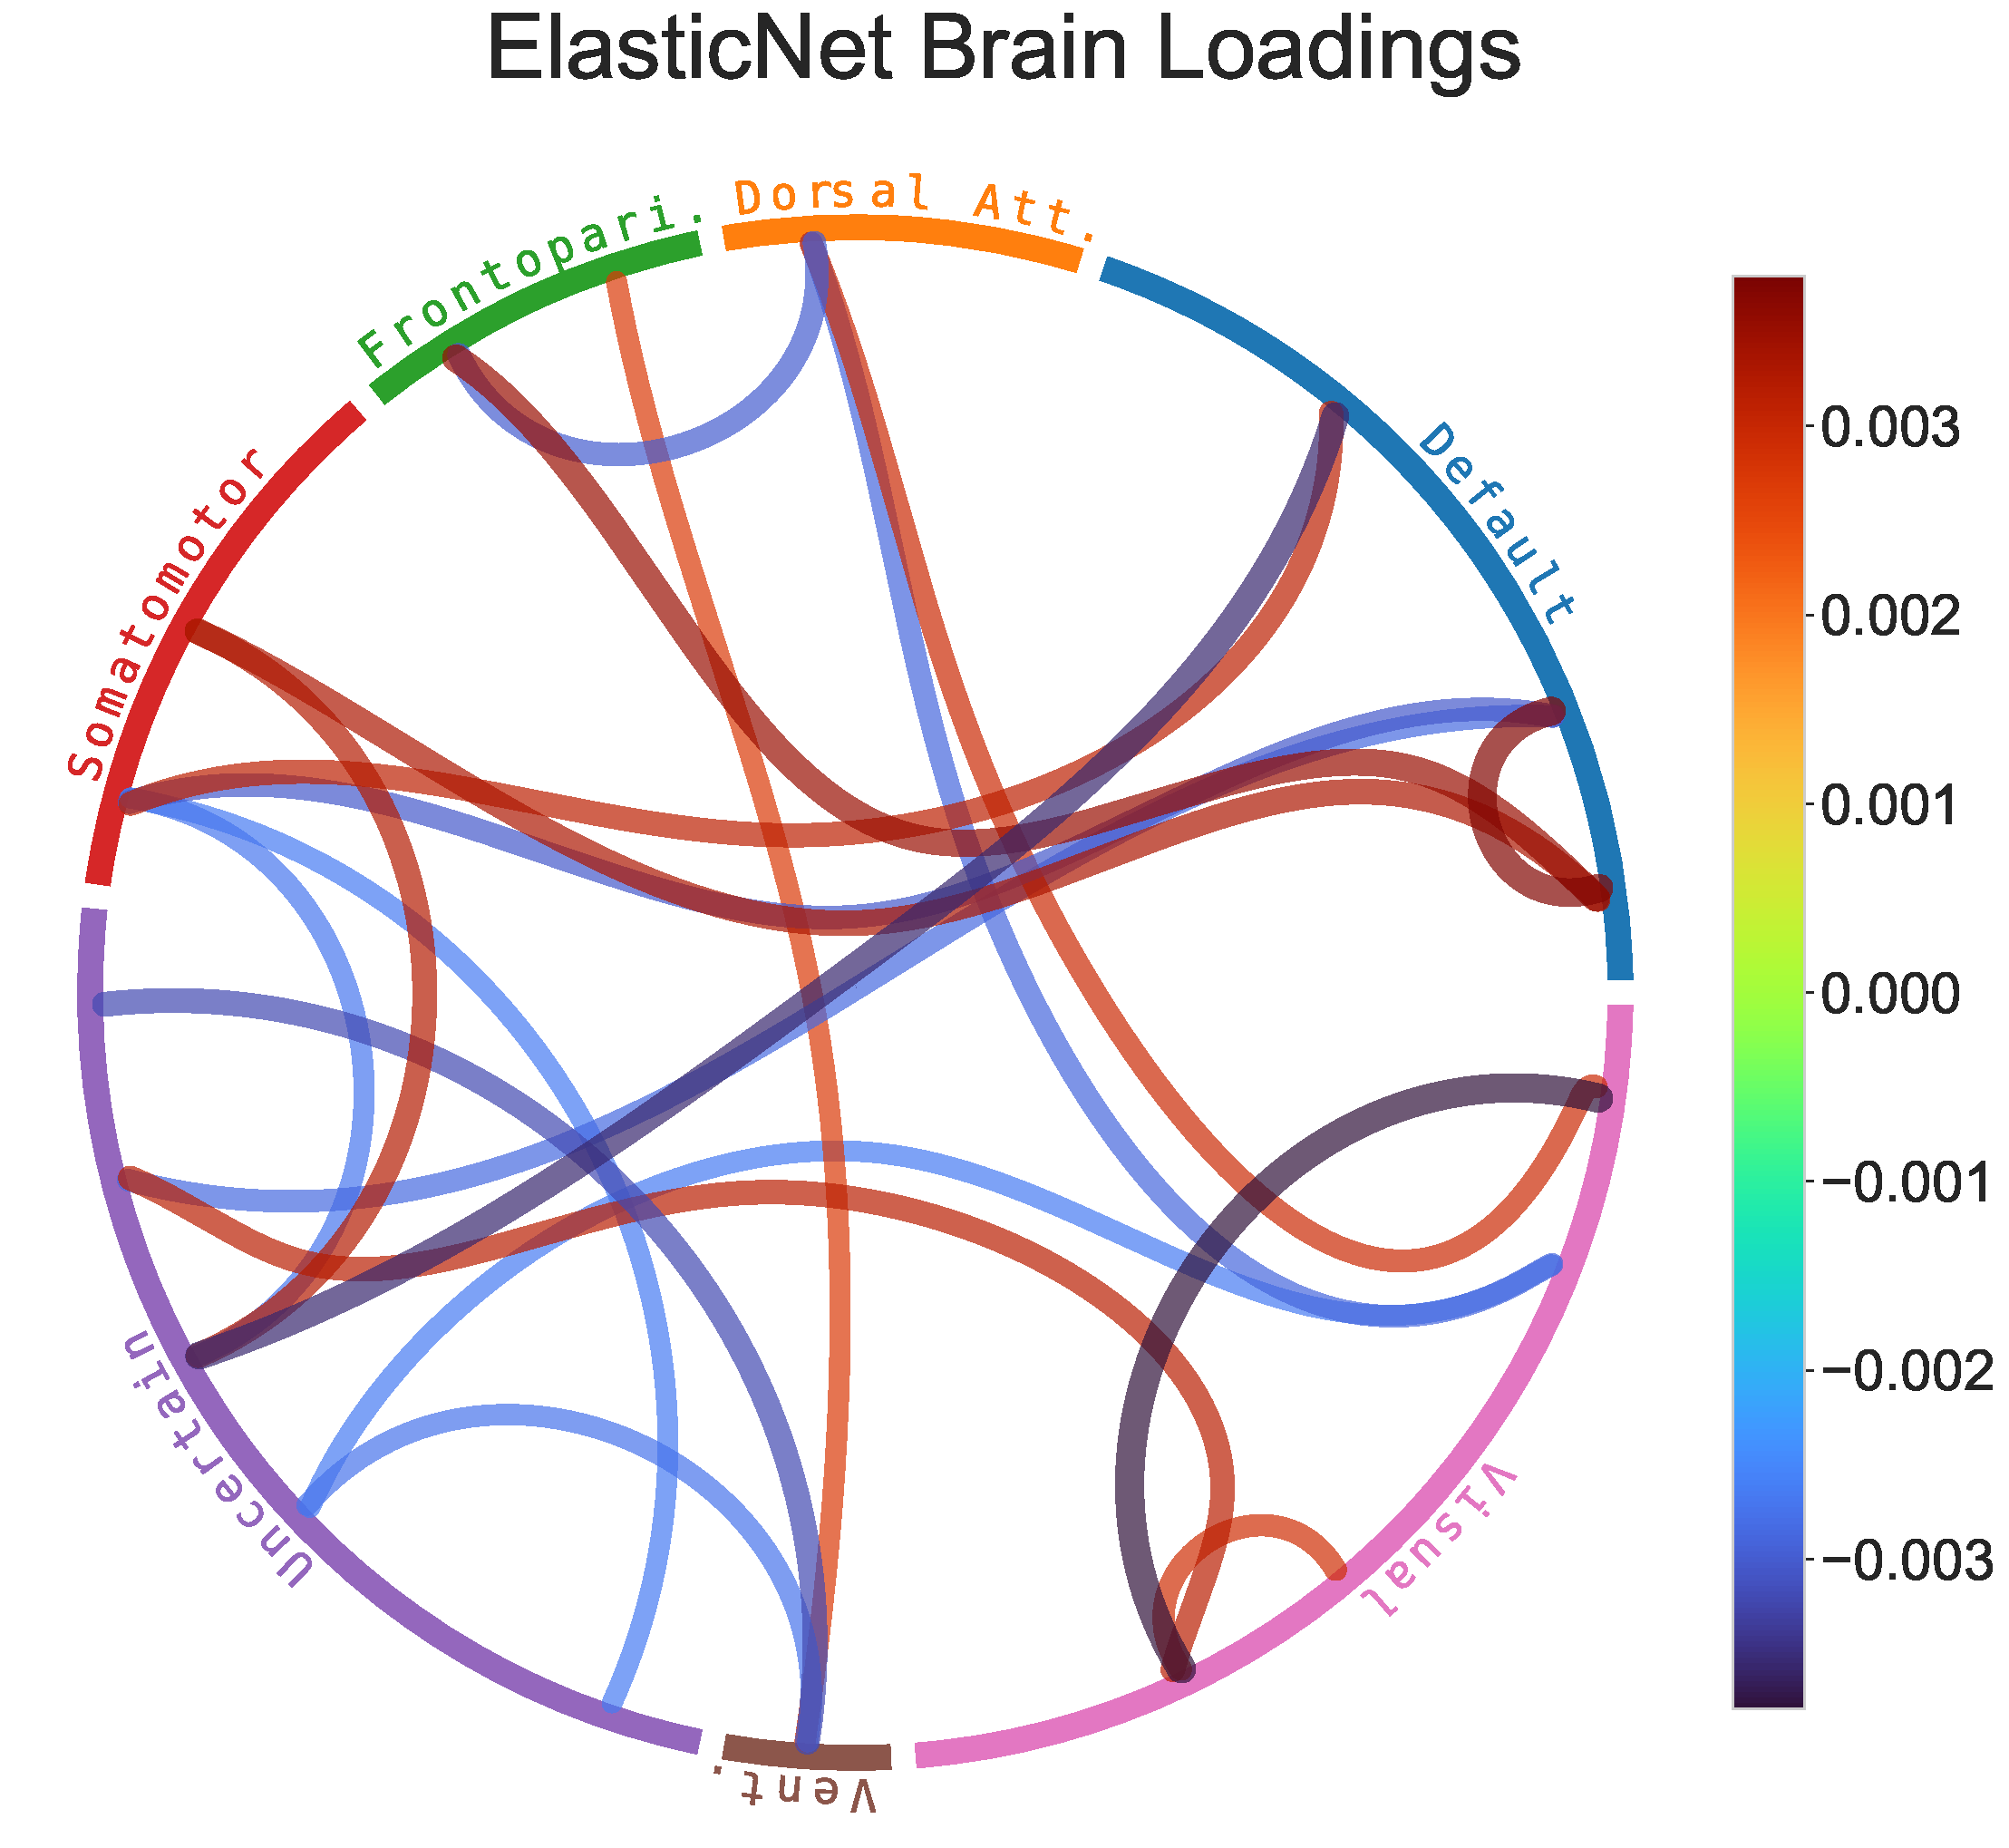
\includegraphics[width=0.49\linewidth]{figures/regularization/hcp/ElasticNet brain weights.pdf}
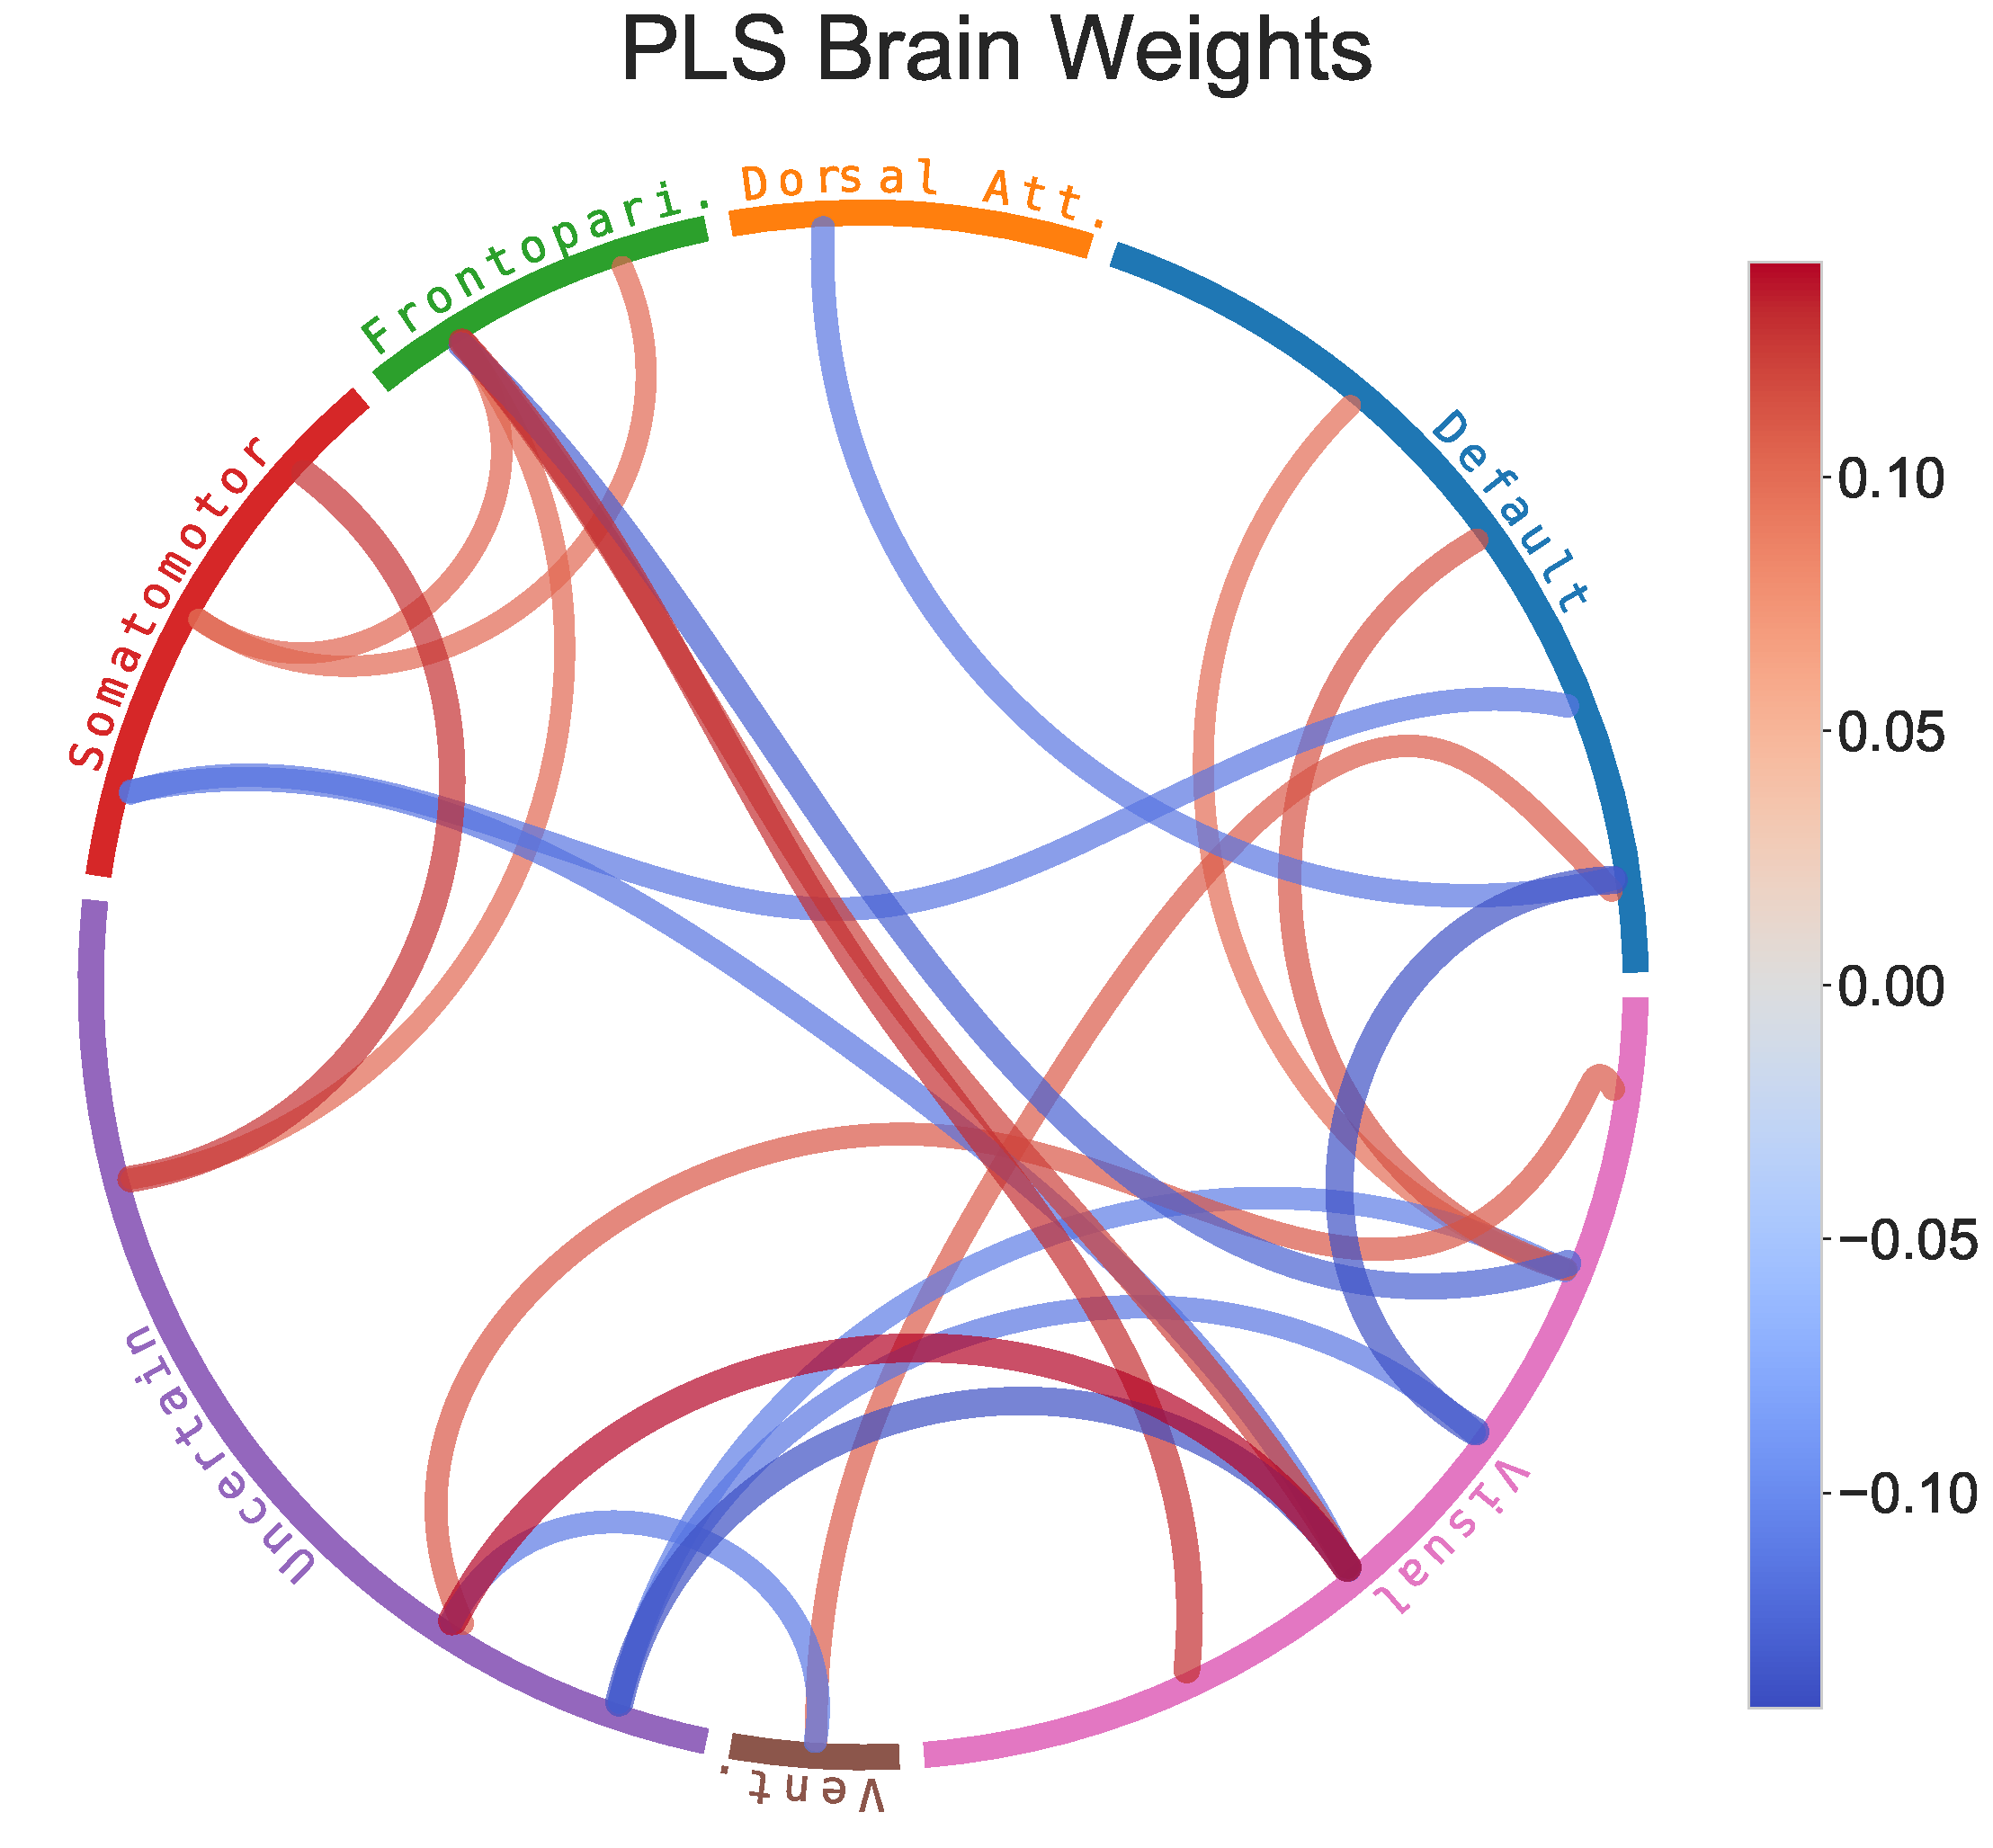
\includegraphics[width=0.49\linewidth]{figures/regularization/hcp/PLS brain weights.pdf}
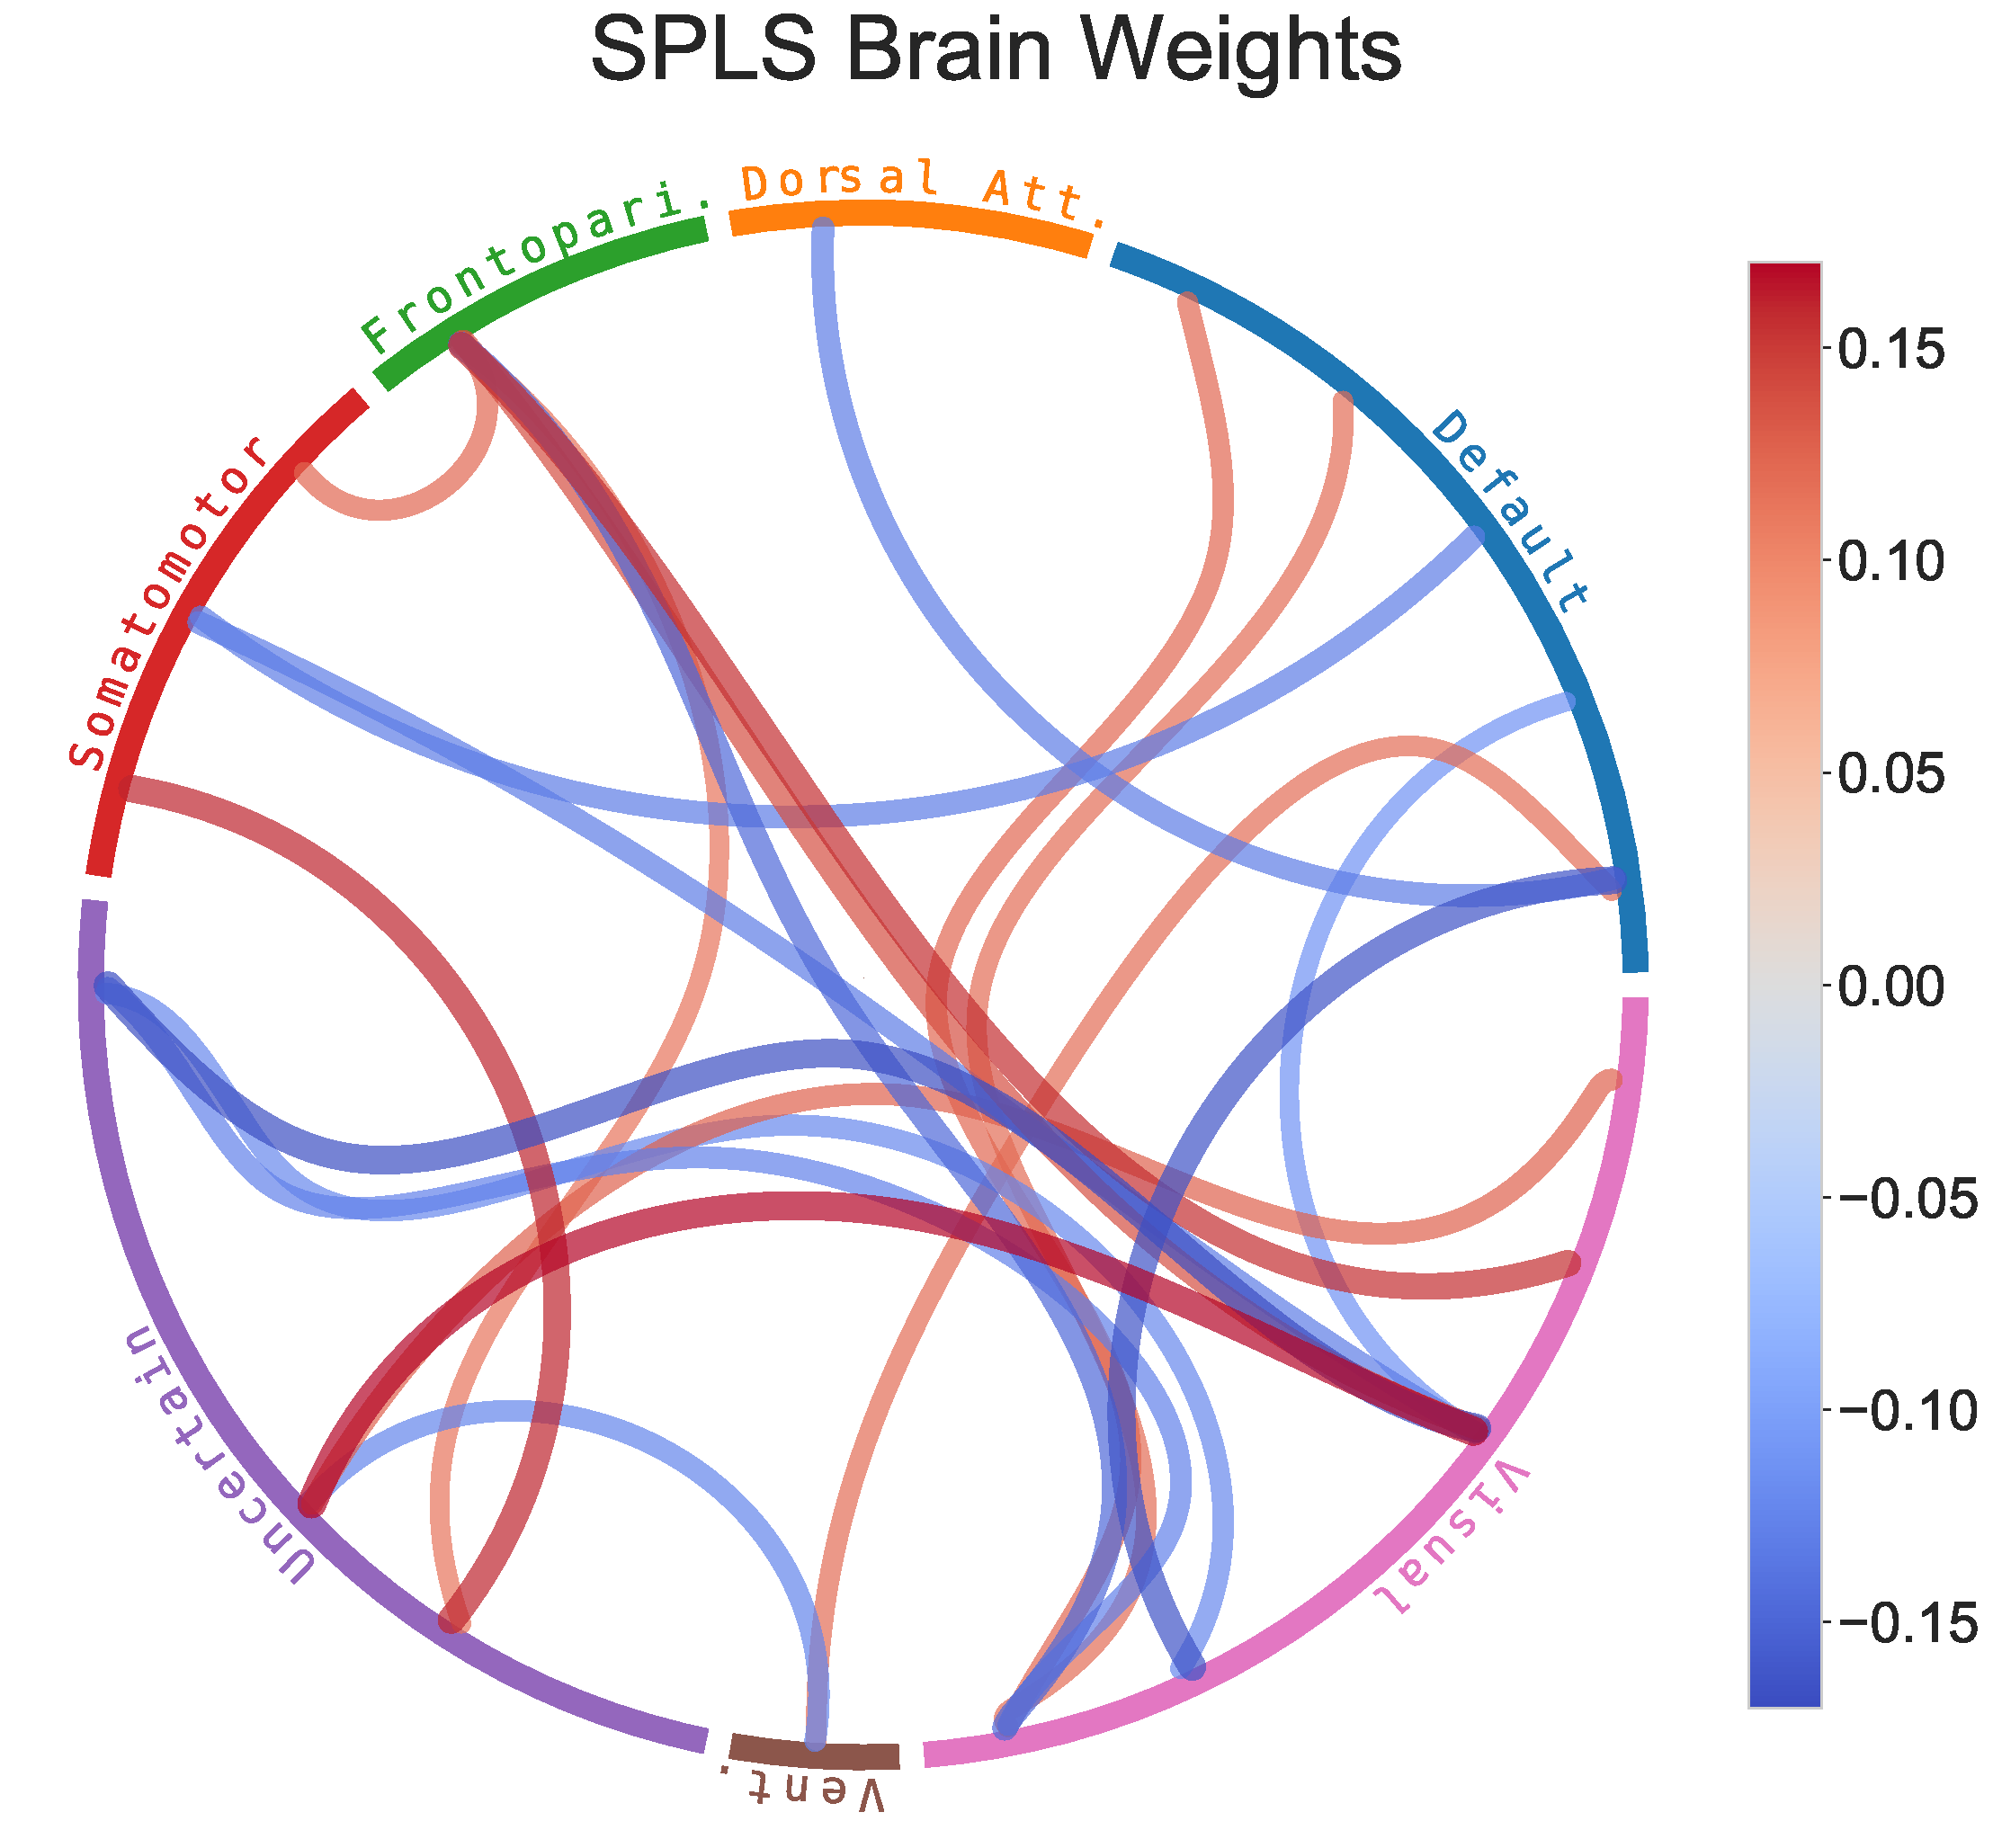
\includegraphics[width=0.49\linewidth]{figures/regularization/hcp/SPLS brain weights.pdf}
\caption{}\label{}
\end{figure}

\subsubsection{Connectivity Loadings}
\begin{figure}
\centering
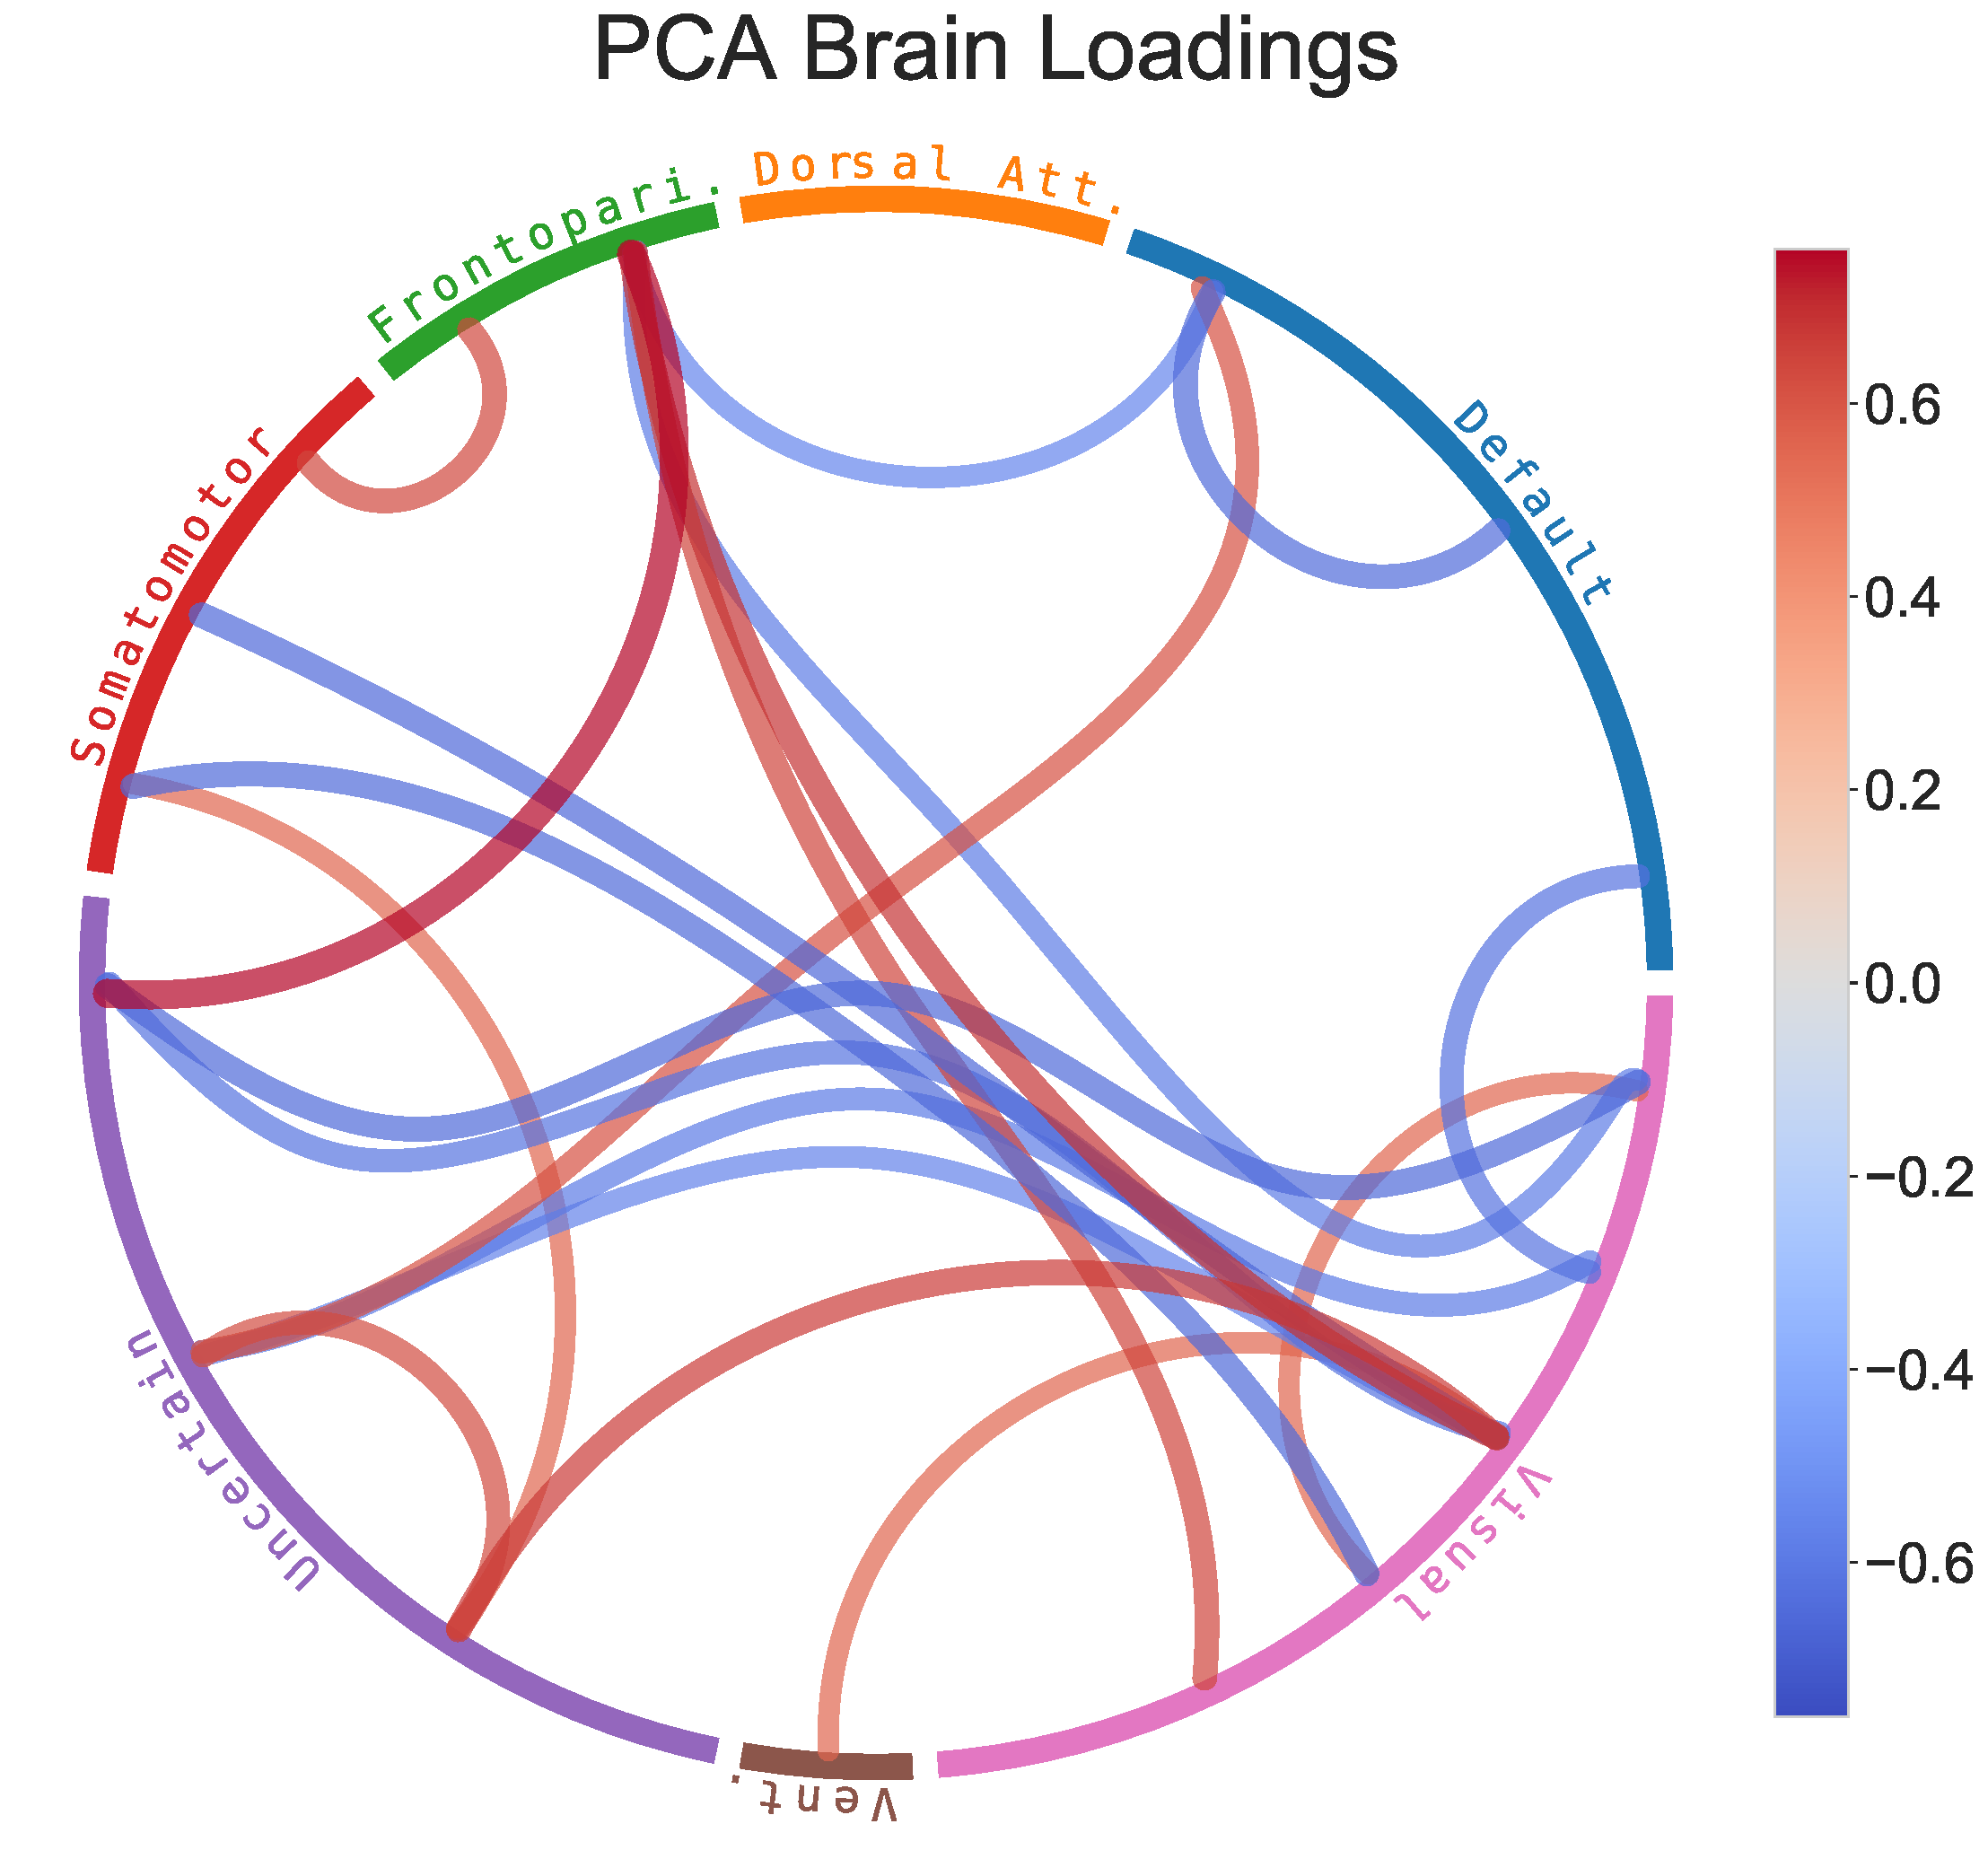
\includegraphics[width=0.49\linewidth]{figures/regularization/hcp/PCA brain loadings.pdf}
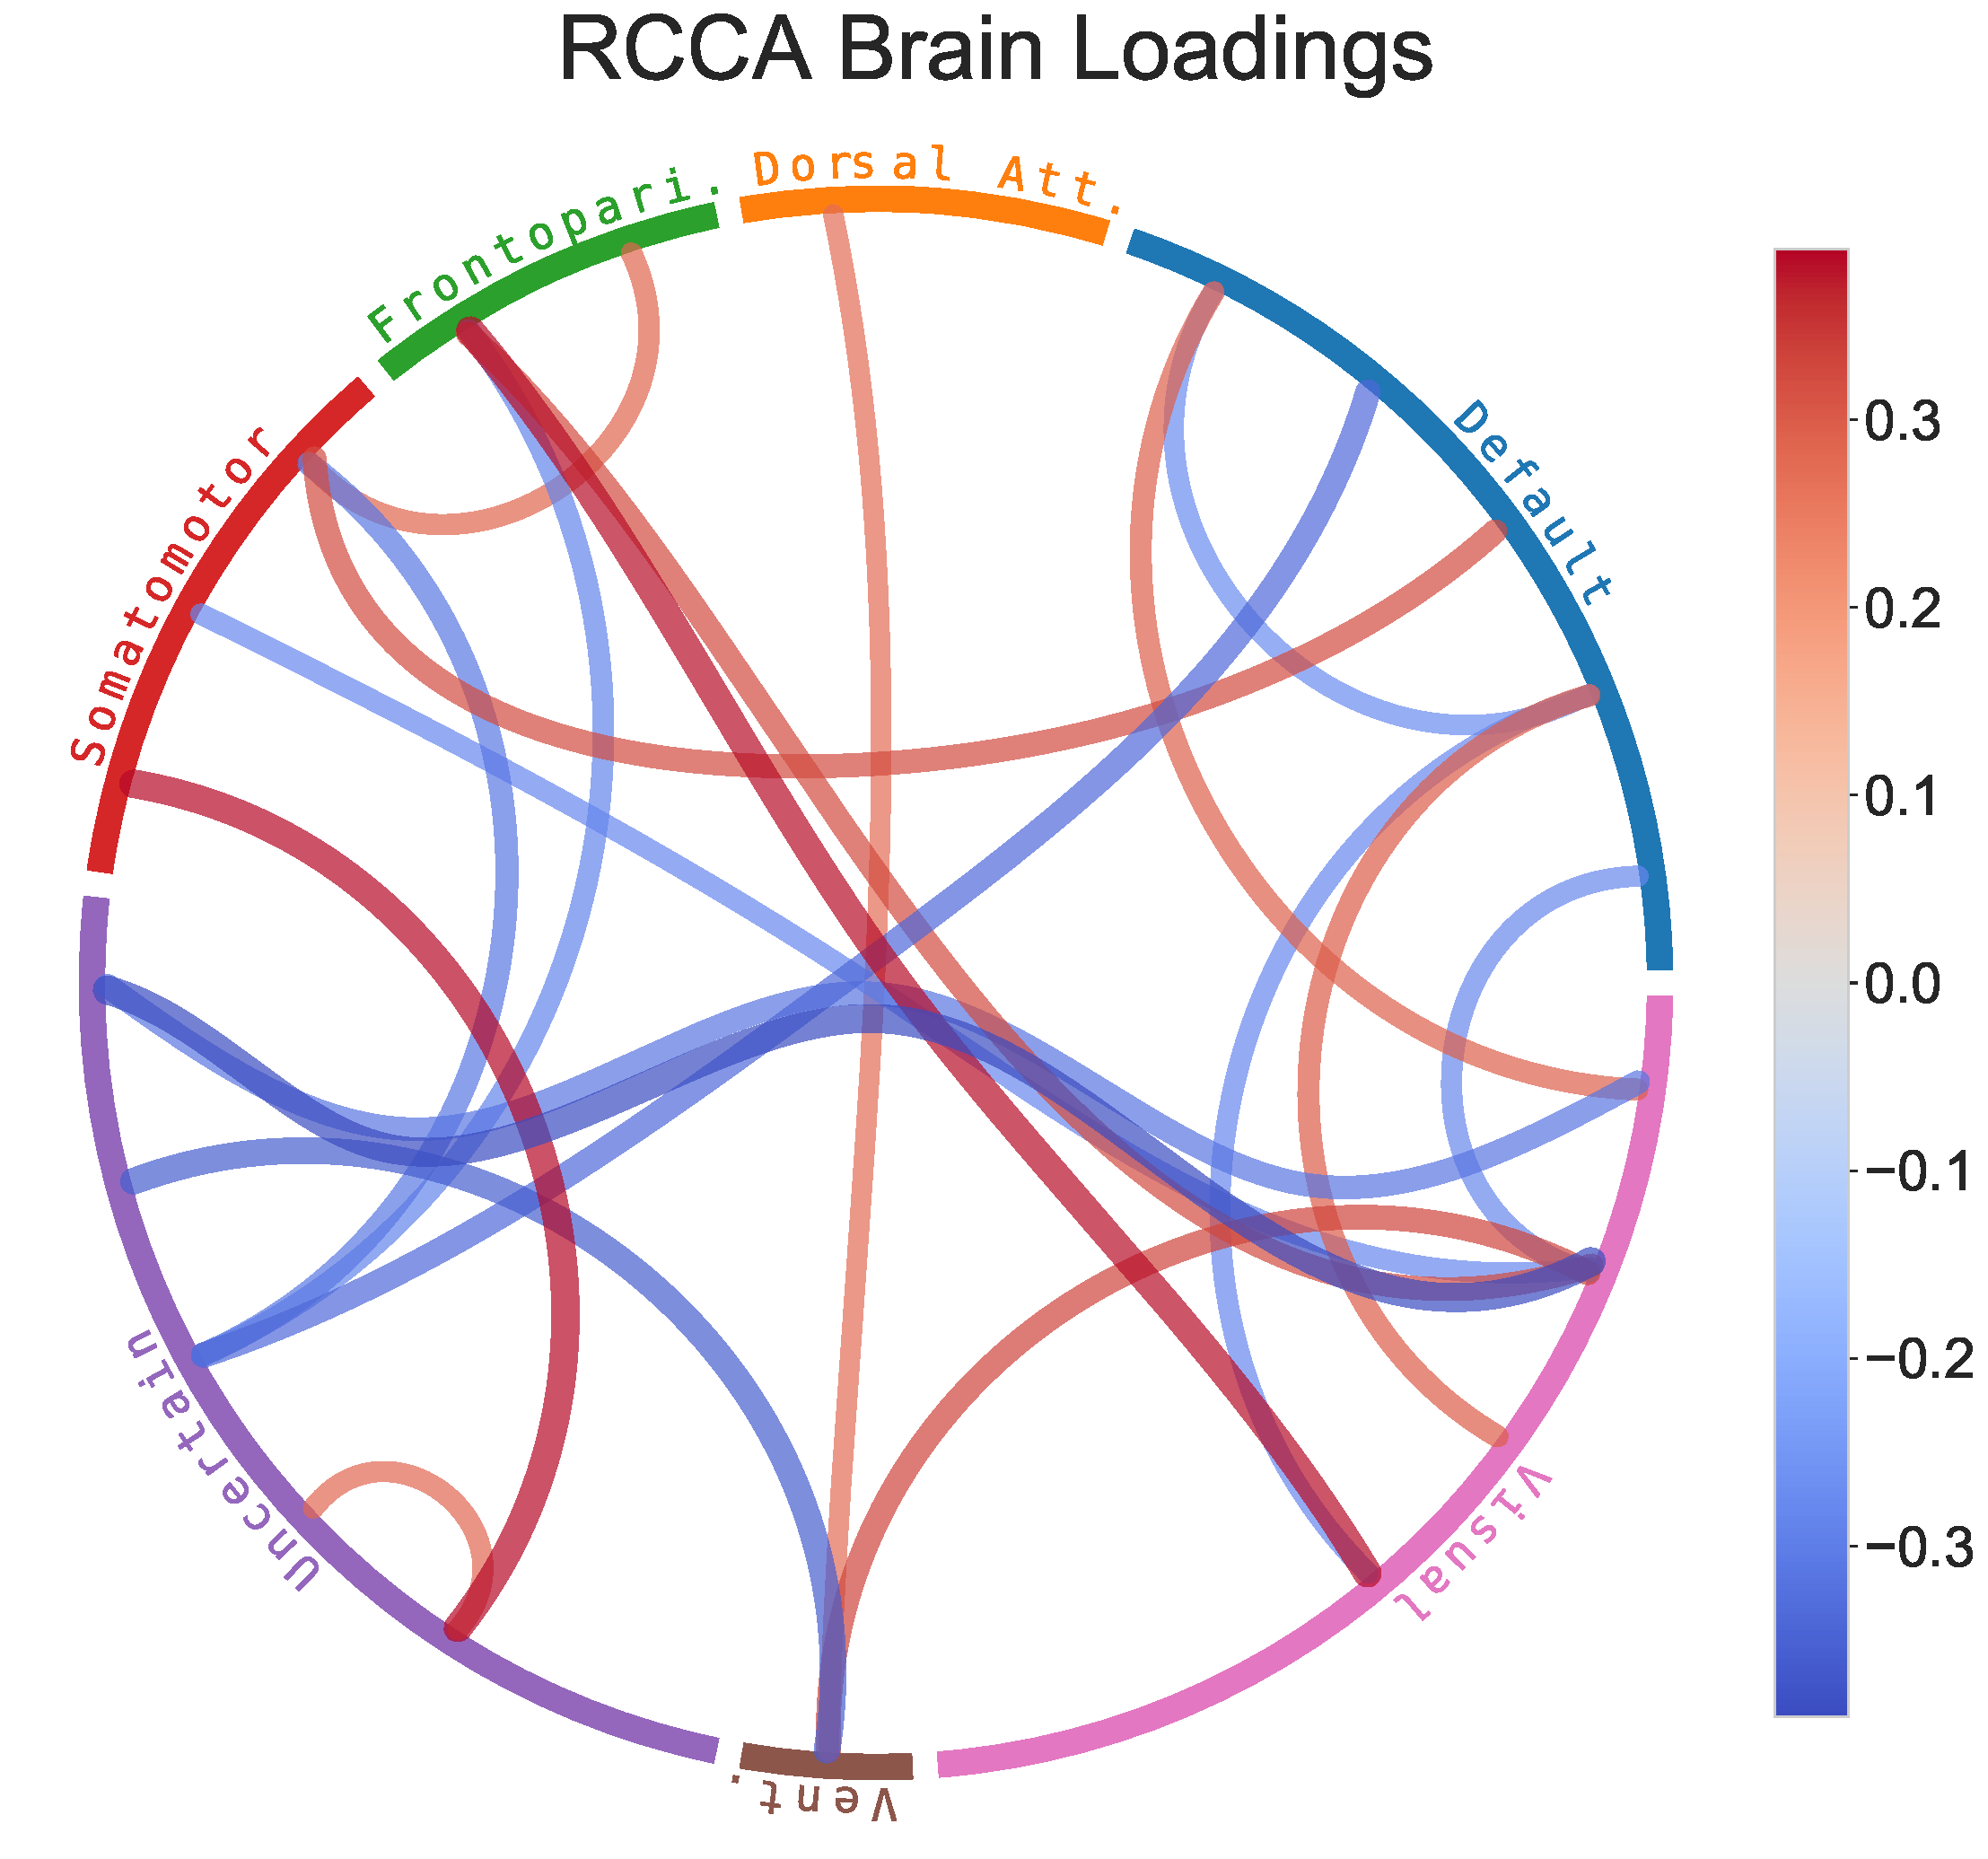
\includegraphics[width=0.49\linewidth]{figures/regularization/hcp/RCCA brain loadings.pdf}
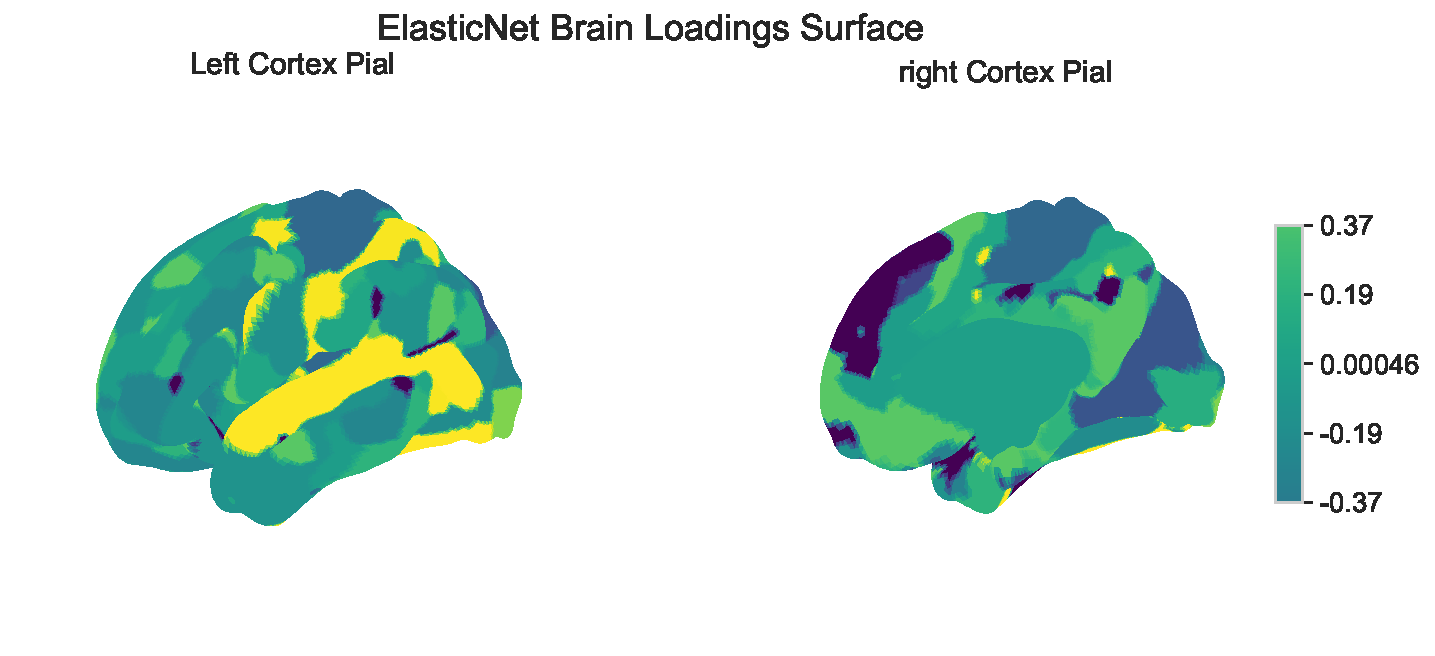
\includegraphics[width=0.49\linewidth]{figures/regularization/hcp/ElasticNet brain loadings.pdf}
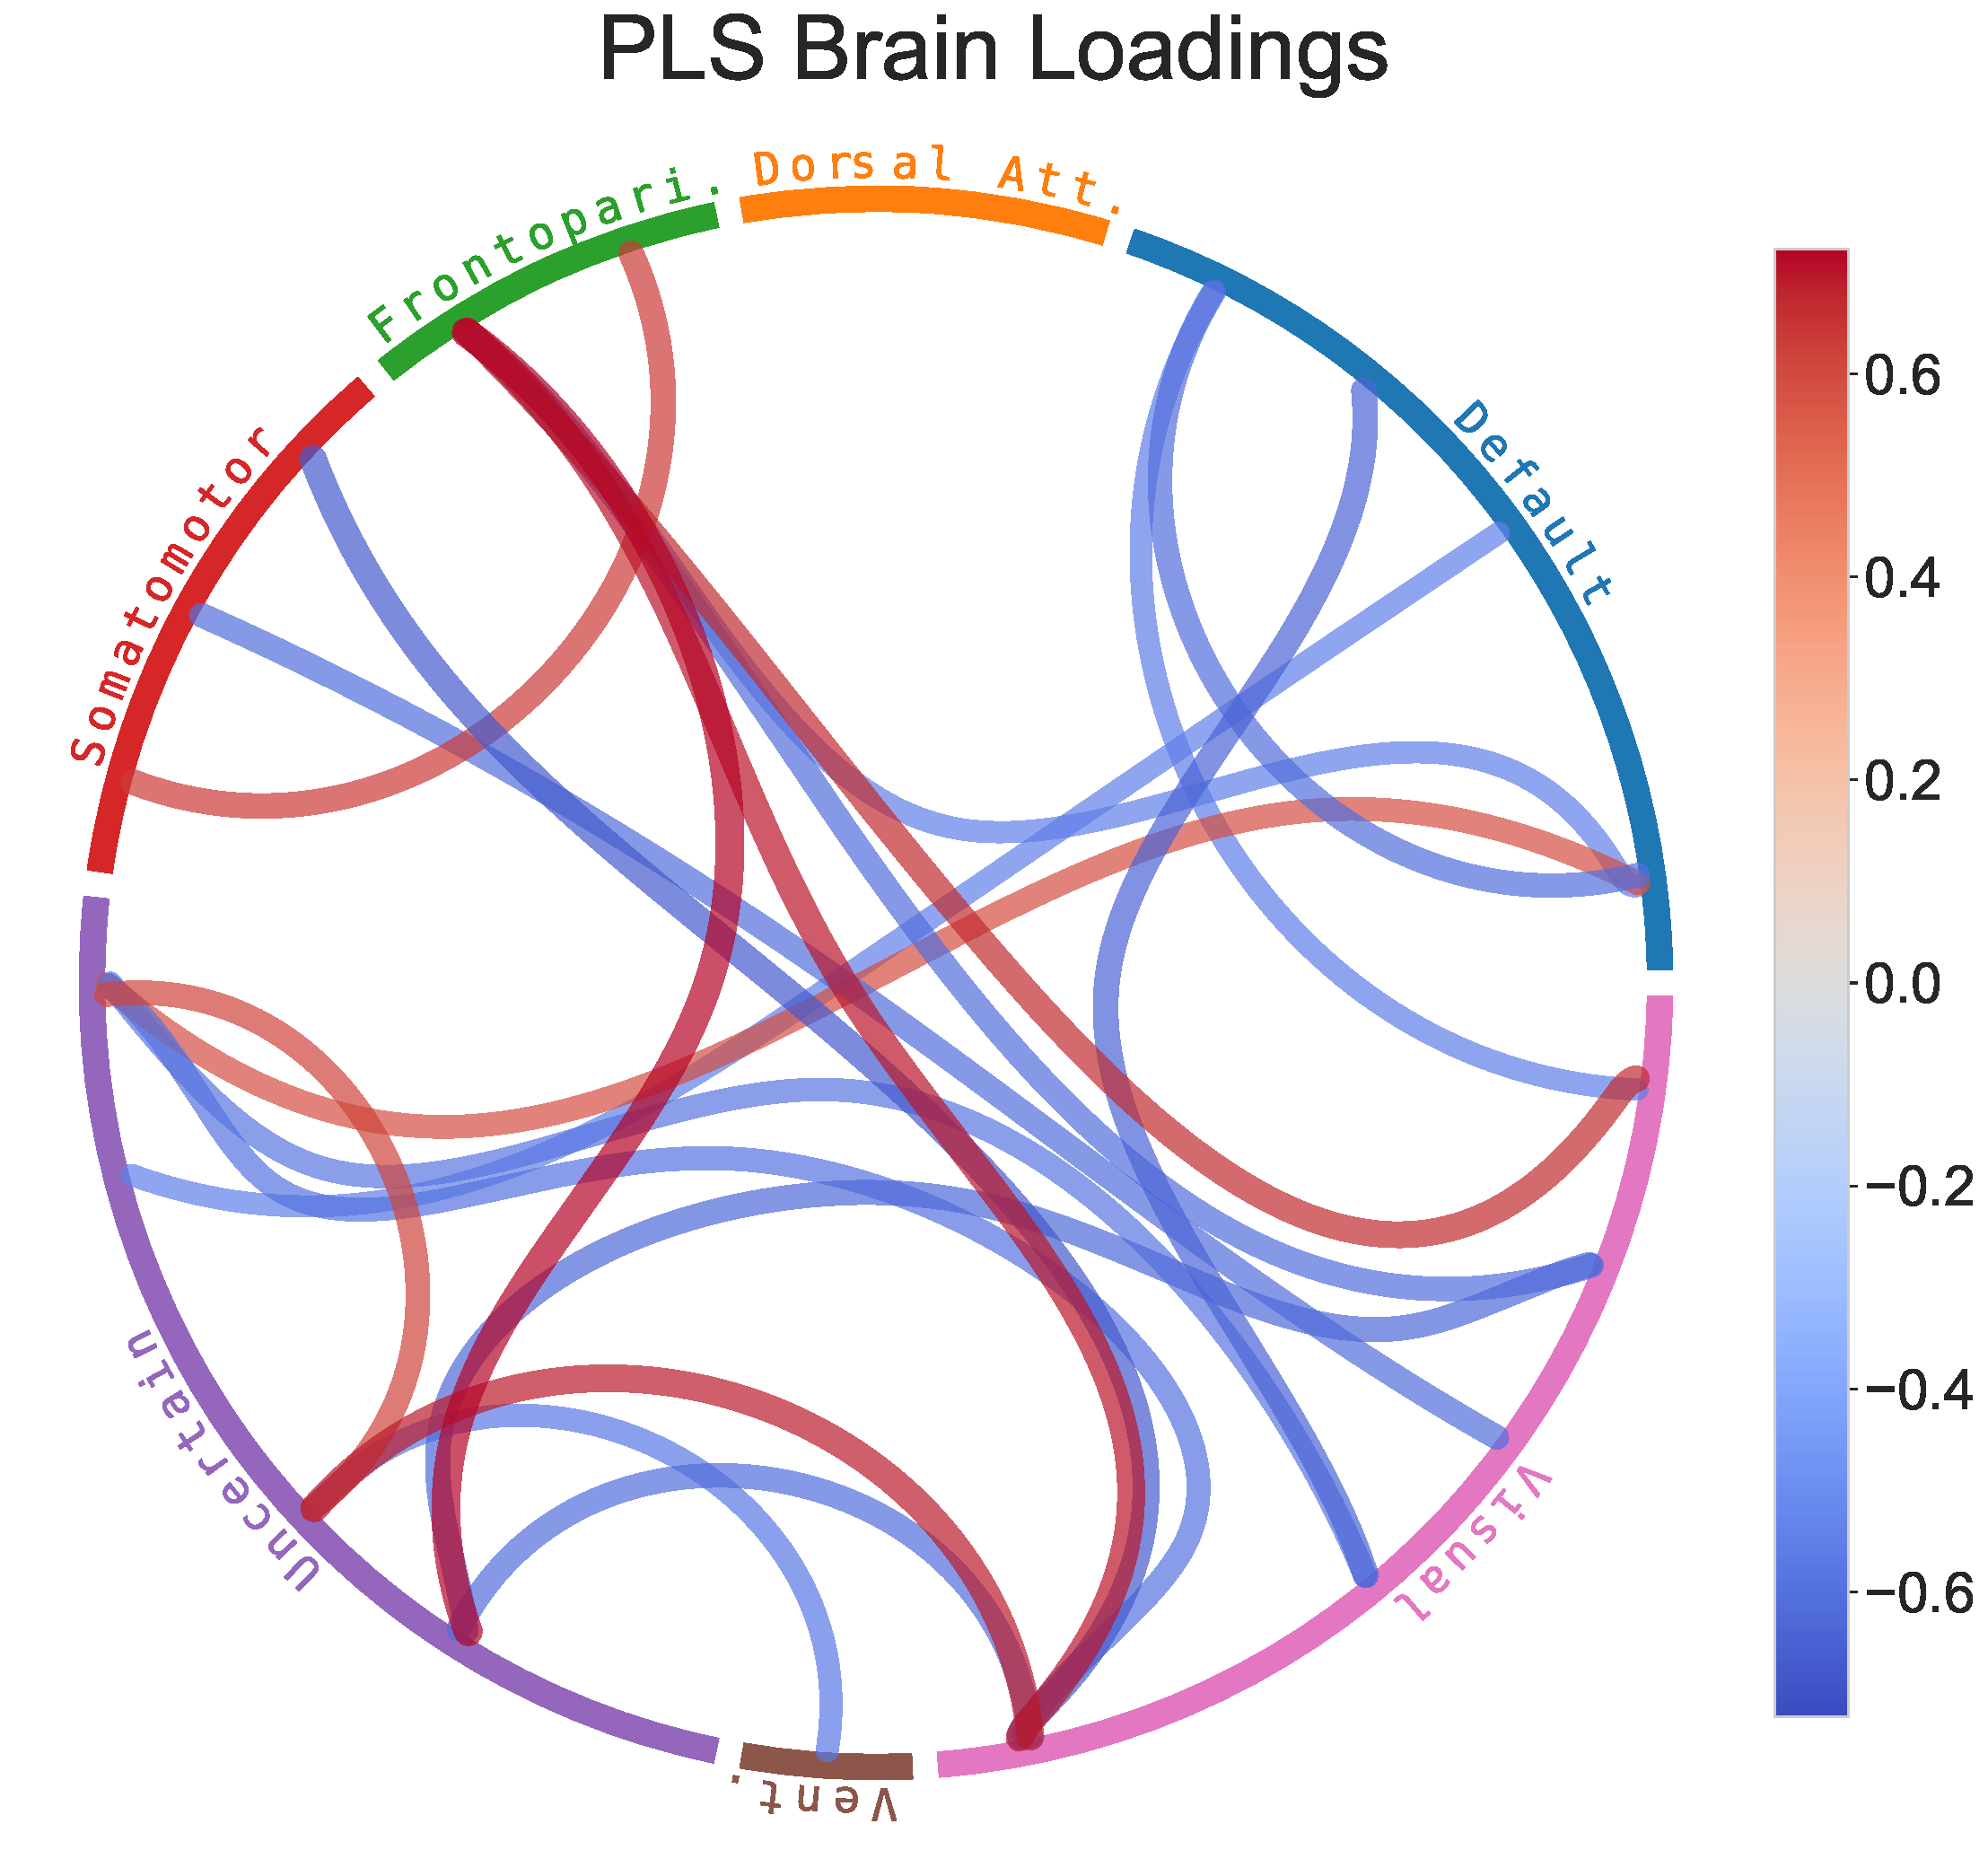
\includegraphics[width=0.49\linewidth]{figures/regularization/hcp/PLS brain loadings.pdf}
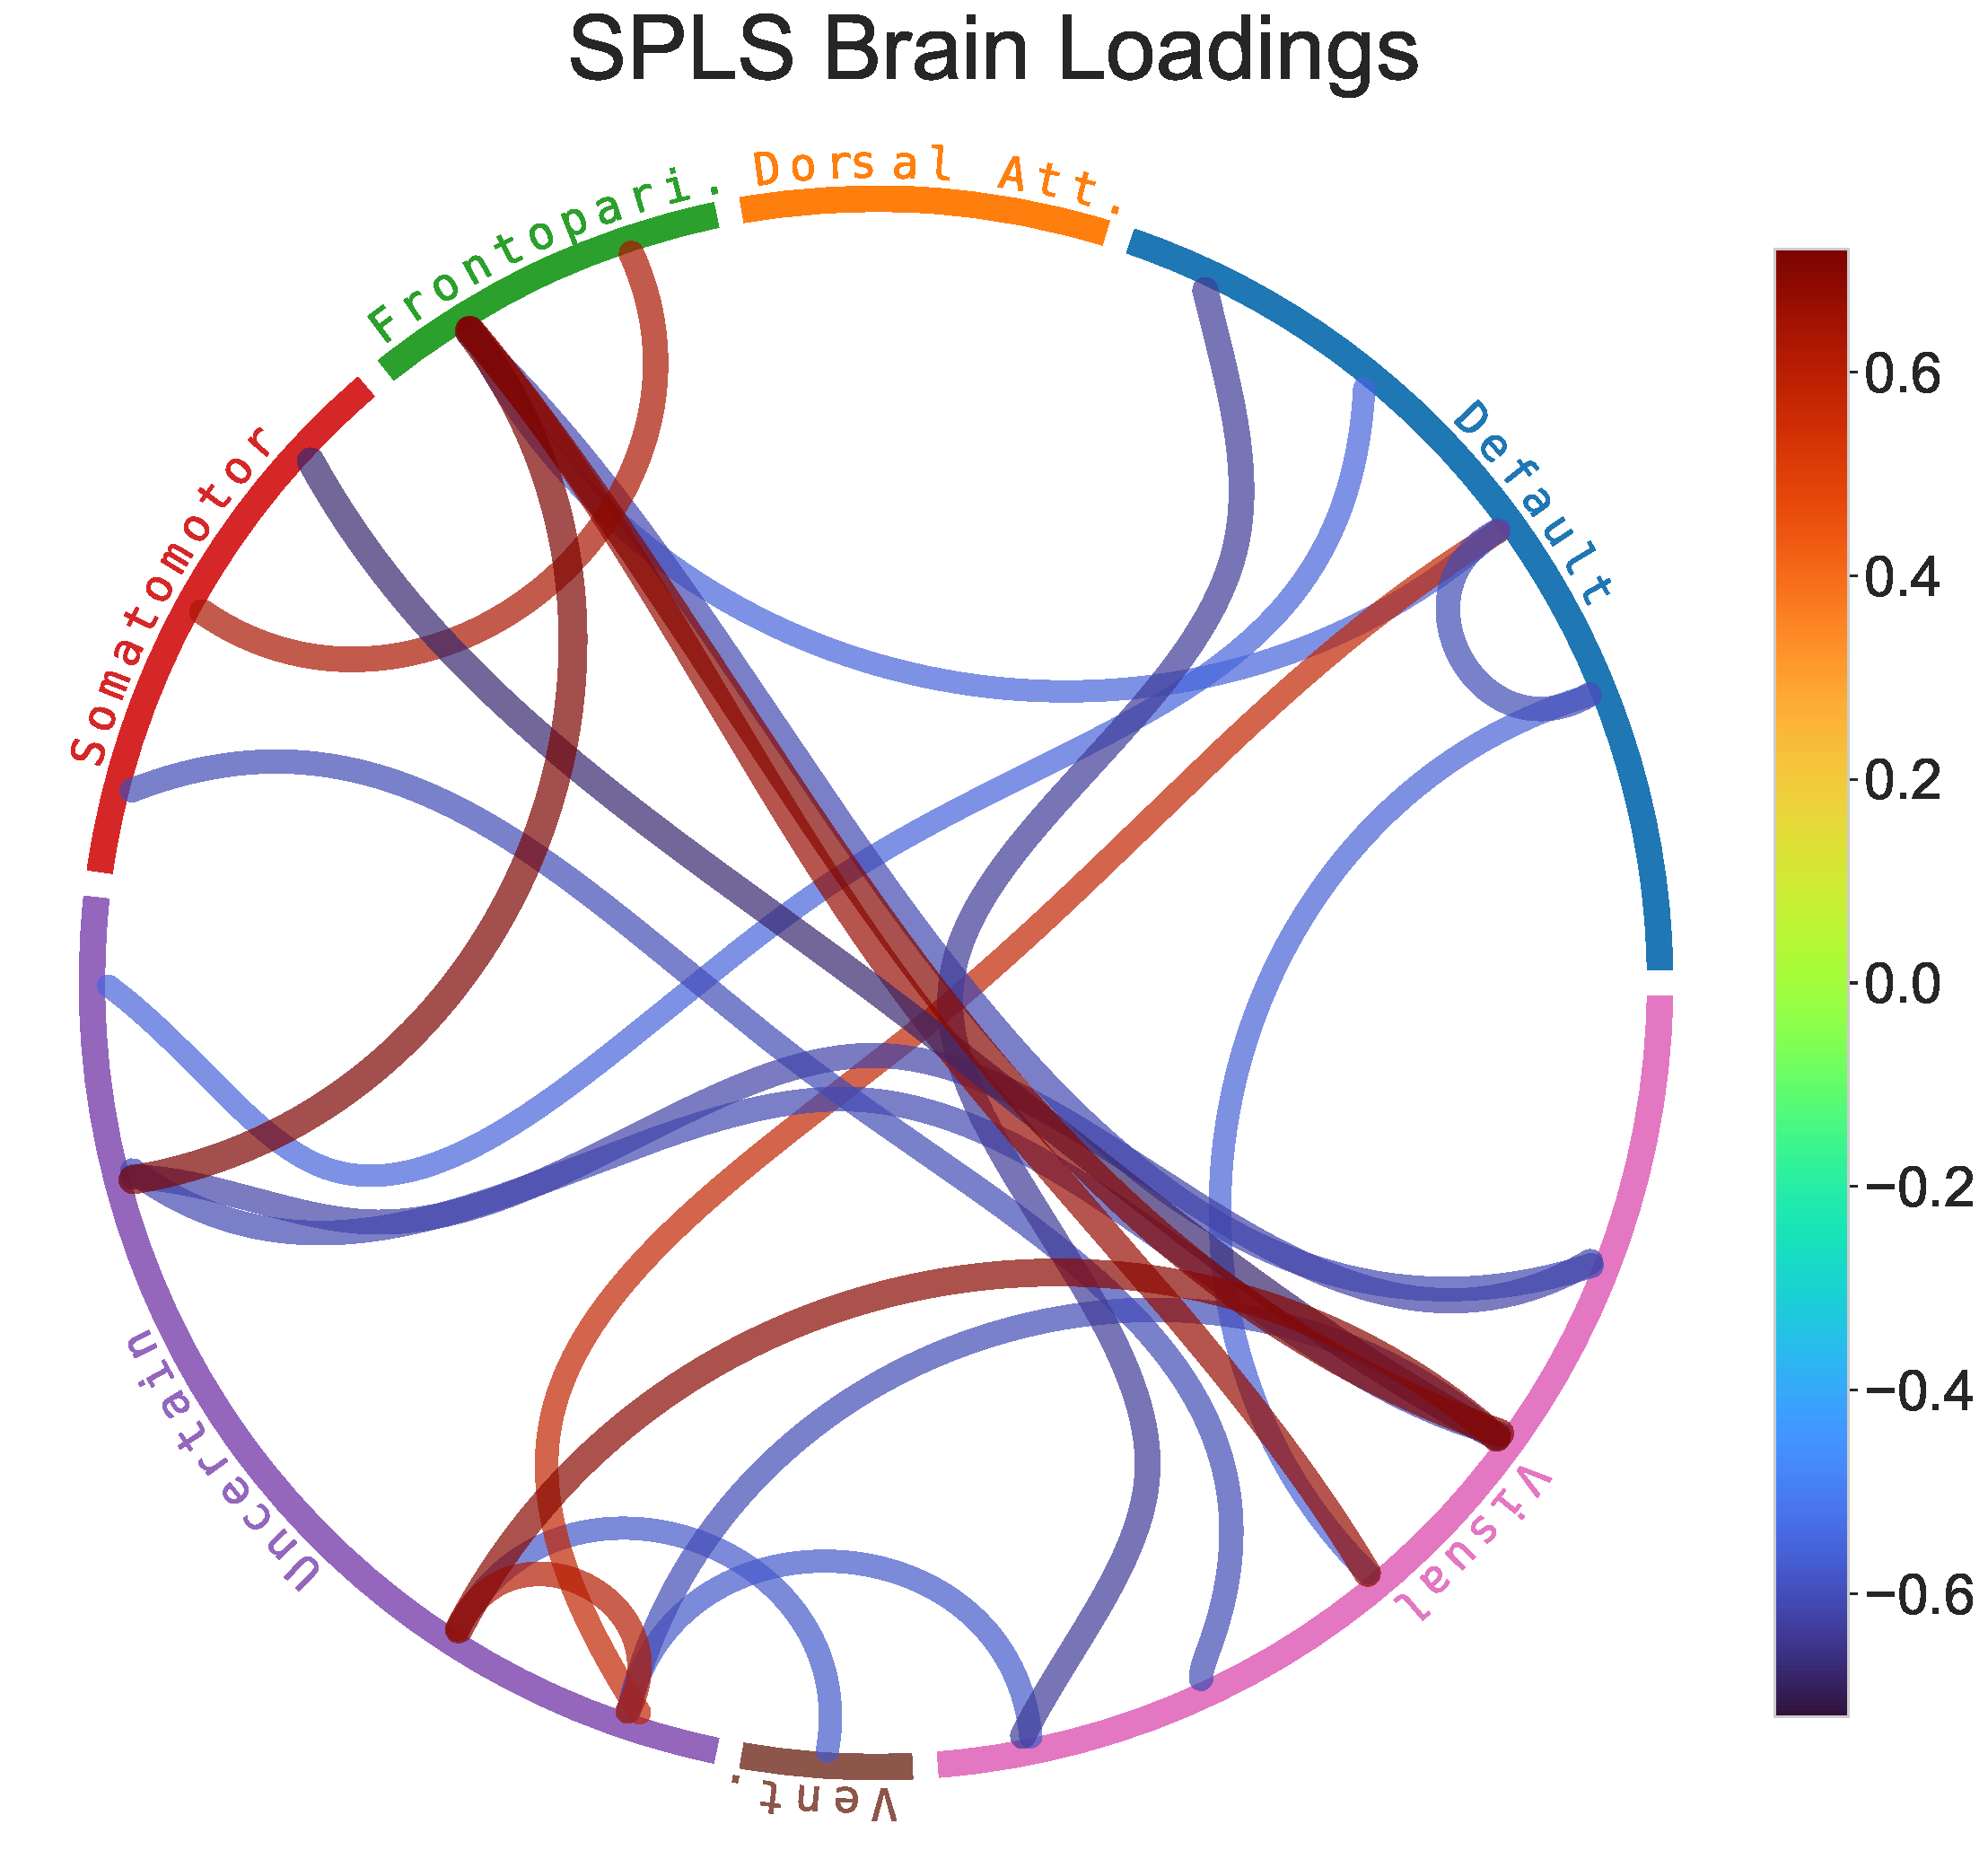
\includegraphics[width=0.49\linewidth]{figures/regularization/hcp/SPLS brain loadings.pdf}
\caption{}\label{}
\end{figure}

\subsubsection{Surface Map Parcellations}
To visualize the brain loadings, we employ a similar approach to \citep{ferreira2022hierarchical, smith2015positive}.
The brain surface plots in Figure~\ref{fig:brain} thus represent maps of brain connection strength increases/decreases, which
were obtained by weighting each node’s parcel map with the GFA edge-strengths summed across the edges
connected to the node.

\begin{figure}
\centering
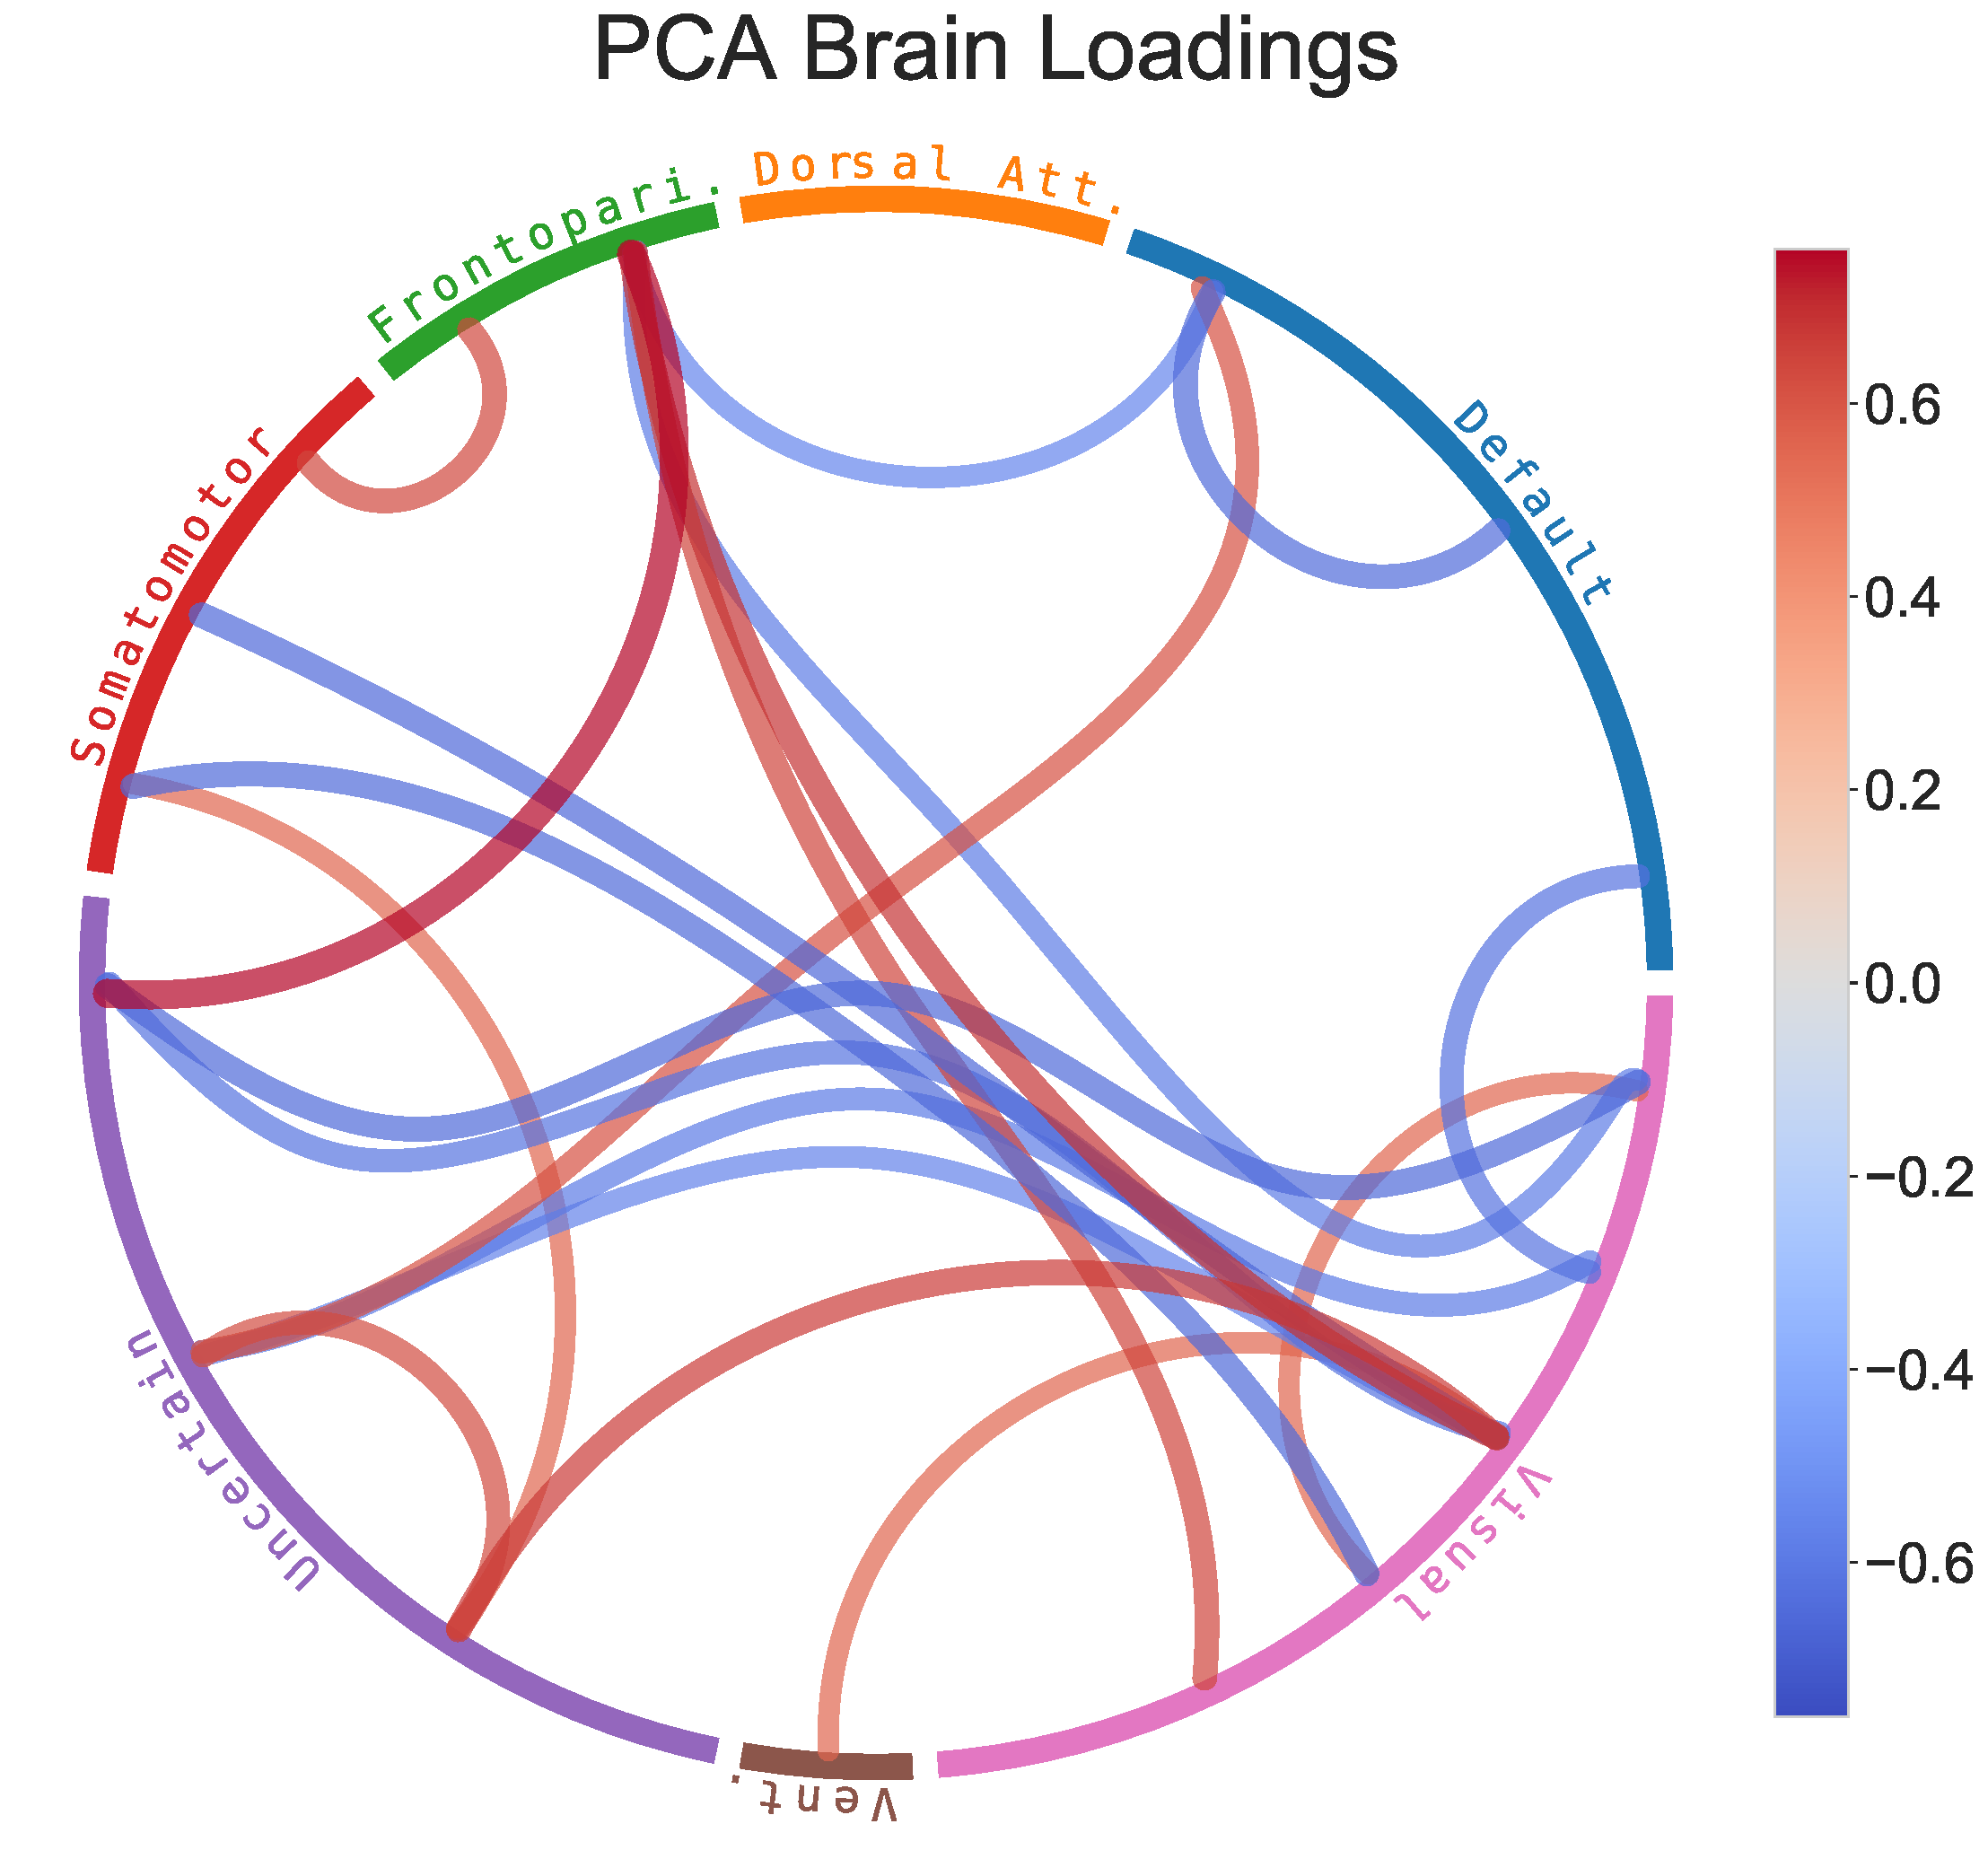
\includegraphics[width=0.68\linewidth]{figures/regularization/hcp/PCA brain loadings.pdf}
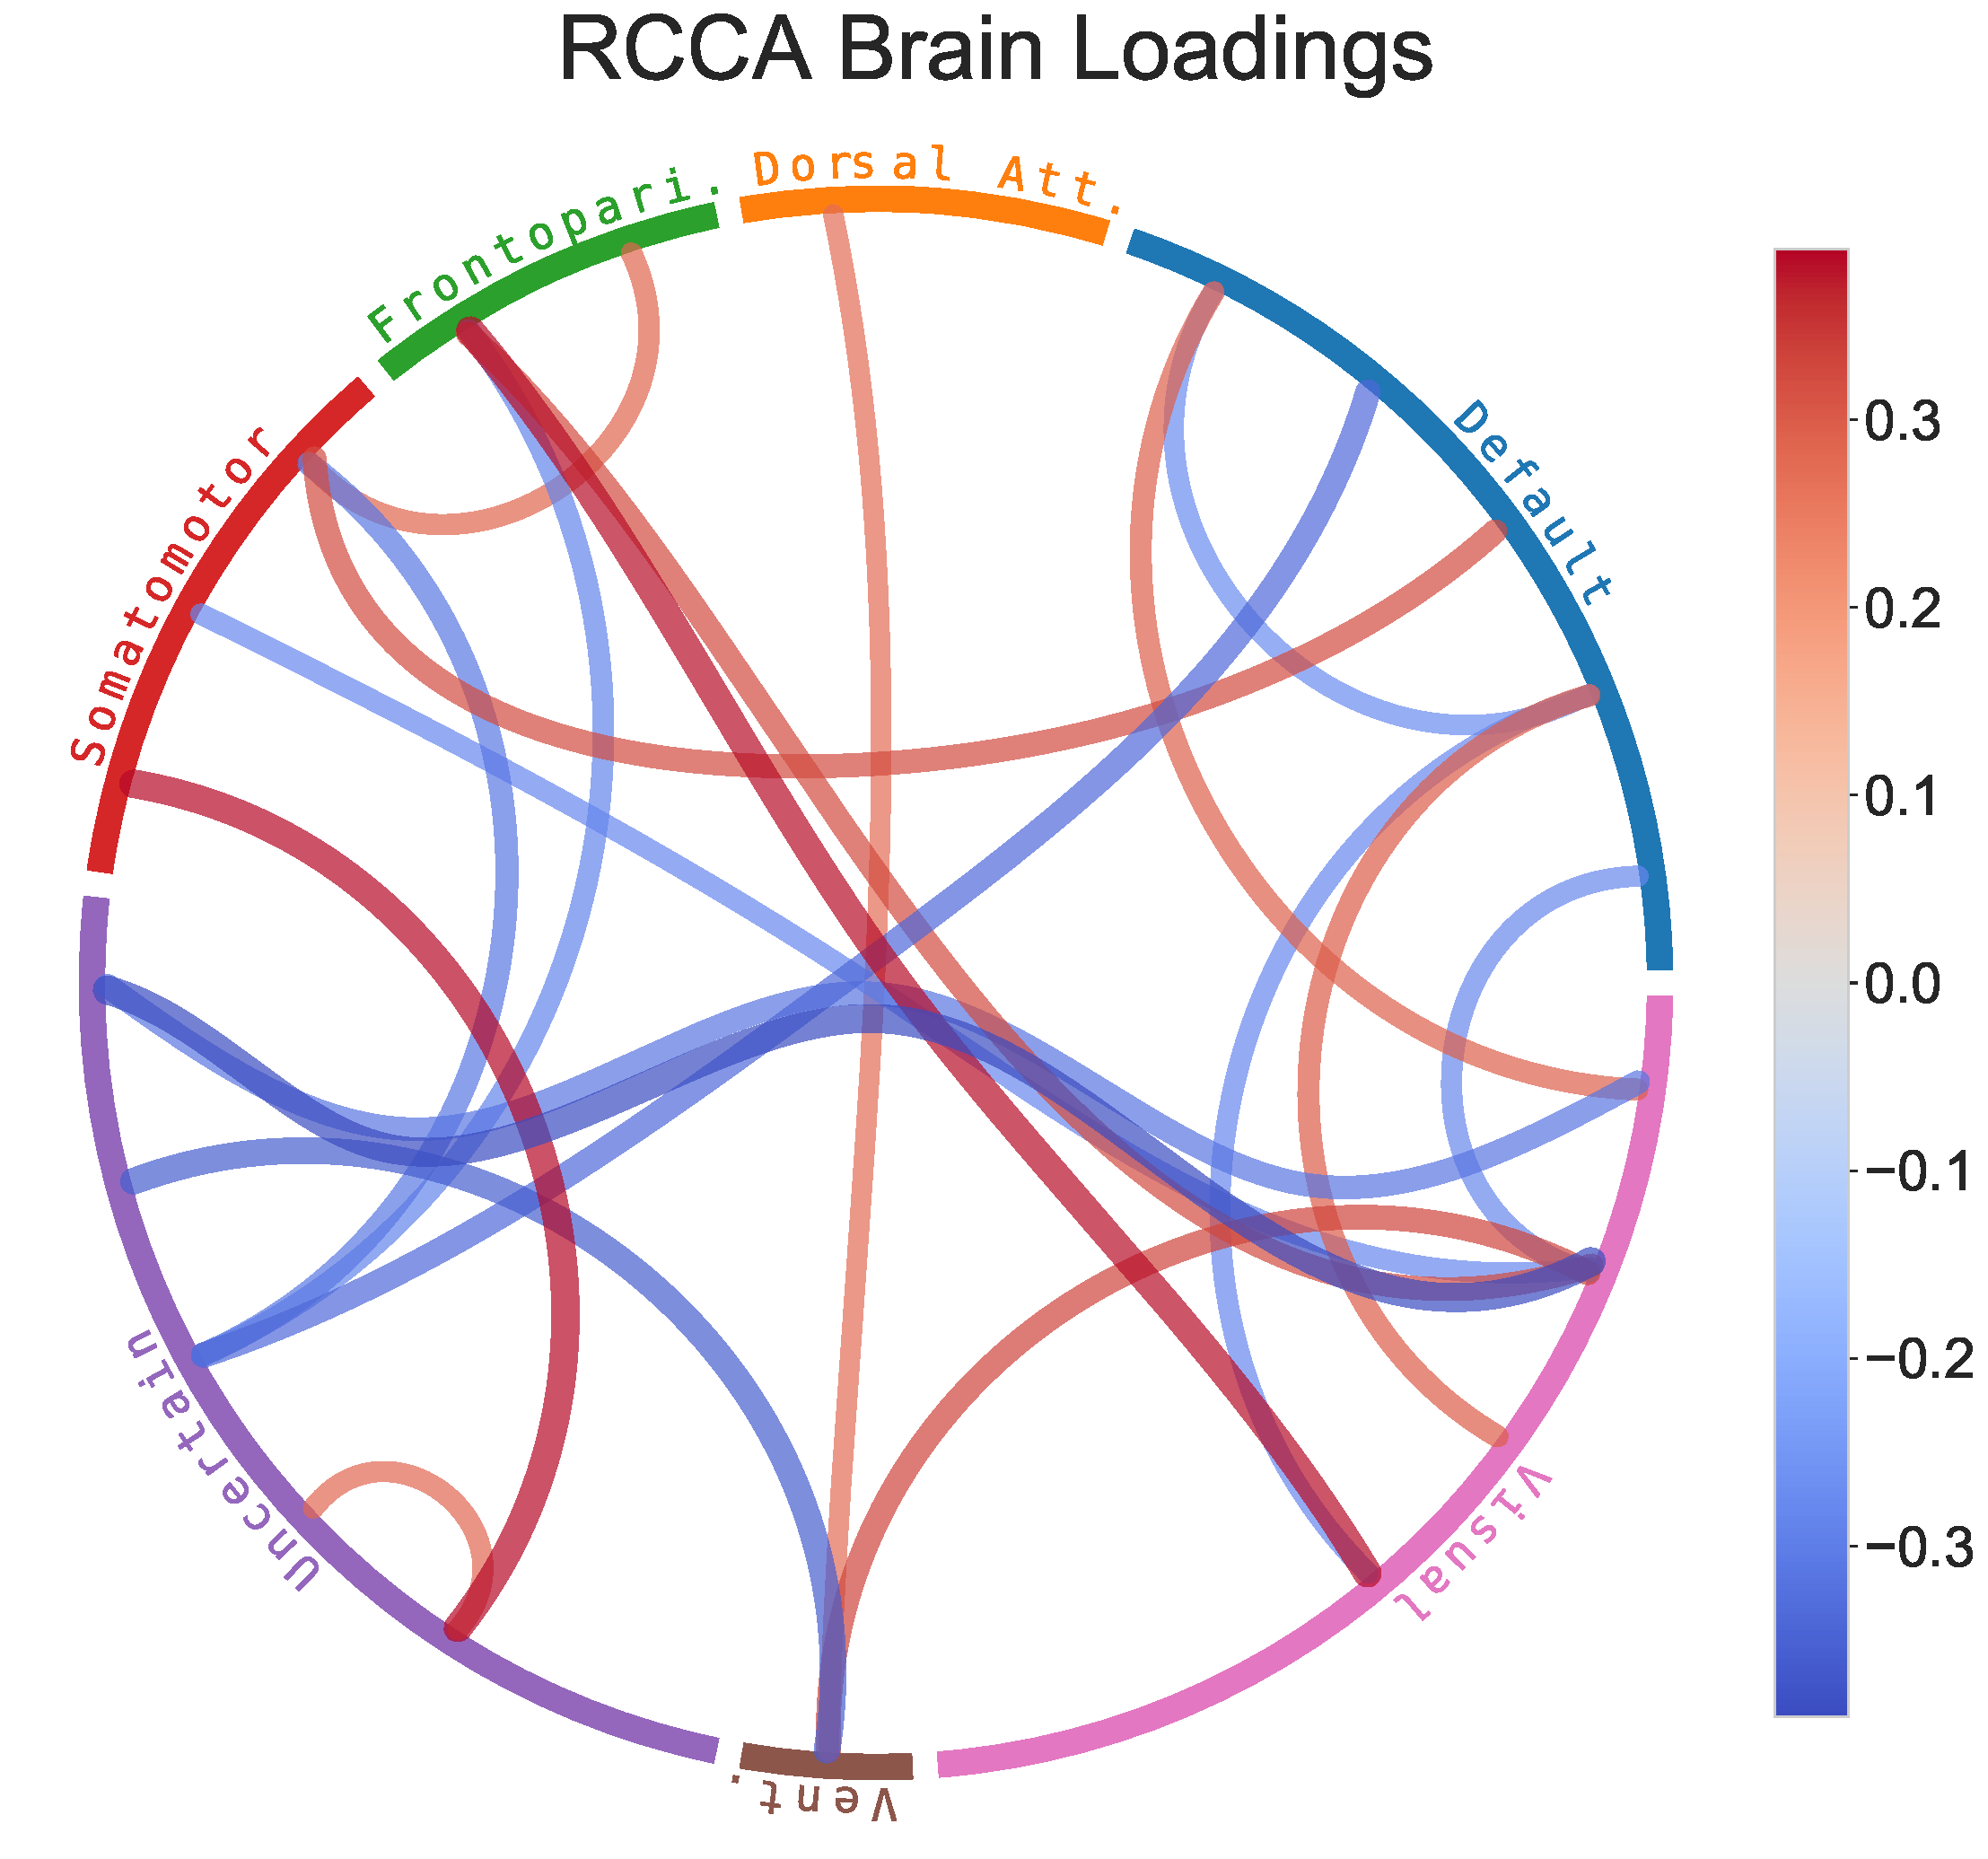
\includegraphics[width=0.68\linewidth]{figures/regularization/hcp/RCCA brain loadings.pdf}
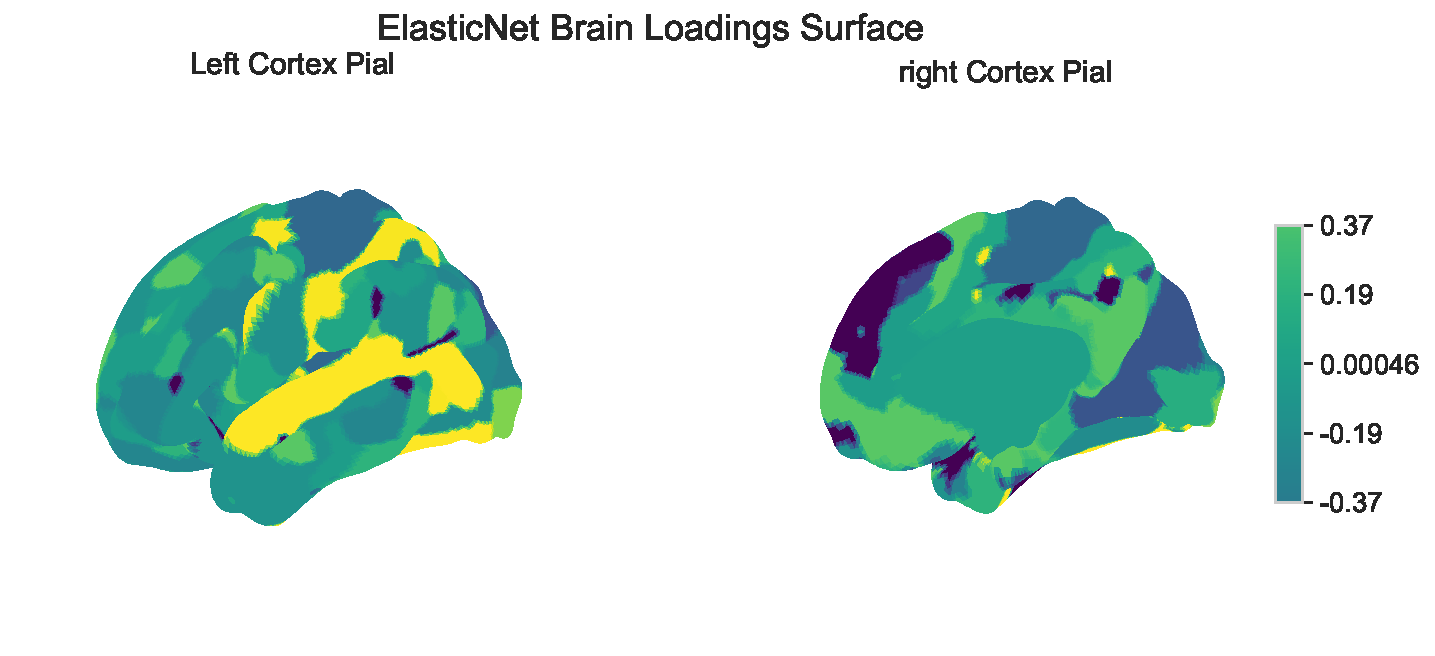
\includegraphics[width=0.68\linewidth]{figures/regularization/hcp/ElasticNet brain loadings.pdf}
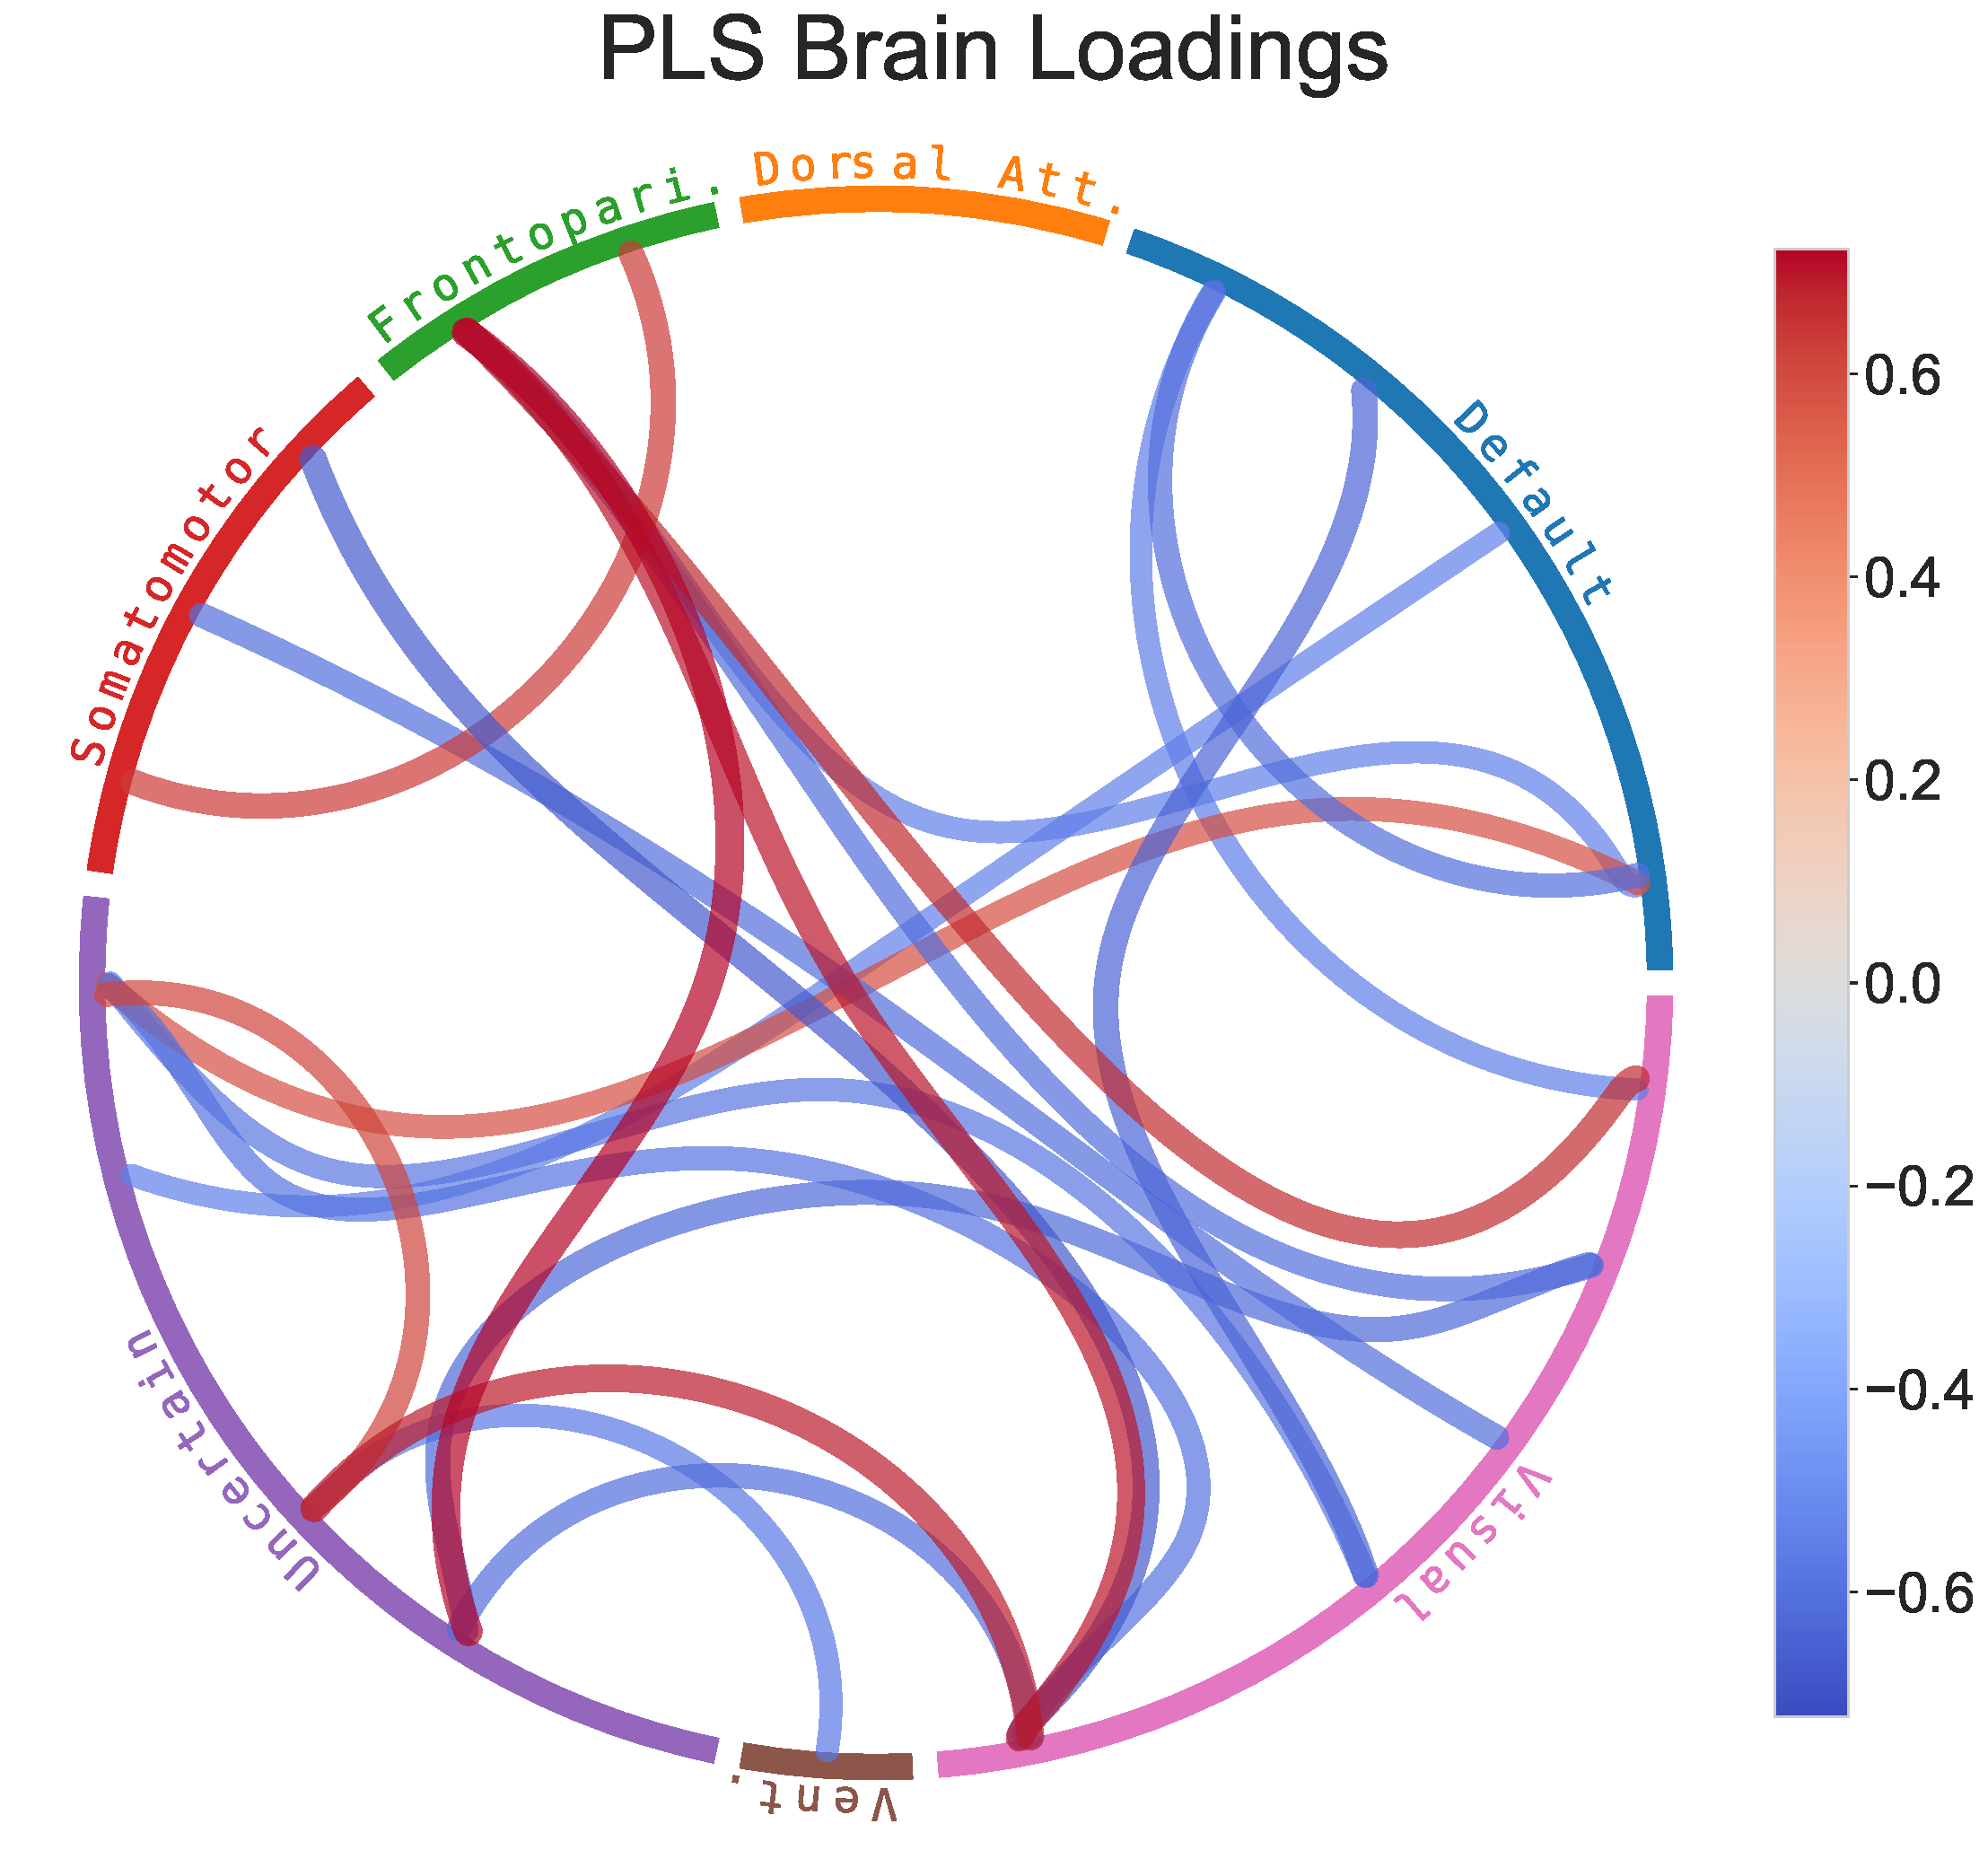
\includegraphics[width=0.68\linewidth]{figures/regularization/hcp/PLS brain loadings.pdf}
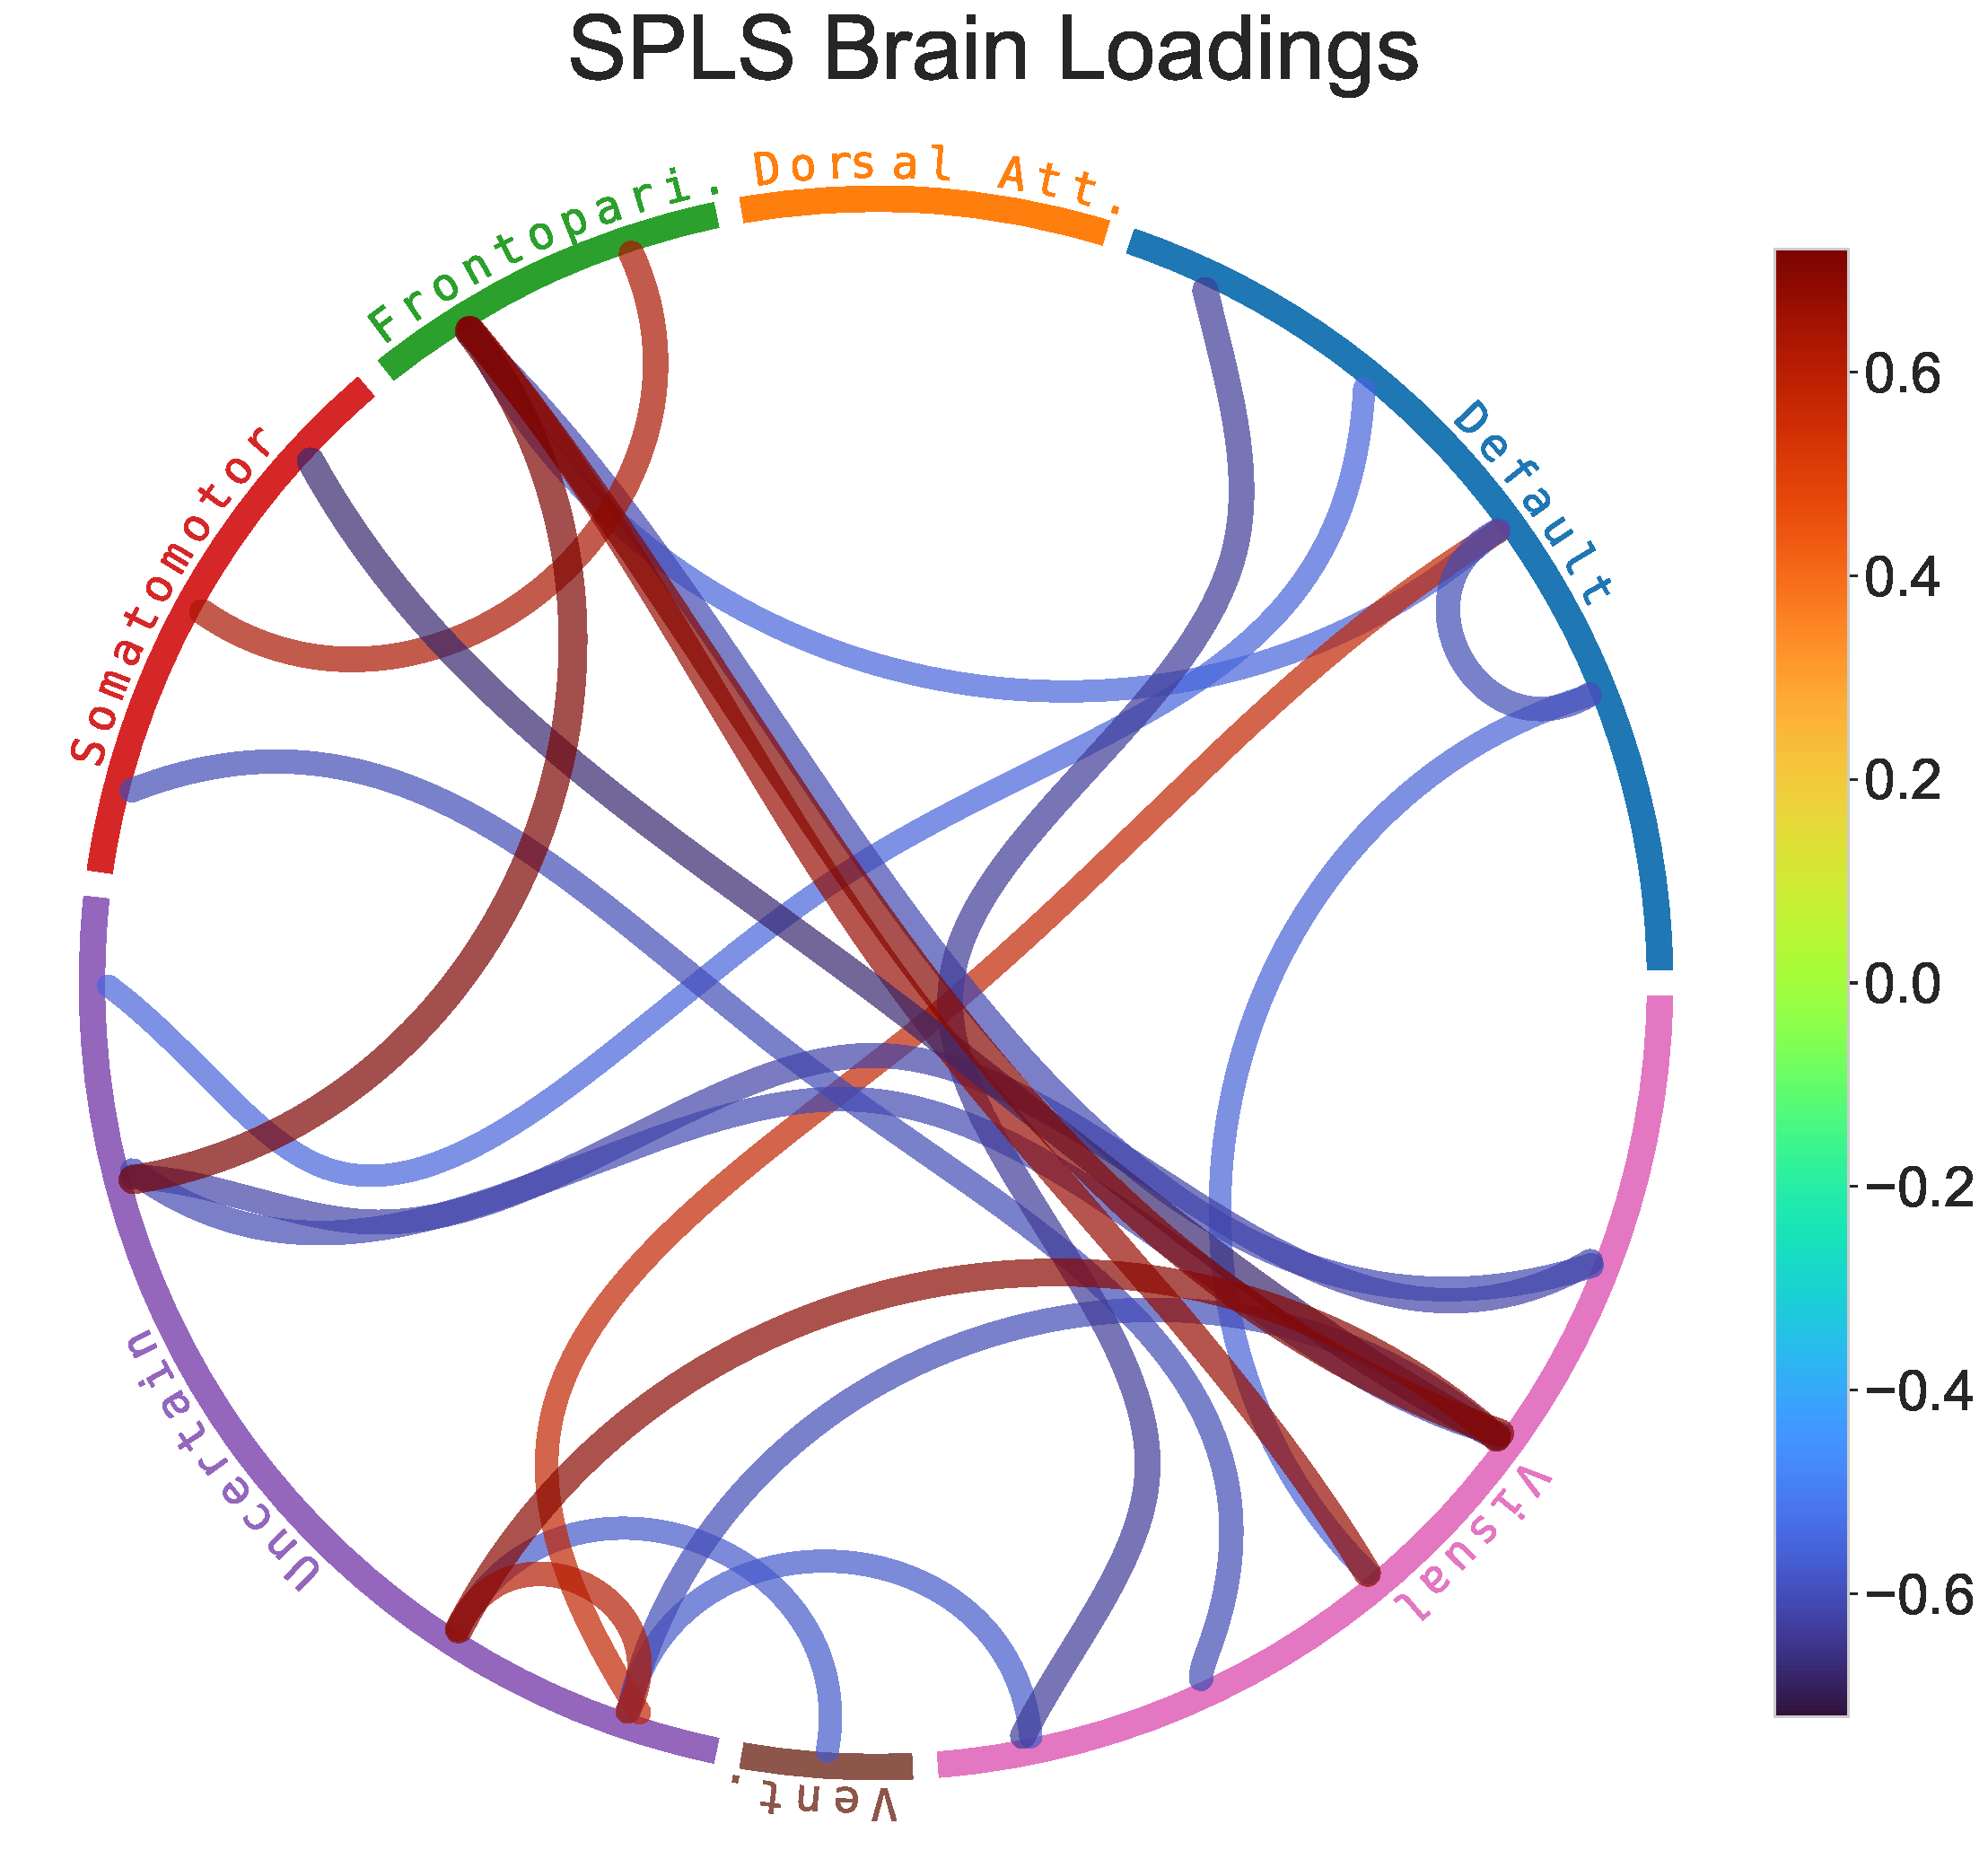
\includegraphics[width=0.68\linewidth]{figures/regularization/hcp/SPLS brain loadings.pdf}
\caption{Map of CCA connection strength variations, with each node’s parcel map weighted by CCA edge-strength changes across edges involving that node.}\label{fig:brain}
\end{figure}


\paragraph{Sparsity of Weights} Something about the sparsity of weights

\begin{table}[h]
\centering
\caption{Number of non-zero weights for each model.}
\begin{tabular}{|l|c|c|}
\hline
Model &  Brain Weights &  Behaviour Weights \\
\hline
PCA        &            300 &                145 \\
RCCA       &            300 &                145 \\
ElasticNet &            241 &                 96 \\
PLS        &            300 &                145 \\
SPLS       &            118 &                 56 \\
\hline
\end{tabular}\label{table:brain-behaviour-weights}
\end{table}



\subsection{Regularized CCA with the ADNI Data}



\subsection{Measuring the Identitiness of the Covariance Matrices}

In this section, we measure the identitiness of the covariance matrices for the simulated datasets and the HCP and ADNI datasets.
The theory we developed in section~\ref{subsec:generative-perspectives-on-cca} suggests that the identitiness of the covariance matrices is crucial for understanding how imposing sparsity on the weights imposes a prior belief in sparsity on the more biologically interesting loadings.
We measure the identitiness of the covariance matrices by looking at the eigenvalues of the covariance matrices.
If the eigenvalues of the sample covariance matrix are all close to 1, then the sample covariance matrix is close to identity.
Departures from 1 indicate that the sample covariance matrix is not close to identity and imply multicollinearity in the data.

In the simulated data, we can see that the joint covariance method with identity covariance matrices, and the GFA model with an identity noise covariance matrix, have eigenvalues closer to one than the joint covariance method with random covariance matrices, and the Probabilistic CCA model with random noise covariance matrices(Figure~\ref{fig:covariance-eigenvalues-simulated}).
On the other hand, these plots (shown for 10 random samples) show that all of the sample covariance matrices depart from the ideal case, even when the true covariance matrices are identity.

\begin{figure}
\centering
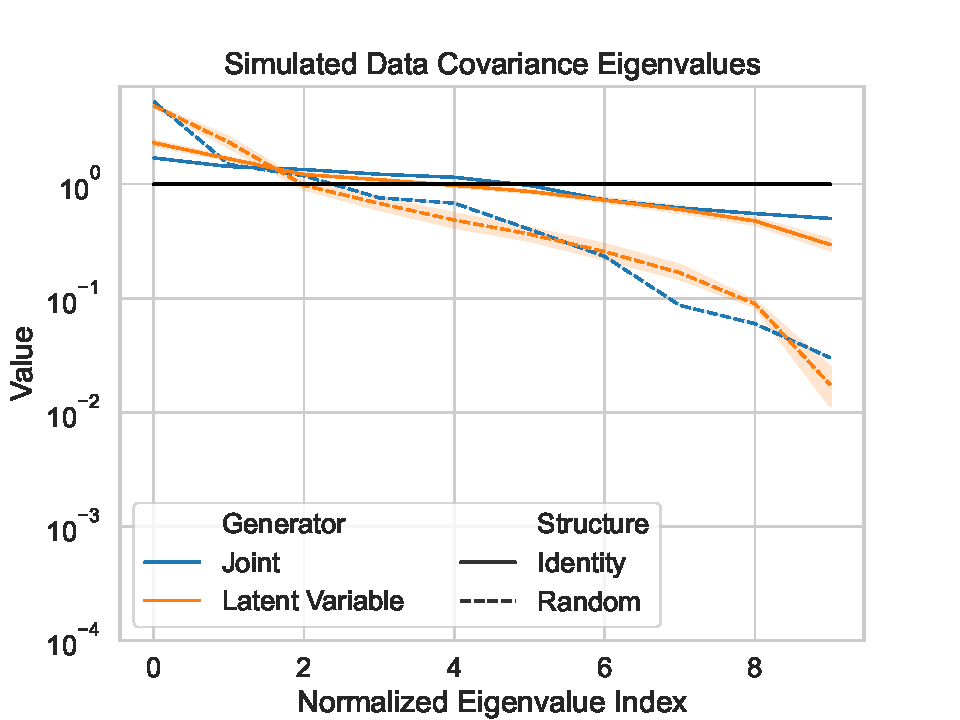
\includegraphics[width=0.8\linewidth]{figures/regularization/covariance/simulated_covariance_eigenvalues.pdf}
\caption{Eigenvalues of the covariance matrices for the simulated datasets.}\label{fig:covariance-eigenvalues-simulated}
\end{figure}

In the HCP and ADNI datasets, we can see that the only dataset and view with eigenvalues close to 1 is the ADNI brain data (Figure~\ref{fig:covariance-eigenvalues}).
This suggests that the only dataset and view where we can expect sparsity on the weights to imply sparsity on the loadings is the ADNI brain data.

\begin{figure}
\centering
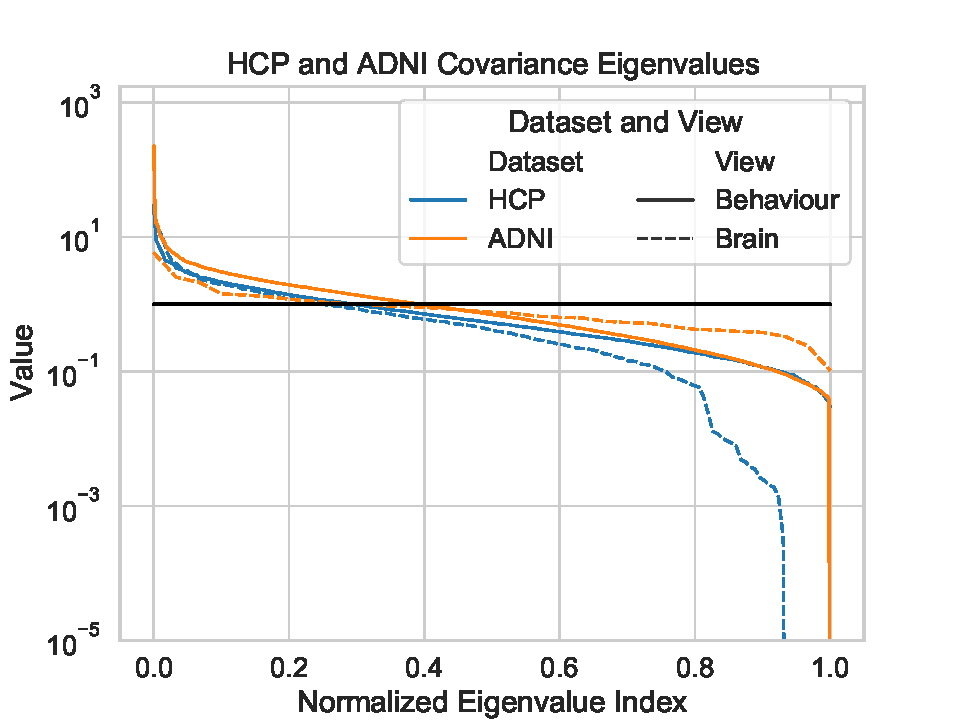
\includegraphics[width=0.8\linewidth]{figures/regularization/covariance/hcp_adni_covariance_eigenvalues}
\caption{Eigenvalues of the covariance matrices for the HCP and ADNI datasets.}\label{fig:covariance-eigenvalues}
\end{figure}

We can also see these differences by plotting the covariance matrices themselves in Figure~\ref{fig:covariance-matrices}.
In the behavioural data, which is somewhat low dimensional in both datasets, we can see the block structure of the covariance matrices.
In the brain data, we are unable to plot the whole covariance matrix because it is too high-dimensional and therefore only show a sample.


\begin{figure}
\centering
\begin{subfigure}{0.49\linewidth}
\centering
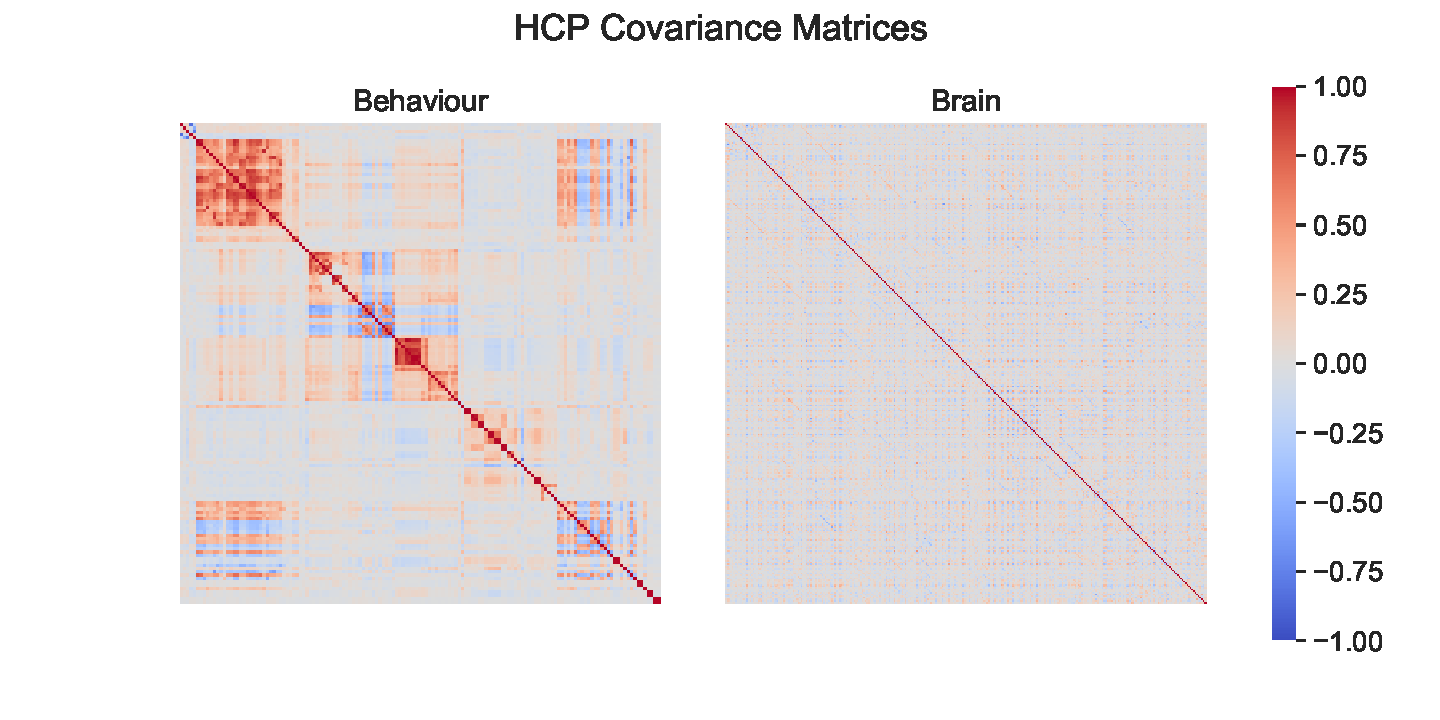
\includegraphics[width=\linewidth]{figures/regularization/covariance/HCP_covariance}
\caption{HCP}
\end{subfigure}
%
\begin{subfigure}{0.49\linewidth}
\centering
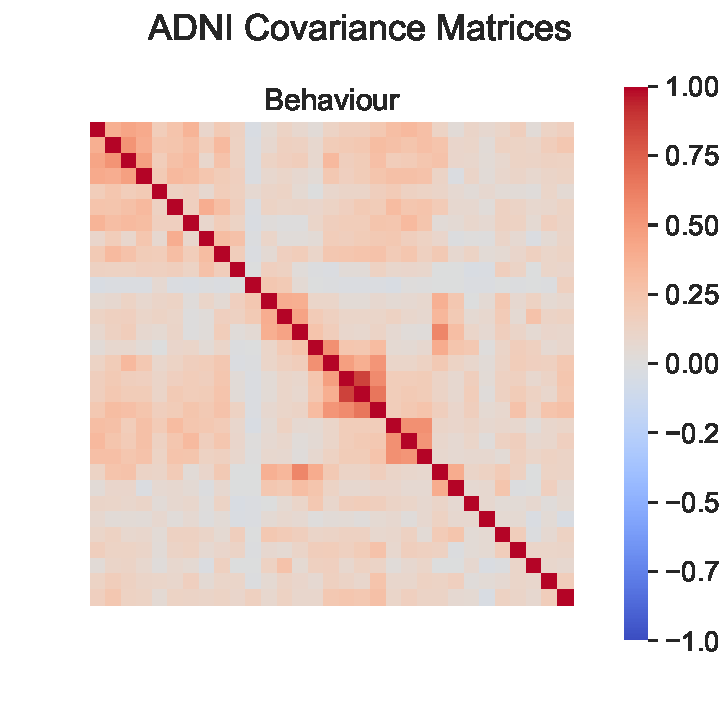
\includegraphics[width=\linewidth]{figures/regularization/covariance/ADNI_covariance}
\caption{ADNI}
\end{subfigure}
\caption{Covariance matrices for the HCP and ADNI datasets.}
\label{fig:covariance-matrices}
\end{figure}

\section{Discussion and Limitations}

In this section, we discuss the implications of our findings as well as the limitations of our approach; some of which we address in later chapters of this thesis.

\subsection{Discussion}

In this section, we outline several crucial points that emerged from our study, highlighting the considerations when using CCA and its related methods.

\subsubsection{The importance of matching the model to the data generating process}

The results showcase clear discrepancies when the underlying model does not align with the data generation process. For instance, in the \textit{Probabilistic CCA with Random Covariance Matrices} experiment, both Elastic regularization and SPLS did not enhance the performance of CCA and PLS, respectively.
This happened primarily because the real weights weren't sparse, leading to a mismatch between the model and the data generation mechanism.
These findings underscore the necessity of selecting models that mirror the intrinsic structure and nature of the data.
Inaccurate model selection can result in suboptimal outcomes, even with sophisticated regularization techniques in place.

\subsubsection{Sample versus population settings can lead to different outcomes}

The results from the \textit{Joint Covariance and Sparse Weights} experiment exemplify the disparities that can arise between population and sample settings.
Although PLS, RCCA, and CCA are equivalent under isotropic noise in a population framework, their performance can vary substantially in a sample setting.
This phenomenon exemplifies the inherent challenges that can arise when interpreting outcomes in sample settings.
It's therefore crucial for researchers to recognize these nuances and adopt appropriate measures when extrapolating results, particularly because in brain-behaviour studies, we only have one sample and its size is often limited.

\subsubsection{FRALS allows for flexible regularization for closer model matching}

Our results show that when true weights are sparse and maximal ridge regularization is not needed (i.e. SPLS), FRALS with elastic net regularization can be much more effective at recovering the true weights in simulated data.

\subsubsection{Sparsity on the weights does not imply sparsity on the loadings}

On the other hand, our results raise the question of whether sparsity on the weights makes sense in the first place.
For latent variable models of brain-behaviour associations, we have argued that the loadings are the more biologically relevant quantity.
Since in practice identity covariance is rarely a good assumption, the weights and loadings are not equivalent.
This means that sparsity on the weights does not imply sparsity on the loadings and so we should not expect sparsity on the weights to lead to more interpretable loadings.
A practical step this implies is \textit{to ensure that the data covariances are at least close to identity before applying sparse CCA methods}.

\subsubsection{ElasticNet finds a subtly different mode to other models in the HCP data}

RCCA and ElasticNet gave more weight to the parietal lobe than PCA and PMD did.
This suggests that our model finds the parietal lobe more relevant for capturing brain-behaviour correlations.
PMD focused on principal components in the brain.
This could mean PMD might miss the true associations between views.
In this setting, ElasticNet functions similarly to a sparse RCCA.

\subsection{Limitations}
While FRALS offers promising performance in terms of out-of-sample correlation, it does come with significant drawbacks, the most noteworthy being its computational inefficiency.
Below, we outline the primary factors contributing to the slow speed of FRALS and provide some insights into the computational bottlenecks.

\subsubsection{Computational Time}\label{subsec:computational-time}
While computationally intensive, the flexibility of FRALS allows it to adapt better to the complexity inherent in real-world data sets, such as the HCP. This adaptability could be crucial when high predictive accuracy or interpretability is required.

\subsubsection{Changing Regression Targets}\label{subsec:changing-regression-targets}
Adding to the computational burden is the fact that the regression targets, i.e., the projections of the other view, are not static but change dynamically throughout the algorithm's run.
Each update to the least squares solution consequently alters the global objective, leading to a constantly shifting landscape that the algorithm needs to navigate.

\section{Conclusions}

We delved into the relationship between CCA's backward and forward models.
Our findings suggest that the backward model's weights don't guarantee sparsity in the forward model's loadings.
Therefore, looking at the loadings might offer more meaningful biological insights.

We also introduced and incorporated elastic net regularization using alternating least squares to improve CCA model regularization.

We used simulated data to shine light on the challenges of interpreting the results of CCA studies, even when we know the true data generation process.
We showed the effect of different regularization techniques, the population and sample settings, loadings and weights.
We also showed clearly that PLS behaves as a heavily regularised version of CCA and is often inappropriate.
SPLS is similarly flawed despite its popularity.

In the real Brain-Behaviour data from the Human Connectome Project, we found that ...

In summary, our study underscores the need to choose the right model for specific data situations.